\documentclass[twoside,12pt]{report}
% ============================================================ EX-TEST
\usepackage[utf8]{vietnam}
%\usepackage{ex_test}
\usepackage[solcolor]{ex_test} % dethi, color, loigiai, solcolor, book
\renewtheorem{ex}{\color{blue!90!black} Câu}
\usepackage{amsmath,amssymb,tikz,mathrsfs,tkz-tab}
\usepackage{fontawesome}
\usepackage[many]{tcolorbox}
\usetikzlibrary{calc}
\usepackage{geometry}
\renewcommand{\baselinestretch}{1.5}
\usepackage[locale=DE]{siunitx} % cách viết số đo có đơn vị theo chuẩn DE (gần giống VN) 
\usepackage{setspace} % hỗ trợ định dạng khoảng cách văn bản.
\usepackage[newparttoc]{titlesec}	% định dạng tiêu đề cho các section
\usepackage{currfile}
\usepackage[version=3]{mhchem} % công thức và phương trình hóa học 
\usepackage{tikz} % gói TikZ vẽ hình 
	\usetikzlibrary{decorations.shapes,shapes.geometric,calc,positioning}
\usepackage{pgf} % hỗ trợ phép tính toán học và vẽ hình	
\usetikzlibrary{shapes.geometric, arrows}
\usepackage{pgfplots}
\renewcommand{\baselinestretch}{1.2}
\usepackage{tabularx}
\usepackage{makecell}
\usepackage{titlesec}
\usepackage{titletoc}
\usepackage{colortbl}
\usepackage{tkz-euclide}
% lệnh siunit 
\newcommand{\xsi}[2]{\SI[parse-numbers=false]{#1}{#2}}
\newcommand{\outfooter}{
\color{purple}\bfseries	GV: Lương Hoàng Sang
}
\newcommand{\outheader}{
	\color{purple}\bfseries	Trường THCS - THPT Nguyễn Khuyến
}
\newcommand{\namhoc}{
	\color{purple}\bfseries	Năm học: 2024 - 2025
}
\def\monhoc{\bfseries Vật lí 10}%{\bfseries Kế hoạch bài dạy vật lí 10}
\graphicspath{{figs/}{extra/}} % các thư mục chứa hình ảnh 

% ========== PAPER FORMAT ====================
% --- paper size 
\geometry{
	a4paper	% khổ giấy A4
	,total={180mm,260mm} % kích thước văn bản A4 170mmx247mm
	,left=15mm % canh lề trái
	,top=20mm % canh lề trên
	,footskip=1.0cm % khoảng cách từ văn bản đến footer
}
% --- line spacing -- choose 1 in 2 choices 
\onehalfspacing			% cách dòng đơn
%\doublespacing			% cách dòng đôi  
	% ----- định dạng Header và footer
		% --- 
	\newlength\sectitleindent
	\setlength\sectitleindent{0.5cm}
	\newlength\subsectitleindent
	\setlength\subsectitleindent{1cm}
% --- trang văn bản thông thường  
\pagestyle{fancy} 
\fancyhf{}
\renewcommand{\headrulewidth}
{1pt} % độ dày đường kẻ ở header 
\newcommand*\cirpage[1] % tạo hình tròn quanh số trang 
{\tikz[baseline=(char.base)]
	{
		\node[
		shape=circle
		,draw=black
		,fill=gray!0
		,inner sep=2pt
		]
		(char)
		{#1};
	}
}
\fancyhead[LO,RE] % footer - lề trong 
{	
\small \outheader \hfill \namhoc% tên tài liệu lấy từ phần khai báo đầu file 
}  
\fancyfoot[LO,RE] % footer - lề trong 
{	
	\small \outfooter % tên tài liệu lấy từ phần khai báo đầu file 
}  
\fancyfoot[CO,CE] % footer - giữa trang 
{
	\small \cirpage{\thepage}
} 
\fancyfoot[LE] % footer - lề ngoài 
{
	\hspace{-\sectitleindent}
	\vspace*{-11pt}
	{\color{purple} \monhoc}
}
\fancyfoot[RO] % footer - lề ngoài 
{
	\hspace{-\sectitleindent}
	\vspace*{-11pt}
	{\color{purple} \monhoc}\hspace*{-5pt}
}
% --- trang Part và Chapter title 
\fancypagestyle{plain} % mặc định của trang Part và Chapter title 
{
	\fancyfoot[LO,RE]
	{
		\hspace{-\sectitleindent}\small \outfooter
	}
	\fancyfoot[CO,CE]
	{
		\small \cirpage{\thepage}
	} % footer - giữa trang chẵn và lẻ 
	\fancyfoot[LE]
	{
		\hspace{-\sectitleindent}
		\vspace*{-11pt}
		\hspace*{-1.1pt}{\color{purple}\monhoc}
	}
	\fancyfoot[RO]
	{
		\hspace{-\sectitleindent}
		\vspace*{-11pt}
		{\color{purple}\monhoc}\hspace*{-5pt}
	}
} % giống với trang thường 
% ký hiệu từ font Boondox 
\DeclareFontFamily{U}{BOONDOX-cal}{\skewchar\font=45 }
\DeclareFontShape{U}{BOONDOX-cal}{m}{n}{
	<-> s*[1.05] BOONDOX-r-cal}{}
\DeclareFontShape{U}{BOONDOX-cal}{b}{n}{
	<-> s*[1.05] BOONDOX-b-cal}{}
\DeclareMathAlphabet{\bdx}{U}{BOONDOX-cal}{m}{n}
\SetMathAlphabet{\bdx}{bold}{U}{BOONDOX-cal}{b}{n}
\DeclareMathAlphabet{\bbdx}{U}{BOONDOX-cal}{b}{n}
\newcommand{\calE}{\bdx{E}}
\newcommand{\calP}{\bdx{P}}
\newcolumntype{C}[1]{>{\centering\arraybackslash}p{#1}}
\newcolumntype{M}[1]{>{\centering\arraybackslash}m{#1}}
\newcolumntype{L}[1]{>{\raggedright\arraybackslash}p{#1}}
\newcommand{\hoac}[1]{ %hệ hoặc
	\left[\begin{aligned}#1\end{aligned}\right.}
\newcommand{\heva}[1]{ %hệ và
	\left\{\begin{aligned}#1\end{aligned}\right.}
% Định nghĩa lại \part
%\renewcommand{\thepart}{\arabic{part}}
%\titleformat{\part}{\normalfont\bfseries}{Chương ~ \thepart.}{0.4em}{}
% Định nghĩa lại \chapter
\titleformat{\chapter}{\centering\LARGE\bfseries}{}{0pt}{}
\titlespacing{\chapter}{0pt}{-25pt}{6pt}
% section đánh số La Mã
\renewcommand{\thesection}{\Roman{section}}
\titleformat{\section}
{\normalfont\bfseries}{\thesection.}{0.4em}{}
% Định nghĩa subsection theo A, B, ...
\renewcommand{\thesubsection}{\Alph{subsection}}
\titleformat{\subsection}[block]
{\normalfont\bfseries\hspace{1.5em}}{\thesubsection.}{0.4em}{}
% Định dạng lại kiểu đánh số equation
\renewcommand{\theequation}{\arabic{equation}}   
% Định dạng lại bảng
\renewcommand{\theadfont}
{
	\normalfont\bfseries
} % làm ô trong bảng canh giữa + in đậm 
\setcounter{secnumdepth}{4} % đánh số đến cấp thứ 4 của chỉ mục (subsubsection sẽ được đánh số)
\renewcommand{\thesubsubsection}{\arabic{subsubsection}}
\titleformat{\subsubsection}
{\normalfont\bfseries}{Hoạt động~\thesubsubsection:}{0.4em}{}
%%%%%%%%%%%%%%%% Định nghĩa môi trường Hoạt động
\newcommand{\hoatdong}[4]
{
	\subsubsection{#1}
	\begin{enumerate}[label=\bfseries\itshape \arabic*., topsep=0pt, itemsep=0ex]
		\item \textbf{\textit{Mục tiêu}}\\
		#2
		\item \textbf{\textit{Sản phẩm học tập}}\\
		#3
		\item \textbf{\textit{Tổ chức hoạt động}}\\
		#4
	\end{enumerate}
	
}
%======== MAIN TABLE OF CONTENTS
\contentsmargin{1.5em}	
\titlecontents{part}
[3cm] % Left indentation
{
} % Spacing and font options for parts
{}
{}
{}
[\addvspace{5pt}\color{black}]

% Chapter text styling
\titlecontents{chapter}
[1.25cm] % Left indentation
{} % Spacing and font options for chapters
{} % Formatting of numbered sections of this type
{} % Formatting of numberless sections of this type
{} % Formatting of the filler to the right of the heading and the page number
\begin{document}
		% ---------	Table of Contents (ToC) ---------
%	\tableofcontents
	
% ====================================================== input data Bài 1
%\part{CHƯƠNG 1}
%\chapter{Bài 7. Gia tốc - Chuyển động thẳng biến đổi đều }
\begin{center}
	\bfseries\itshape (4 tiết)
\end{center}
\section{MỤC TIÊU DẠY HỌC}
\begin{center}
	\begin{longtable}{|M{2.5cm}|L{12.5cm}|M{2cm}|}
		\hline
		\thead{Biểu hiện\\ năng lực} & \thead{Mục tiêu} & \thead{STT}\\
		\hline
		\multicolumn{3}{|c|}{\textbf{ Năng lực vật lí}}\\
		\hline
		1.1 & Lập luận dựa vào sự biến đổi vận tốc trong chuyển động thẳng, rút ra được công thức tính gia tốc.  & 1\\
		\hline
		1.1 & Nêu được ý nghĩa, đơn vị của gia tốc.  & 2\\
		\hline
		1.2 & Dựa trên số liệu cho trước vẽ được đồ thị vận tốc – thời gian trong chuyển động thẳng. & 3\\
		\hline
		1.2 & Vận dụng đồ thị vận tốc – thời gian để tính được độ dịch chuyển và gia tốc trong một số trường hợp đơn giản. & 4\\
		\hline
		1.2 & Rút ra được các công thức của chuyển động thẳng biến đổi đều (không được dùng tích phân). & 5\\
		\hline
		1.2 & Vận dụng được các công thức của chuyển động thẳng biến đổi đều. & 6\\
		\hline
		\multicolumn{3}{|c|}{\textbf{Năng lực chung}}\\
		\hline
		GT - HT & Chủ động trong giao tiếp khi làm việc nhóm; biết khiêm tốn tiếp thu sự góp ý và nhiệt tình chia sẻ, hỗ trợ các thành viên trong nhóm. & 7\\
		\hline
		TC - TH & Chủ động, tích cực thực hiện các nhiệm vụ được đặt ra cho các nhóm; tự điều chỉnh thái độ, hành vi của bản thân, bình tĩnh và có cách cư xử đúng khi giao tiếp trong quá trình làm việc nhóm. & 8\\
		\hline
	\end{longtable}
\end{center}
\section{THIẾT BỊ DẠY HỌC VÀ HỌC LIỆU}
\begin{itemize}
	\item Tivi/máy chiếu.
	\item Phiếu thảo luận nhóm.
\end{itemize}
\section{TIẾN TRÌNH DẠY HỌC}
\subsection{TIẾN TRÌNH}
\begin{center}
	\begin{longtable}{|L{2.75cm}|C{1.25cm}|L{5cm}|L{3.5cm}|L{4cm}|}
		\hline
		\thead{Tiến trình} & \thead{Mục\\tiêu} & \thead{Nội dung dạy học \\trọng tâm} & \thead{PP,\\ KTDH} & \thead{Phương pháp \\đánh giá}\\
		\hline
		\textbf{Hoạt động 1:} Tìm hiểu khái niệm và ý nghĩa của gia tốc. & 1, 2, 7, 8 & Công thức tính gia tốc, ý nghĩa và đơn vị của gia tốc.&PP: Dạy học giải quyết vấn đề, thuyết trình. & GV đánh giá dựa trên kết quả báo cáo thảo luận nhóm của HS.\newline
		PP đánh giá: quan sát, nghe.\\
	\hline
	\textbf{Hoạt động 2:} Vận dụng đồ thị vận tốc – thời gian để tính độ dịch chuyển và gia tốc. & 3, 4, 7, 8 & Đồ thị vận tốc – thời gian trong chuyển động thẳng biến đổi đều.\newline
	Vận dụng đồ thị vận tốc – thời gian để tính độ dịch chuyển và gia tốc trong trường hợp đơn giản.
	& PP dạy học: Dạy học hợp tác, thuyết trình.\newline
	KTDH: Chia sẻ cặp đôi.
	& GV đánh giá dựa trên kết quả trên phiếu học tập và bài báo cáo của nhóm HS.\newline
	PP đánh giá: quan sát, nghe.\\
	\hline
	\textbf{Hoạt động 3:} Rút ra các công thức của chuyển động thẳng biến đổi đều. & 5, 7, 8 & Các công thức chuyển động thẳng biến đổi đều. & PP: Dạy học hợp tác. & GV đánh giá dựa trên kết quả hoạt động nhóm của HS trên phiếu học tập.\newline
	PP đánh giá: quan sát, nghe.\\
	\hline
	\textbf{Hoạt động 4:} Luyện tập. & 3, 4, 6 & Vận dụng các công thức chuyển động thẳng biến đổi đều. & PP: Đàm thoại & GV đánh giá dựa trên bài tập cá nhân của HS.\newline
	PP đánh giá: quan sát.\\
	\hline
	\end{longtable}
\end{center}
\subsection{CÁC HOẠT ĐỘNG HỌC}
\subsubsection{Hoạt động 1. Tìm hiểu khái niệm và ý nghĩa của gia tốc}
\begin{enumerate}[label=\bfseries\itshape \arabic*.]
	\item \textit{\textbf{Mục tiêu}}\\
	\begin{itemize}[topsep=0pt]
		\item HS rút ra được công thức tính gia tốc.
		\item HS nêu được ý nghĩa và đơn vị của gia tốc.
		
	\end{itemize}
\item \textit{\textbf{Sản phẩm học tập}}\\
Phiếu hoạt động nhóm số 1 + Phần trình bày của nhóm HS.
\item \textit{\textbf{Tổ chức hoạt động}}\\
\textit{\underline{* GV chuyển giao nhiệm vụ học tập}}\\
GV chia lớp thành 4 nhóm. GV yêu cầu HS đọc kĩ nhiệm vụ của hoạt động 1 và thảo luận theo nhóm đã chia. Sau 10 phút, GV gọi 1 nhóm lên trình bày kết quả thảo luận của nhóm, các nhóm còn lại góp ý/bổ sung.\\
\textit{\underline{* HS thực hiện nhiệm vụ học tập}}\\
HS \textit{(làm việc theo nhóm)}: Tiến hành thảo luận, đưa ra đáp án + lời giải thích cho mỗi tình huống trong phiếu học tập số 1. Nhóm HS trình bày kết quả vào phiếu học tập và thống nhất chọn đại diện báo cáo.\\
GV: Theo dõi các nhóm thảo luận để phát hiện kịp thời vấn đề mà nhóm HS gặp phải, từ đó đưa ra sự định hướng, hỗ trợ phù hợp cho mỗi nhóm.\\
\textit{\underline{* HS báo cáo kết quả thực hiện nhiệm vụ học tập}}\\
GV: Yêu cầu đại diện của 1 nhóm HS lên trình bày kết quả hoạt động 1. Các nhóm còn lại chú ý theo dõi để nhận xét.

HS: Đặt câu hỏi, góp ý.

GV: Chỉnh lí, hợp thức hoá kiến thức.

GV: Từ kết quả báo cáo của HS, GV giới thiệu khái niệm và ý nghĩa của gia tốc.

HS: Ghi chép nội dung trọng tâm vào vở.
\end{enumerate}
\subsubsection{Hoạt động 2. Vận dụng đồ thị vận tốc – thời gian để tính độ dịch chuyển và gia tốc}
\begin{enumerate}[label=\bfseries\itshape\arabic*.]
	\item \textbf{\textit{Mục tiêu}}\\
	HS vận dụng đồ thị vận tốc – thời gian để tính được độ dịch chuyển và gia tốc trong một số trường hợp đơn giản.
	\item \textbf{\textit{Sản phẩm học tập}}\\
	Phiếu hoạt động nhóm số 2 + Phần trình bày của HS.
	\item \textbf{\textit{Tổ chức hoạt động}}\\
	\textit{\underline{GV chuyển giao nhiệm vụ học tập}}\\
	GV hướng dẫn HS cách xác định độ dịch chuyển từ đồ thị vận tốc – thời gian.

 GV chia lớp thành các nhóm đôi. Một nửa số nhóm thực hiện câu a, các nhóm còn lại thực hiện câu b. 

GV yêu cầu HS đọc kĩ nhiệm vụ của hoạt động 2 và thảo luận theo nhóm đã chia. Sau 10 phút, GV gọi 2 HS đại diện của 2 nhóm lên trình bày kết quả hoạt động, các nhóm còn lại góp ý/bổ sung.\\
\textit{\underline{HS thực hiện nhiệm vụ học tập}}\\
HS \textit{(làm việc theo nhóm đôi)}: Tiến hành thảo luận, đưa ra đáp án trong phiếu học tập số 2. 

GV: Theo dõi để phát hiện các HS gặp khó khăn, từ đó đưa ra sự định hướng, hỗ trợ phù hợp cho mỗi HS.\\
\textit{\underline{HS báo cáo kết quả thực hiện nhiệm vụ học tập}}\\
GV: Yêu cầu đại diện của 2 nhóm HS lên trình bày kết quả hoạt động 2. Các nhóm còn lại chú ý theo dõi để nhận xét.

HS: Đặt câu hỏi, góp ý.

GV: Chỉnh lí, hợp thức hoá kiến thức.


\end{enumerate}
\subsubsection{Hoạt động 3. Rút ra các công thức của chuyển động thẳng biến đổi đều.}
\begin{enumerate}[label=\bfseries\itshape \arabic*.]
	\item \textbf{\textit{Mục tiêu}}\\
	HS vận dụng đồ thị vận tốc – thời gian để rút ra công thức tính độ dịch chuyển trong chuyển động thẳng biến đổi đều.
	\item \textbf{\textit{Sản phẩm học tập}}\\
	Phiếu hoạt động nhóm số 3 + Phần trình bày của HS.
	\item \textbf{\textit{Tổ chức hoạt động}}\\
	\textit{\underline{* GV chuyển giao nhiệm vụ học tập}}\\
	GV yêu cầu HS hoạt động theo nhóm lớn đã chia và đọc kĩ nhiệm vụ của hoạt động 3. Sau 10 phút, GV gọi 1 HS đại diện của 1 nhóm lên trình bày kết quả hoạt động, các nhóm còn lại góp ý/bổ sung.\\
	\textit{\underline{* HS thực hiện nhiệm vụ học tập}}
	HS (làm việc theo nhóm lớn): Tiến hành thảo luận, đưa ra đáp án trong phiếu học tập số 3. 
	
	GV: Theo dõi để phát hiện các HS gặp khó khăn, từ đó đưa ra sự định hướng, hỗ trợ phù hợp cho mỗi HS.\\
	\textit{\underline{* HS báo cáo kết quả thực hiện nhiệm vụ học tập}}\\
	GV: Yêu cầu đại diện của 1 nhóm HS lên trình bày kết quả hoạt động 3. Các nhóm còn lại chú ý theo dõi để nhận xét.
	
	HS: Đặt câu hỏi, góp ý.
	
	GV: Chỉnh lí, hợp thức hoá kiến thức.
	
	
\end{enumerate}
\subsubsection{Hoạt động 4. Luyện tập.}
\begin{enumerate}[label=\bfseries\itshape \arabic*.]
	\item \textbf{\textit{Mục tiêu}}\\
	HS vận dụng được các công thức của chuyển động thẳng biến đổi đều.
	\item \textbf{\textit{Sản phẩm học tập}}\\
	Bài tập cá nhân của học sinh.
	\item \textbf{\textit{Tổ chức hoạt động}}\\
	\textit{\underline{GV chuyển giao nhiệm vụ học tập}}\\
	GV lần lượt chuyển giao từng bài tập, yêu cầu HS hoạt động cá nhân để giải.\\
	\textit{\underline{HS thực hiện nhiệm vụ học tập}}\\
	HS \textit{(làm việc cá nhân)}:  Giải bài tập trong phiếu bài tập được GV giao. 
	
	GV: Theo dõi để phát hiện các HS gặp khó khăn, từ đó đưa ra sự định hướng, hỗ trợ phù hợp cho mỗi HS.\\
	\textit{\underline{HS báo cáo kết quả thực hiện nhiệm vụ học tập}}\\
	GV: Mời HS lên bảng giải bài tập.
	
	HS: Đặt câu hỏi, góp ý.
	
	GV: Chỉnh lí, hợp thức hoá kiến thức.
	
\end{enumerate}
\section{HỒ SƠ DẠY HỌC}
\subsection{NỘI DUNG DẠY HỌC}
\begin{enumerate}[label=\bfseries\arabic*.]
	\item \textbf{Gia tốc}\\
	Gia tốc là đại lượng đặc trưng cho độ biến thiên của vận tốc theo thời gian. Trong chuyển động thẳng, gia tốc trung bình được xác định theo biểu thức:
	\begin{equation}
		a_{tb}=\dfrac{\Delta v}{\Delta t}=\dfrac{v-v_0}{\Delta t}
	\end{equation}
Trong hệ SI, đơn vị của gia tốc là $\si{\meter/\second^2}$.\\
Khi $\Delta t$ rất nhỏ, gia tốc trung bình trở thành gia tốc tức thời. Gia tốc tức thời tại một thời điểm có giá trị bằng độ dốc của tiếp tuyến của đồ thị vận tốc – thời gian.\\
Dựa vào gia tốc tức thời, ta có thể phân chuyển động thẳng thành 3 loại:
\begin{center}
	\begin{tabular}{|M{5cm}|M{5cm}|M{6cm}|}
		\hline
		Chuyển động thẳng đều & Chuyển động thẳng biến đổi đều & Chuyển động thẳng biến đổi phức tạp\\
		\hline
		$a=0$ & $a=const\neq0$ & $a\neq0$ nhưng không phải hằng số\\
		\hline
	\end{tabular}
\end{center}
\item \textbf{Đồ thị vận tốc - thời gian}\\
\begin{enumerate}[label=\bfseries \itshape 2.\arabic*., nolistsep]
	\item  \textbf{\textit{Đồ thị vận tốc – thời gian của chuyển động thẳng biến đổi đều}}\\
	Chuyển động thẳng biến đổi đều là chuyển động thẳng mà vận tốc có độ lớn tăng đều hoặc giảm đều theo thời gian:
	\begin{itemize}
		\item chuyển động thẳng có độ lớn vận tốc tăng đều theo thời gian gọi là chuyển động thẳng nhanh dần đều ( $\vec{a}\uparrow\uparrow\vec{v}$ hay $a\cdot v>0$);
		\item chuyển động thẳng có độ lớn vận tốc giảm dần theo thời gian gọi là chuyển động thẳng chậm dần đều ($\vec{a}\uparrow\downarrow\vec{v}$  hay  $a\cdot v<0$).
		
	\end{itemize}
Nếu tại thời điểm $t_0=0$   vật có vận tốc $v_0$ thì phương trình vận tốc của vật tại thời điểm $t$:
\begin{equation}
	v=v_0+at
\end{equation}
Đồ thị vận tốc – thời gian của vật chuyển động thẳng biến đổi đều có dạng:
\begin{center}
	\begin{tabular}{M{8.5cm}M{8.5cm}}
		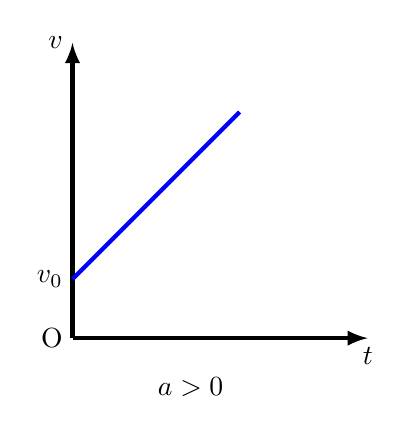
\begin{tikzpicture}[scale=0.75]  
			\coordinate (O) at(0,0);
			\coordinate (x) at(5,0);
			\coordinate (y) at(0,5);
			\coordinate (v0) at(0,1);
			\draw[-latex, line width=1.5pt] (O)--(x);
			\draw[-latex, line width=1.5pt] (O)--(y);
			\draw[blue, line width=1.5pt] (v0)--+(45:4);
			\node[below] at(x) {$t$};
			\node[left] at(y) {$v$};
			\node[left] at(v0) {$v_0$};
			\node[left] at(O) {O};
			\node[below] at (2,-0.5) {$a>0$};
		\end{tikzpicture}
		&
		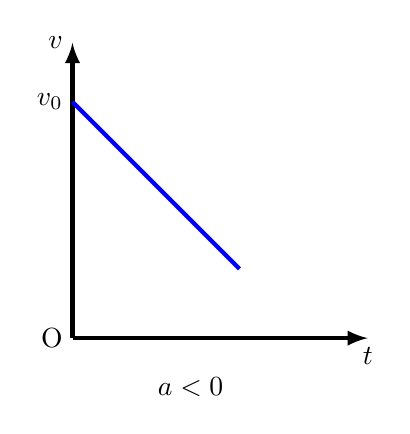
\begin{tikzpicture}  [scale=0.75] 
			\coordinate (O) at(0,0);
			\coordinate (x) at(5,0);
			\coordinate (y) at(0,5);
			\coordinate (v0) at(0,4);
			\draw[-latex, line width=1.5pt] (O)--(x);
			\draw[-latex, line width=1.5pt] (O)--(y);
			\draw[blue, line width=1.5pt] (v0)--+(-45:4);
			\node[below] at(x) {$t$};
			\node[left] at(y) {$v$};
			\node[left] at(v0) {$v_0$};
			\node[left] at(O) {O};
			\node[below] at (2,-0.5) {$a<0$};
		\end{tikzpicture}
	\end{tabular}
\end{center}
\item \textbf{\textit{Vận dụng độ thị vận tốc – thời gian để tính độ dịch chuyển}}\\
\begin{center}
	\begin{tabular}{M{8cm}M{8cm}}
		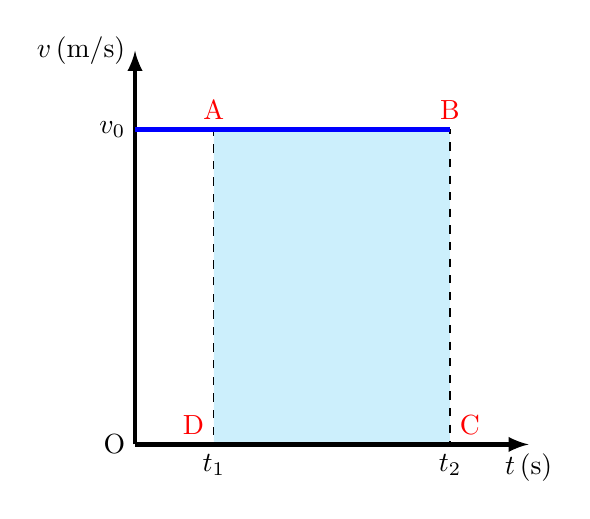
\begin{tikzpicture}  
			\coordinate (O) at(0,0);
			\coordinate (x) at(5,0);
			\coordinate (y) at(0,5);
			\coordinate (v0) at(0,4);
			\coordinate (A) at(1,4);
			\coordinate (B) at(4,4);
			\coordinate (C) at(4,0);
			\coordinate (D) at(1,0);
			\draw[-latex, line width=1.5pt] (O)--(y);
			\fill[cyan, opacity=0.2] (A)--(B)--(C)--(D)--(A);
			\draw[line width=0.5pt,black, dashed] (A)--(B)--(C)--(D)--(A);
			\draw[-latex, line width=1.5pt] (O)--(x);
			\draw[blue, line width=1.5pt] (v0)--(B);
			\node[below] at(x) {$\xsi{t}{\left(\second\right)}$};
			\node[left] at(y) {$\xsi{v}{(\meter/\second)}$};
			\node[left] at(v0) {$v_0$};
			\node[left] at(O) {O};
			\node[below] at (C) {$t_2$};
			\node[below] at (D) {$t_1$};
			\node[above, red] at(A) {A};
			\node[above, red] at(B) {B};
			\node[above right, red] at(C) {C};
			\node[above left, red] at(D) {D};
		\end{tikzpicture}
		&
		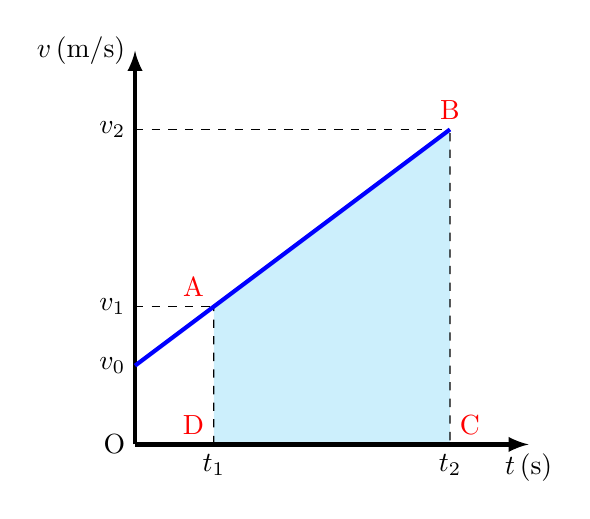
\begin{tikzpicture}  
			\coordinate (O) at(0,0);
			\coordinate (x) at(5,0);
			\coordinate (y) at(0,5);
			\coordinate (v0) at(0,1);
			\coordinate (v1) at(0,1.75);
			\coordinate (v2) at(0,4);
			\coordinate (B) at(4,4);
			\coordinate (A) at(1,1.75);
			\coordinate (C) at(4,0);
			\coordinate (D) at(1,0);
			\fill[cyan, opacity=0.2] (A)--(B)--(C)--(D)--(A);
			\draw[line width=0.5pt,black, dashed] (A)--(B)--(C)--(D)--(A);
			\draw[line width=0.5pt, dashed] (v1)--(A);
			\draw[line width=0.5pt, dashed] (v2)--(B);
			\draw[-latex, line width=1.5pt] (O)--(x);
			\draw[-latex, line width=1.5pt] (O)--(y);
			\draw[blue, line width=1.5pt] (v0)--(B);
			\node[below] at(x) {$\xsi{t}{\left(\second\right)}$};
			\node[left] at(y) {$\xsi{v}{(\meter/\second)}$};
			\node[left] at(v0) {$v_0$};
			\node[left] at(v1) {$v_1$};
			\node[left] at(0,4) {$v_2$};
			\node[left] at(O) {O};
			\node[below] at (C) {$t_2$};
			\node[below] at (D) {$t_1$};
			\node[above left, red] at(A) {A};
			\node[above, red] at(B) {B};
			\node[above right, red] at(C) {C};
			\node[above left, red] at(D) {D};
		\end{tikzpicture}\\
	Đồ thị $v-t$ trong chuyển động\newline thẳng đều. & Đồ thị $v-t$ trong chuyển động \newline thẳng biến đổi đều.
	\end{tabular}
\end{center}
Độ dịch chuyển của vật trong khoảng thời gian từ $t_1$ đến $t_2$ được xác định bằng phần diện tích giới hạn bởi các đường $v\left(t\right)$, $v=0$ , $t=t_1$, $t=t_2$  trong đồ thị $\left(v-t\right)$.
\end{enumerate}
\item \textbf{Các phương trình của chuyển động thẳng biến đổi đều}\\
\begin{itemize}[topsep=0pt]
	\item Phương trình gia tốc: $a=const$;
	\item Phương trình vận tốc: $v=v_0+at$ với $v=v_0$ khi $t_0=0$;
	\item Phương trình quãng đường: $s=v_0t+\dfrac{1}{2}at^2$;
	\item Phương trình toạ độ: $x=x_0+v_0t+\dfrac{1}{2}at^2$;
	\item Phương trình độc lập thời gian:
	$v^2-v^2_0=2as$.
\end{itemize}
\end{enumerate}
\subsection{CÁC  HỒ SƠ KHÁC}
Phiếu học tập\newpage
\textbf{* Phiếu số 1:} Tìm hiểu khái niệm và ý nghĩa của gia tốc.
\begin{center}
	\begin{longtable}{|L{8.5cm}L{8.5cm}|}
		\hline
		\multicolumn{2}{|c|}{\thead{PHIẾU HỌC TẬP SỐ 1 (NHÓM LỚN)\\	TÌM HIỂU KHÁI NIỆM VÀ Ý NGHĨA GIA TỐC
		}}\\
	\hline
	Lớp: \dotfill & Nhóm: \dotfill\\
	\multicolumn{2}{|l|}{Tên: \dotfill}\\
	\hline
	\multicolumn{2}{|L{17cm}|}{\textbf{Nhiệm vụ:} Trong mỗi tình huống sau đây, hãy chỉ ra đối tượng có khả năng tăng tốc hiệu quả hơn (khả năng tăng tốc nhanh hơn) và đưa ra lời giải thích cho lựa chọn của em?}\\
	\hline
	\multicolumn{2}{|c|}{\textbf{Tình huống 1}}\\
	\multicolumn{2}{|L{17cm}|}{
		\begin{itemize}[topsep=0pt]
			\item Báo guépard có khả năng tăng tốc từ $\SI{0}{\kilo\meter/\hour}$ lên $\SI{96}{\kilo\meter/\hour}$ trong thời gian $\SI{3}{\second}$.
			\item Xe đua F1 có khả năng tăng tốc từ $\SI{0}{\meter/\second}$  lên $\SI{25}{\meter/\second}$  trong khoảng thời gian $\SI{3}{\second}$.
		\end{itemize}	
	\dotfill
	}\\
\multicolumn{2}{|L{17cm}|}{
	\dotfill
}\\

\multicolumn{2}{|L{17cm}|}{
	\dotfill
}\\
\hline
\multicolumn{2}{|c|}{\textbf{Tình huống 2}}\\
\multicolumn{2}{|L{17cm}|}{
	\begin{itemize}[topsep=0pt]
		\item Xe Porsche 911 Turbo S Lightweight 2021 có khả năng tăng tốc từ  $\SI{0}{\kilo\meter/\hour}$ lên $\SI{96}{\kilo\meter/\hour}$  trong thời gian $\SI{2.1}{\second}$.
		\item Xe Lamborghini Huracan Performante có khả năng tăng tốc từ $\SI{0}{\kilo\meter/\hour}$  lên $\SI{96}{\kilo\meter/\hour}$  trong thời gian $\SI{2.2}{\second}$.
	\end{itemize}	
	\dotfill
}\\
\multicolumn{2}{|L{17cm}|}{
	\dotfill
}\\

\multicolumn{2}{|L{17cm}|}{
	\dotfill
}\\
\hline
\multicolumn{2}{|c|}{\textbf{Tình huống 3}}\\
\multicolumn{2}{|L{17cm}|}{
	\begin{itemize}[topsep=0pt]
		\item Vận động viên A từ khi xuất phát đến khi đạt tốc độ $\SI{9}{\meter/\second}$  mất thời gian $\SI{2}{\second}$.
		\item Vận động viên B từ khi xuất phát đến khi đạt tốc độ $\SI{6}{\meter/\second}$  mất thời gian $\SI{1.5}{\second}$.
	\end{itemize}	
	\dotfill
}\\
\multicolumn{2}{|L{17cm}|}{
	\dotfill
}\\

\multicolumn{2}{|L{17cm}|}{
	\dotfill
}\\
\multicolumn{2}{|L{17cm}|}{
	\dotfill
}\\
\hline
	\end{longtable}
\end{center}
\newpage
\textbf{Phiếu số 2:} Vận dụng đồ thị $v-t$ để xác định độ dịch chuyển và gia tốc.
\begin{center}
	\begin{longtable}{|L{8.5cm}|L{8.5cm}|}
		\hline
		\multicolumn{2}{|M{17cm}|}{\bfseries PHIẾU HỌC TẬP SỐ 2 \textit{(NHÓM ĐÔI)}\newline
			VẬN DỤNG ĐỒ THỊ  ĐỂ XÁC ĐỊNH ĐỘ DỊCH CHUYỂN VÀ GIA TỐC
		}\\
	\hline
	\multicolumn{2}{|M{17cm}|}{Lớp: \dotfill}\\
	\multicolumn{2}{|M{17cm}|}{Nhóm: \dotfill}\\
	\multicolumn{2}{|M{17cm}|}{Tên: \dotfill}\\
	\hline
	\multicolumn{2}{|L{17cm}|}{
\textbf{Nhiệm vụ:}	Dựa vào đồ thị $\left(v-t\right)$ của vật chuyển động trong hình, hãy xác định gia tốc và độ dịch chuyển của vật trong các giai đoạn:
\begin{center}
	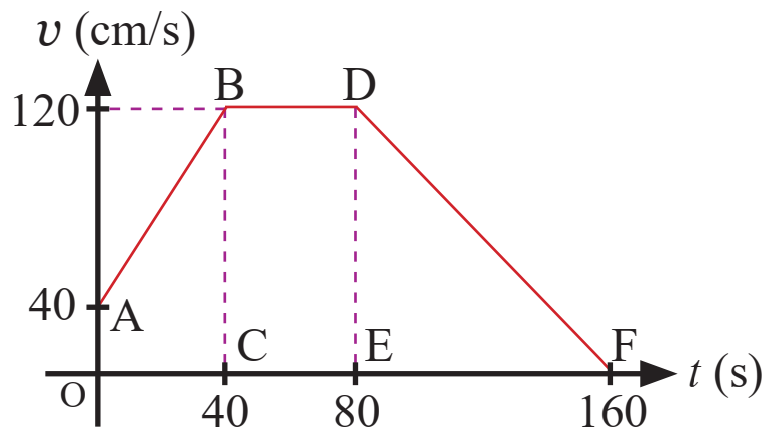
\includegraphics[width=0.4\linewidth]{../figs/BAI7-1}
\end{center}
}\\
a) Từ $\SI{0}{\second}$ đến $\SI{40}{\second}$ & b) Từ $\SI{80}{\second}$ đến $\SI{160}{\second}$\\
\dotfill & \dotfill \\
\dotfill & \dotfill \\
\dotfill & \dotfill \\
\dotfill & \dotfill \\
\dotfill & \dotfill \\
\hline
	\end{longtable}
\end{center}
\newpage
\textbf{Phiếu số 3:} Rút ra được công thức độ dịch chuyển trong chuyển động thẳng biến đổi đều.
\begin{center}
	\begin{longtable}{|L{8.5cm}L{8.5cm}|}
		\hline
	\multicolumn{2}{|L{17cm}|}{\textbf{PHIẾU HỌC TẬP SỐ 3 \textit{(NHÓM LỚN)}	RÚT RA ĐƯỢC CÔNG THỨC ĐỘ DỊCH CHUYỂN TRONG CHUYỂN ĐỘNG THẲNG BIẾN ĐỔI ĐỀU
	}}\\
\hline
Lớp: \dotfill & Nhóm: \dotfill\\
\multicolumn{2}{|L{17cm}|}{Tên: \dotfill}\\
\hline
\multicolumn{2}{|L{17cm}|}{\textbf{Nhiệm vụ:} Dựa vào đồ thị $\left(v-t\right)$ của vật chuyển động thẳng biến đổi đều, hãy rút ra công thức xác định độ dịch chuyển theo $v_0$ , $a$, $t$.
\begin{center}
	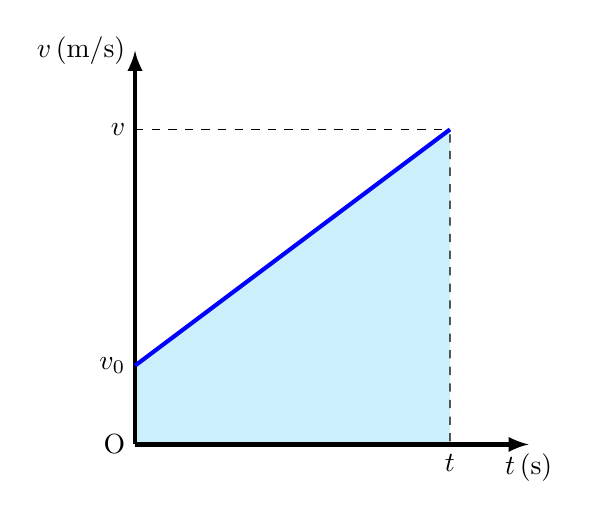
\begin{tikzpicture}  
		\coordinate (O) at(0,0);
		\coordinate (x) at(5,0);
		\coordinate (y) at(0,5);
		\coordinate (v0) at(0,1);
		\coordinate (v1) at(0,1.75);
		\coordinate (v2) at(0,4);
		\coordinate (B) at(4,4);
		\coordinate (A) at(1,1.75);
		\coordinate (C) at(4,0);
		\coordinate (D) at(1,0);
		\fill[cyan, opacity=0.2] (v0)--(B)--(C)--(O)--(v0);
		\draw[line width=0.5pt,black, dashed] (v0)--(B)--(C)--(O)--(v0);
		\draw[line width=0.5pt, dashed] (v2)--(B);
		\draw[-latex, line width=1.5pt] (O)--(x);
		\draw[-latex, line width=1.5pt] (O)--(y);
		\draw[blue, line width=1.5pt] (v0)--(B);
		\node[below] at(x) {$\xsi{t}{\left(\second\right)}$};
		\node[left] at(y) {$\xsi{v}{(\meter/\second)}$};
		\node[left] at(v0) {$v_0$};
		\node[left] at(0,4) {$v$};
		\node[left] at(O) {O};
		\node[below] at (C) {$t$};
	\end{tikzpicture}
\end{center}
}\\
\multicolumn{2}{|L{17cm}|}{\dotfill}\\
\multicolumn{2}{|L{17cm}|}{\dotfill}\\
\multicolumn{2}{|L{17cm}|}{\dotfill}\\
\multicolumn{2}{|L{17cm}|}{\dotfill}\\
\hline
	\end{longtable}
\end{center}
%\chapter{Bài 2. Vấn đề an toàn trong vật lí}
\begin{center}
	\textit{(1 tiết)}
\end{center}
\section{MỤC TIÊU DẠY HỌC}
\begin{center}
	\begin{longtable}{|M{2.5cm}|L{12.5cm}|M{2cm}|}
		\hline
		\thead{Biểu hiện\\ năng lực} & \thead{Mục tiêu} & \thead{STT}\\
		\hline
		\multicolumn{3}{|c|}{\textbf{ Năng lực vật lí}}\\
		\hline
		1.1 & Thảo luận để nêu được các quy tắc an toàn trong nghiên cứu và học tập môn Vật lí & 1\\
		\hline
		\multicolumn{3}{|c|}{\textbf{Năng lực chung}}\\
		\hline
		GT - HT& Tích cực đóng góp ý kiến trong quá trình thảo luận, biết sử dụng ngôn ngữ kết hợp với các loại phương tiện phi ngôn ngữ đa dạng để trình bày các kết quả thảo luận nhóm về các quy tắc an toàn.	& 2\\
		\hline
		
	\end{longtable}
\end{center}
\section{THIẾT BỊ DẠY HỌC VÀ HỌC LIỆU}
\begin{itemize}[topsep=0pt]
	\item SGK.
	\item Phiếu học tập.
\end{itemize}
\section{TIẾN TRÌNH DẠY HỌC}
\subsection{TIẾN TRÌNH}
\begin{center}
	\begin{longtable}{|L{2.75cm}|C{1.25cm}|L{5cm}|L{3.5cm}|L{4cm}|}
		\hline
		\thead{Tiến trình} & \thead{Mục\\tiêu} & \thead{Nội dung dạy học \\trọng tâm} & \thead{PP,\\ KTDH} & \thead{Phương pháp \\đánh giá}\\
		\hline
		\textbf{Hoạt động 1:} Tìm hiểu vấn đề an toàn trong nghiên cứu và học tập vật lí& 1, 2  & Quy tắc an toàn trong nghiên cứu và học tập môn Vật lí  & PP: Dạy học hợp tác.\newline
		KTDH: Kĩ thuật "tia chớp" & GV đánh giá dựa trên kết quả báo cáo thảo luận nhóm của HS.\newline
		PP đánh giá: quan sát, nghe. \\
		\hline
		\textbf{Hoạt động 2:} Luyện tập& 1, 2  & Luyện tập các quy tắc an toàn trong nghiên cứu và học tập môn Vật lí  & PP: Đàm thoại\newline KTDH: Kĩ thuật "tia chớp"& GV đánh giá dựa trên bài tập cá nhân của HS.\newline
		PP đánh giá: quan sát, nghe. \\
		\hline
	\end{longtable}
\end{center}
\subsection{CÁC HOẠT ĐỘNG HỌC}
\hoatdong{Tìm hiểu vấn đề an toàn trong nghiên cứu và học tập vật lí}
{
HS thảo luận để nêu được các quy tắc an toàn trong nghiên cứu và học tập môn vật lí.
}
{Phiếu học tập + Phần trình bày kết quả thảo luận của nhóm HS.

}
{\textit{\underline{* GV chuyển giao nhiệm vụ học tập}}\\
	GV chia lớp thành 4 nhóm. GV yêu cầu các nhóm HS đọc kĩ SGK và thực hiện 2 nhiệm vụ học tập trong phiếu học tập:
	\begin{itemize}
		\item Nhiệm vụ 1: Trình bày những hiểu biết của nhóm về tác hại, lợi ích của chất phóng xạ. Từ đó, nêu những quy tắc an toàn khi làm việc với chất phóng xạ.
		\item Nhiệm vụ 2: Quan sát hình ảnh "Một số tình huống xảy ra trong phòng thí nghiệm", liệt kê những điểm không an toàn trong tình huống.
	\end{itemize}
\textit{\underline{* HS thực hiện nhiệm vụ học tập}}\\
HS: Làm việc theo nhóm được phân công, đọc SGK và thực hiện nhiệm vụ học tập.\\
GV: Theo dõi các nhóm thảo luận để phát hiện kịp thời vấn đề mà nhóm HS gặp phải, từ đó có sự hỗ trợ phù hợp cho mỗi nhóm.\\
\textit{\underline{* HS báo cáo kết quả thực hiện nhiệm vụ học tập}}\\
GV: Yêu cầu 1 nhóm HS trình bày kết quả nhiệm vụ 1. Các nhóm còn lại chú ý theo dõi để nhận xét.\\
HS: Đặt câu hỏi, góp ý.\\
GV: Chỉnh lí, hợp thức hoá kiến thức.\\
GV: Sử dụng kĩ thuật "tia chớp" để các nhóm trình bày kết quả thảo luận nhiệm vụ 2. GV chia bảng thành 4 phần, HS các nhóm thay phiên nhau lên bảng viết các ý thảo luận ở nhiệm vụ 2, mỗi lượt HS lên bảng chỉ được viết 1 ý. Sau thời gian 2 phút, nhóm nào viết được nhiều ý nhất là nhóm chiến thắng.\\
HS: Nhận xét các ý của mỗi nhóm.\\
GV: Chỉnh lí, hợp thức hoá kiến thức.
}
\hoatdong{
Luyện tập
}
{
HS vận dụng quy tắc an toàn trong nghiên cứu và học tập môn vật lí
}
{Bài tập các nhân của HS.

}
{\textit{\underline{* GV chuyển giao nhiệm vụ học tập}}\\
	GV: Khởi đầu hoạt động luyện tập bằng hoạt động hỏi đáp nhanh. GV chiếu một số biển báo cảnh báo cùng một số trang bị bảo hộ thường gặp, yêu cầu HS đáp nhanh ý nghĩa của mỗi biển báo và công dụng của mỗi trang thiết bị bảo hộ trong phòng thí nghiệm.\\
	GV lần lượt chuyển giao từng bài tập, yêu cầu HS hoạt động cá nhân để giải.\\
	\textit{\underline{* HS thực hiện nhiệm vụ học tập}}\\
	HS \textit{(làm việc cá nhân)}:  Giải bài tập trong phiếu bài tập được GV giao. 
	
	GV: Theo dõi để phát hiện các HS gặp khó khăn, từ đó đưa ra sự định hướng, hỗ trợ phù hợp cho mỗi HS.\\
	\textit{\underline{* HS báo cáo kết quả thực hiện nhiệm vụ học tập}}\\
	GV: Mời HS lên bảng giải bài tập.
	
	HS: Đặt câu hỏi, góp ý.
	
	GV: Chỉnh lí, hợp thức hoá kiến thức.

}
\section{HỒ SƠ DẠY HỌC}
\subsection{NỘI DUNG DẠY HỌC}
\begin{enumerate}[label=\bfseries \arabic*.]
	\item \textbf{Chất phóng xạ}
	\begin{enumerate}[label=\alph*/]
		\item Tác hại: Gây tổn thương da, các bệnh ung thư, làm biến đổi gen.
		\item Lợi ích: Dùng trong chẩn đoán và điều trị bệnh, khử trùng thực phẩm, kiểm tra an ninh, kiểm tra chất lượng trong công nghiệp, tạo ra giống cây trồng mới, nghiên cứu khoa học, \dots
		\item Quy tắc an toàn khi làm việc với chất phóng xạ: Sử dụng găng tay và đồ bảo hộ khi thực hiện thí nghiệm, không để chất phóng xạ tiếp xúc trực tiếp với cơ thể, giữ khoảng cách phù hợp, chú ý thời gian tiếp xúc với chất phóng xạ đủ ngắn, quan tâm đến việc che chắn các cơ quan nhạy cảm với chất phóng xạ.
	\end{enumerate}
\item \textbf{An toàn trong thí nghiệm}
\begin{enumerate}[label=\alph*/]
	\item Một số biện pháp an toàn khi sử dụng điện:
	\begin{itemize}
		\item Trang bị đầy đủ các thiết bị bảo hộ cá nhân
		\item Giữ khoảng cách an toàn với nguồn điện
		\item Tránh sử dụng các thiết bị điện khi đang sạc
		\item Không dùng tay ướt hoặc nhiều mồ hôi khi sử dụng dây điện
		\item Tránh xa nơi điện thế nguy hiểm
		\item Lắp đặt vị trí cầu dao, cầu chì, công tắc, ổ điện đúng quy định
	\end{itemize}
\item Khi nghiên cứu và học tập vật lí ta cần phải:
\begin{itemize}
	\item Nắm được thông tin liên quan đến các rủi ro và nguy hiểm có thể xảy ra.
	\item Tuân thủ và áp dụng các biện pháp bảo vệ để đảm bảo an toàn cho bản thân và cộng đồng.
	\item Quan tâm, gìn giữ và bảo vệ môi trường.
	\item Trong phòng thí nghiệm ở trường học, những rủi ro và nguy hiểm phải được cảnh báo rõ ràng bởi các biển báo. Học sinh cần chú ý sự nhắc nhở của nhân viên phòng thí nghiệm và giáo viên về các quy định an toàn. Ngoài ra các thiết bị bảo hộ cá nhân cần phải được trang bị đầy đủ.
\end{itemize}
\end{enumerate}
\end{enumerate}
\subsection{CÁC HỒ SƠ KHÁC}
Phiếu học tập
\begin{center}
	\begin{longtable}{|L{8.5cm}|L{8.5cm}|}
		\hline
		\multicolumn{2}{|c|}{\thead{PHIẾU HỌC TẬP SỐ\\	TÌM HIỂU VẤN ĐỀ AN TOÀN TRONG NGHIÊN CỨU VÀ HỌC TẬP VẬT LÍ
		}}\\
		\hline
		\multicolumn{1}{|L{8.5cm}}{Lớp: \dotfill} & \multicolumn{1}{L{8.5cm}|}{Nhóm: \dotfill}\\
		\multicolumn{2}{|l|}{Tên: \dotfill}\\
		\hline
		\multicolumn{2}{|L{17cm}|}{\textbf{Nhiệm vụ 1:} Trình bày những hiểu biết của em về tác hại và lợi ích của chất phóng xạ. Từ đó, nêu những quy tắc an toàn khi làm việc với chất phóng xạ.}\\
		\hline
		\thead{Lợi ích} & \thead{Tác hại}\\
		\hline
		\dotfill&\dotfill\\
		\dotfill&\dotfill\\
		\dotfill&\dotfill\\
		\dotfill&\dotfill\\
		\dotfill&\dotfill\\
		\dotfill&\dotfill\\
		\hline
		\multicolumn{2}{|L{17cm}|}{\thead{Quy tắc an toàn khi làm việc với chất phóng xạ}}\\
		\multicolumn{2}{|L{17cm}|}{\dotfill}\\
		\multicolumn{2}{|L{17cm}|}{\dotfill}\\
		\multicolumn{2}{|L{17cm}|}{\dotfill}\\
		\multicolumn{2}{|L{17cm}|}{\dotfill}\\
		\hline
		\multicolumn{2}{|L{17cm}|}{\textbf{Nhiệm vụ 2:} Quan sát hình bên dưới và chỉ ra những điểm không an toàn khi làm việc trong phòng thí nghiệm.}\\
		\multicolumn{2}{|M{17cm}|}{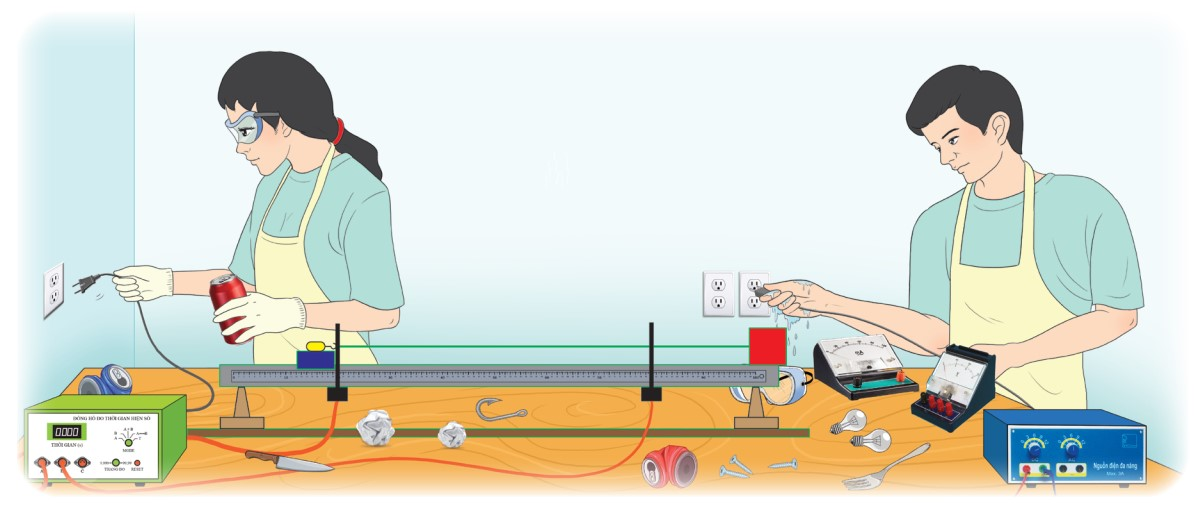
\includegraphics[width=0.8\linewidth]{figs/BAI2-1}}\\
		\multicolumn{2}{|L{17cm}|}{\dotfill}\\
		\multicolumn{2}{|L{17cm}|}{\dotfill}\\
		\multicolumn{2}{|L{17cm}|}{\dotfill}\\
		\multicolumn{2}{|L{17cm}|}{\dotfill}\\
		\hline
	\end{longtable}
\end{center}
Một số biển báo cảnh báo cùng một số trang thiết bị bảo hộ thường gặp.
\begin{center}
	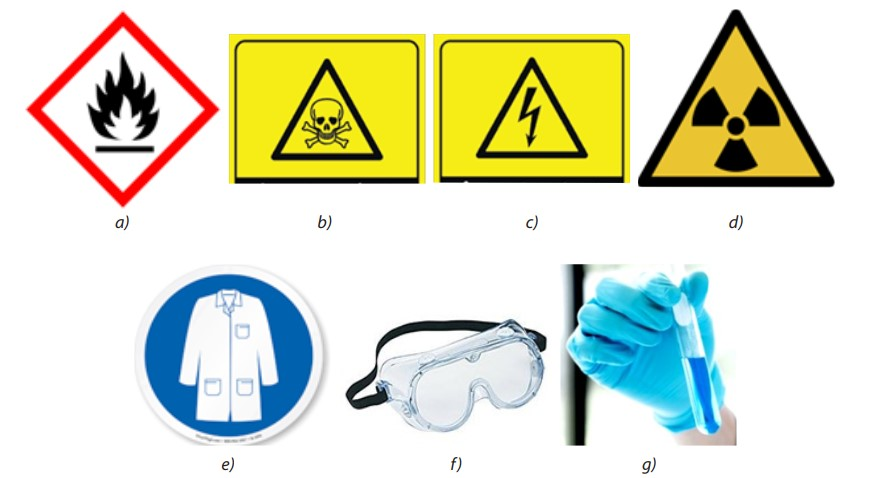
\includegraphics[width=0.8\linewidth]{figs/BAI2-2}
\end{center}
%\chapter{Bài 3. Đơn vị và sai số trong vật lí}
%\begin{center}
%	\textit{(3 tiết)}
%\end{center}
%\section{MỤC TIÊU DẠY HỌC}
%\begin{center}
%	\begin{longtable}{|M{2.5cm}|L{12.5cm}|M{2cm}|}
%		\hline
%		\thead{Biểu hiện\\ năng lực} & \thead{Mục tiêu} & \thead{STT}\\
%		\hline
%		\multicolumn{3}{|c|}{\textbf{ Năng lực vật lí}}\\
%		\hline
%		1.1 & Nêu được hệ đơn vị SI, đơn vị cơ bản, đơn vị dẫn xuất & 1\\
%		\hline
%		1.1& Nêu được khái niệm thứ nguyên & 2\\
%		\hline
%		1.2 & Vận dụng được mối liên hệ giữa đơn vị dẫn xuất với 7 đơn vị cơ bản &3\\
%		\hline
%		1.1 & Thảo luận để nêu được một số loại sai số đơn giản hay gặp khi đo các đại lượng vật lí và cách khắc phục chúng & 4\\
%		\hline
%		1.2 & Biểu diễn được kết quả đo đại lượng vật lí & 5\\
%		\hline
%		1.2 & Xác định được sai số trong phép đo gián tiếp & 6\\
%		\hline
%		\multicolumn{3}{|c|}{\textbf{Năng lực chung}}\\
%		\hline
%		TC - TH& Tích cực thực hiện các nhiệm vụ GV đặt ra cho các nhóm, tích cực suy luận để đưa ra câu trả lời trong quá trình GV định hướng nội dung học tập	&7 \\
%		\hline
%		GT - HT & Tích cực đóng góp ý kiến trong quá trình thảo luận, biết sử dụng ngôn ngữ kết hợp với các loại phương tiện phi ngôn ngữ đa dạng để trình bày các kết quả thảo luận nhóm & 8\\
%		\hline
%	\end{longtable}
%\end{center}
%\section{THIẾT BỊ DẠY HỌC VÀ HỌC LIỆU}
%\begin{itemize}
%	\item Tivi/máy chiếu;
%	\item SGK;
%	\item Phiếu học tập.
%\end{itemize}
%\section{TIẾN TRÌNH DẠY HỌC}
%\subsection{TIẾN TRÌNH}\newpage
%\begin{center}
%	\begin{longtable}{|L{2.75cm}|C{1.25cm}|L{5cm}|L{3.5cm}|L{4cm}|}
%		\hline
%		\thead{Tiến trình} & \thead{Mục\\tiêu} & \thead{Nội dung dạy học \\trọng tâm} & \thead{PP,\\ KTDH} & \thead{Phương pháp \\đánh giá}\\
%		\hline
%		\textbf{Hoạt động 1:} Tìm hiểu đơn vị và thứ nguyên trong vật lí&1, 2  & Hệ đơn vị SI, đơn vị cơ bản và đơn vị dẫn xuất, thứ nguyên  & PP: Đàm thoại\newline
%		KTDH: Kĩ thuật "tia chớp"  & GV đánh giá dựa trên câu trả lời của HS.\newline
%		PP đánh giá: quan sát, nghe. \\
%		\hline
%		\textbf{Hoạt động 2:} Vận dụng mối liên hệ giữa đơn vị dẫn xuất và đơn vị cơ bản & 3, 7, 8 & Mối liên hệ giữa đơn vị dẫn xuất và đơn vị cơ bản & PP: Dạy học hợp tác\newline
%		KTDH: Kĩ thuật "các mảnh ghép" & GV đánh giá dựa trên thái độ của HS trong các nhóm và kết quả thảo luận nhóm.\newline PP đánh giá: quan sát, nghe.\\
%		\hline
%		\textbf{Hoạt động 3:} Tìm hiểu sai số trong phép đo và cách hạn chế & 4, 7, 8 & Các phép đo, các loại sai số trong vật lí & PP: Dạy học hợp tác.\newline
%		KTDH: Đọc tích cực, chia sẻ cặp đôi & GV đánh giá dựa trên câu trả và phiếu học tập nhóm đôi của HS.\newline PP đánh giá: quan sát, nghe.\\
%		\hline
%		\textbf{Hoạt động 4:} Tìm hiểu cách biểu diễn sai số của phép đo & 5, 6, 7, 8 & Cách biểu diễn kết quả đo trực tiếp, cách xác định sai số trong phép đo gián tiếp & PP: Đàm thoại.\newline KTDH: kĩ thuật "chia sẻ cặp đôi" & GV đánh giá dựa trên phiếu học tập của HS.\newline
%		PP đánh giá: quan sát, nghe.\\
%		\hline
%		\textbf{Hoạt động 5:} Luyện tập & 1 - 6 & Luyện tập bài tập xác định CSCN, xác định sai số trong phép đo trực tiếp, sai số trong phép đo gián tiếp & PP: Đàm thoại. & GV đánh giá dựa trên bài tập cá nhân của HS\newline
%		PP đánh giá: quan sát, nghe.\\
%		\hline
%	\end{longtable}
%\end{center}
%\subsection{CÁC HOẠT ĐỘNG HỌC}
%\hoatdong{Tìm hiểu đơn vị và thứ nguyên trong vật lí
%}
%{
%HS nêu được hệ đơn vị SI, đơn vị cơ bản và đơn vị dẫn xuất.
%
%HS nêu được thứ nguyên của các đại lượng vật lí, phân biệt được thứ nguyên với đơn vị.
%}
%{
%Câu trả lời của HS.
%}
%{
%\textit{\underline{* GV chuyển giao nhiệm vụ học tập}}\\
%GV dẫn dắt vào bài. GV sử dụng kĩ thuật "tia chớp" yêu cầu HS kể tên một số đại lượng vật lí và đơn vị của chúng mà HS đã được học trong môn KHTN.\\
%GV giới thiệu về hệ đơn vị SI, các đơn vị cơ bản, tên và kí hiệu tiếp đầu ngữ của bội số, ước số thập phân của đơn vị.\\
%GV giới thiệu khái niệm thứ nguyên, cách xác định thứ nguyên của đại lượng vật lí, nguyên tắc về thứ nguyên trong 1 biểu thức vật lí.\\
%GV lấy ví dụ hướng dẫn học sinh xác định thứ nguyên của tốc độ.\\
%\textit{\underline{* HS thực hiện nhiệm vụ học tập}}\\
%HS tích cực trả lời câu hỏi gợi mở của GV.\\
%HS chú ý theo dõi, đặt câu hỏi.
%}
%% ===============================================================
%\hoatdong{Vận dụng mối liên hệ giữa đơn vị dẫn xuất và đơn vị cơ bản}
%{
%HS vận dụng được mối liên hệ giữa đơn vị dẫn xuất với 7 đơn vị cơ bản của hệ SI.
%}
%{
%Phiếu học tập 1.
%}
%{\textit{\underline{* GV chuyển giao nhiệm vụ học tập}}\\
%	GV hướng dẫn HS thực hiện ví dụ trong SGK trang 17 mục "Vận dụng mối liên hệ giữa đơn vị dẫn xuất với 7 đơn vị cơ bản của hệ SI".\\
%	GV sử dụng kĩ thuật "các mảnh ghép" cho HS thực hiện hoạt động học tập 2:
%	\begin{itemize}
%		\item \textbf{Vòng 1:} GV chia lớp thành 6 nhóm, mỗi nhóm gồm  2 bàn quay lại với nhau. GV phân công nhóm 1 + 4 thực hiện nhiệm vụ 1; nhóm 2 + 5 thực hiện nhiệm vụ 2; nhóm 3 + 6 thực hiện nhiệm vụ 3 trong phiếu học tập 1. GV yêu cầu các nhóm thảo luận tích cực và đảm bảo mỗi thành viên đều nắm được kết quả thảo luận của nhóm. Trong mỗi nhóm, GV đánh STT các thành viên từ 1 đến 6. Hoạt động vòng 1 diễn ra trong 10 phút. Các nhóm ghi lại kết quả thảo luận vào phiếu học tập của nhóm để nộp lại cho GV.
%		\item \textbf{Vòng 2:} GV yêu cầu các HS có cùng STT di chuyển về 1 nhóm. Các HS lần lượt trao đổi với các thành viên còn lại trong nhóm về kết quả thảo luận ở vòng 1. Các nhóm thảo luận tích cực và đảm bảo rằng các thành viên trong nhóm đều nắm được kết quả của 3 nhiệm vụ học tập. Các nhóm thống nhất trình bày kết quả 3 nhiệm vụ vào biên bản chung để nộp cho GV. Hoạt động vòng 2 diễn ra trong 15 phút.
%	\end{itemize}
%\textit{\underline{* HS thực hiện nhiệm vụ học tập}}\\
%HS hoạt động theo nhóm được phân công, tích cực thảo luận.\\
%Trong quá trình di chuyển, HS trật tự và đi theo hướng dẫn của GV.\\
%\textit{\underline{* HS báo cáo kết quả thực hiện nhiệm vụ học tập}}\\
%GV chọn đại diện của 3 nhóm HS bất kì lên bảng trình bày kết quả thảo luận.\\
%HS chú ý theo dõi, nhận xét phần trình bày của các nhóm.\\
%GV chỉnh lí, hợp thức hoá kiến thức.
%
%}
%% ========================================================
%\hoatdong{
%	Tìm hiểu sai số trong phép đo và cách hạn chế
%}
%{
%	HS nêu được một số loại sai số đơn giản hay gặp khi đo các đại lượng vật lí.\\
%	HS nêu được giải pháp hạn chế một số loại sai số đơn giản hay gặp khi đo các đại lượng vật lí.
%}
%{
%Phiếu học tập 2
%}
%{\textit{\underline{* GV chuyển giao nhiệm vụ học tập}}\\
%	GV yêu cầu HS hoạt động theo nhóm 2 hoặc nhóm 3 HS.\\
%	GV yêu cầu các nhóm nghiên cứu SGK mục "Các phép đo trong vật lí" và "Các loại sai số của phép đo" để hoàn thành 2 bảng so sánh trong phiếu học tập 2.\\
%	\textit{\underline{* HS thực hiện nhiệm vụ học tập}}\\
%	HS hoạt động theo nhóm được chia, đọc tích cực và hoàn thành bảng so sánh ở phiếu học tập 2.\\
%	GV theo dõi hoạt động của các nhóm, hỗ trợ khi HS gặp khó khăn.\\
%	\textit{\underline{* HS báo cáo kết quả thực hiện nhiệm vụ học tập}}\\
%	GV lần lượt mời các nhóm bất kì điền kết quả vào bảng so sánh.\\
%	HS theo dõi, nhận xét, đặt câu hỏi.\\
%	GV chỉnh lí, hợp thức hoá kiến thức.
%
%}
%% ===========================================================
%\hoatdong{
%Tìm hiểu cách biểu diễn sai số của phép đo
%}
%{
%HS xác định được sai số trong phép đo trực tiếp và phép đo gián tiếp.\\
%HS biểu diễn được kết quả đo đại lượng vật lí.
%}
%{Bài tập vận dụng xác định sai số trong phép đo trực tiếp và sai số trong phép đo gián tiếp
%
%}
%{\textit{\underline{* GV chuyển giao nhiệm vụ học tập}}\\
%	GV giới thiệu cho HS các khái niệm: giá trị trung bình, sai số tuyệt đối, sai số tương đối.\\
%	GV hướng dẫn HS cách biểu diễn sai số của phép đo trực tiếp, cách xác định số CSCN và quy tắc làm tròn số.\\
%	GV dẫn dắt cho HS làm bài tập vận dụng 1 ở Bảng 3.4 SGK CTST trang 22.\\
%	GV hướng dẫn HS cách xác định sai số gián tiếp.\\
%	GV dẫn dắt HS thực hiện bài tập vận dụng 2 trang 22.\\
%	\textit{\underline{* HS thực hiện nhiệm vụ học tập}}\\
%	HS chú ý lắng nghe phần hướng dẫn của GV và đặt câu hỏi (nếu có).\\
%	HS thực hiện bài tập vận dụng 1 và vận dụng 2.\\
%	\textit{\underline{* HS báo cáo kết quả thực hiện nhiệm vụ học tập}}\\
%	GV mời HS trả lời trong quá trình hướng dẫn bài tập vận dụng 1 và vận dụng 2.\\
%	GV chỉnh lí, hợp thức hoá kiến thức.
%}
%%%%%%%%%%%%%%%%%%%%%%%%%%%%%%%%%%%%%%%%%%%%%%
%\hoatdong{
%	Luyện tập.
%}
%{
%	HS xác định được số CSCN, sai số trong phép đo trực tiếp, sai số trong phép đo gián tiếp.
%}
%{
%	Bài tập cá nhân của học sinh.
%}
%{
%	\textit{\underline{GV chuyển giao nhiệm vụ học tập}}\\
%	GV lần lượt chuyển giao từng bài tập, yêu cầu HS hoạt động cá nhân để giải.\\
%	\textit{\underline{HS thực hiện nhiệm vụ học tập}}\\
%	HS \textit{(làm việc cá nhân)}:  Giải bài tập trong phiếu bài tập được GV giao. 
%	
%	GV: Theo dõi để phát hiện các HS gặp khó khăn, từ đó đưa ra sự định hướng, hỗ trợ phù hợp cho mỗi HS.\\
%	\textit{\underline{HS báo cáo kết quả thực hiện nhiệm vụ học tập}}\\
%	GV: Mời HS lên bảng giải bài tập.
%	
%	HS: Đặt câu hỏi, góp ý.
%	
%	GV: Chỉnh lí, hợp thức hoá kiến thức.
%}
%
%\section{HỒ SƠ DẠY HỌC}
%\subsection{NỘI DUNG DẠY HỌC}
%\begin{enumerate}[label=\bfseries\Roman*.]
%	\item \textbf{ĐƠN VỊ VÀ THỨ NGUYÊN TRONG VẬT LÍ}\\
%	Trong khoa học có rất nhiều hệ đơn vị được sử dụng, trong đó thông dụng nhất là hệ đơn vị đo lường quốc tế SI (Système International d’unités) được xây dựng trên cơ sở của 7 đơn vị cơ
%	bản.
%	\begin{enumerate}[label=\bfseries\arabic*.]
%		\item \textbf{Các đơn vị cơ bản trong hệ SI}
%		\begin{center}
%			\begin{longtable}{|M{1.5cm}|M{3cm}|M{3cm}|M{4cm}|}
%				\hline
%				\thead{STT}&\thead{Đơn vị}& \thead{Kí hiệu} &\thead{Đại lượng}\\
%				\hline
%				1 & mét & $\si{\meter}$ & Chiều dài\\
%				\hline
%				2 & kilogram & $\si{\kilogram}$ & Khối lượng \\
%				\hline
%				3 & giây & $\si{\second}$ & Thời gian \\
%				\hline
%				4 & kelvin & $\si{\kelvin}$ & Nhiệt độ \\
%				\hline
%				5 & ampere & $\si{\ampere}$ & Cường độ dòng điện\\
%				\hline
%				6 & mol & $\si{\mole}$ & Lượng chất\\
%				\hline
%				7 & candela & $\si{\candela}$ &  Cường độ sáng\\
%				\hline
%			\end{longtable}
%		\end{center}
%	Ngoài 7 đơn vị cơ bản, những đơn vị còn lại được gọi là \textbf{đơn vị dẫn xuất}.
%	\item \textbf{Tên và kí hiệu tiếp đầu ngữ của bội số, ước số thập phân của đơn vị}
%	\begin{center}
%		\newcolumntype{a}[1]{>{\centering\arraybackslash\columncolor{gray}}p{#1}}
%		\begin{longtable}{|M{2cm}|M{2cm}|M{2cm}|a{0.5cm}|M{2cm}|M{2cm}|M{2cm}|}
%			\hline
%			\thead{Kí hiệu}&\thead{Tên đọc}& \thead{Hệ số}&&\thead{Kí hiệu}&\thead{Tên đọc}&\thead{Hệ số}\\
%			\hline
%			Y &yotta& $10^{24}$&&y & yokto &$10^{-24}$\\ 
%			\hline
%			Z &zetta& $10^{21}$&&z & zepto &$10^{-21}$\\ 
%			\hline
%			E &eta& $10^{18}$&&a & atto &$10^{-18}$\\ 
%			\hline
%			P &peta& $10^{15}$&&f & femto &$10^{-15}$\\ 
%			\hline
%			T &tera& $10^{12}$&&p & pico &$10^{-12}$\\ 
%			\hline
%			G &giga& $10^{9}$&&n & nano &$10^{-9}$\\ 
%			\hline
%			M &mega& $10^{6}$&&$\mathnormal{\mu}$ & micro &$10^{-6}$\\ 
%			\hline
%			k &kilo& $10^{3}$&&m & milli &$10^{-3}$\\ 
%			\hline
%			h &hecto& $10^{2}$&&c & centi &$10^{-2}$\\ 
%			\hline
%			da &deka& $10^{1}$&&d & deci &$10^{-1}$\\ 
%			\hline
%		\end{longtable}
%	\end{center}
%\item \textbf{Thứ nguyên}\\
%Thứ nguyên của một đại lượng là quy luật nêu lên sự phụ thuộc của đơn vị đo đại lượng đó vào các đơn vị cơ bản. Thứ nguyên của một đại lượng X được biểu diễn dưới dạng $\left[X\right]$.\\
%\textbf{Thứ nguyên của một số đại lượng cơ bản}:
%\begin{center}
%	\begin{longtable}{|M{6cm}|M{6cm}|}
%		\hline
%		\thead{Đại lượng cơ bản}&\thead{Thứ nguyên}\\
%		\hline
%		[Chiều dài] & L\\
%		\hline
%		[Khối lượng] & M\\
%		\hline
%		[Thời gian] & T\\
%		\hline
%		[Cường độ dòng điện] & I\\
%		\hline
%		[Nhiệt độ]&K\\
%		\hline
%	\end{longtable}
%\end{center}
%\textbf{Ví dụ:} Tọa độ, quãng đường có thứ nguyên là L; vận tốc có thứ nguyên là $L\cdot T^{-1}$; khối lượng riêng có thứ nguyên là $M\cdot L^{-3}$,\dots\\
%\textbf{Lưu ý:} Trong các biểu thức vật lí:
%\begin{itemize}
%	\item Các số hạng trong phép cộng (hoặc trừ) phải có cùng thứ
%	nguyên.
%	\item Hai vế của một biểu thức vật lí phải có cùng thứ nguyên.
%\end{itemize}
%\item \textbf{SAI SỐ TRONG PHÉP ĐO VÀ CÁCH HẠN CHẾ}\\
%\begin{enumerate}[label=\bfseries\arabic*.]
%	\item \textbf{Các phép đo trong vật lí}
%	\begin{itemize}
%		\item Phép đo các đại lượng vật lí là phép so sánh chúng với đại lượng cùng loại được quy ước làm đơn vị.
%		\item \textit{Phép đo trực tiếp}: giá trị của đại lượng cần đo được đọc trực tiếp trên dụng cụ đo (ví dụ như đo khối lượng bằng cân, đo thể tích bằng bình chia độ).
%		\item \textit{Phép đo gián tiếp}: giá trị của đại lượng cần đo được xác định thông qua các đại lượng được đo trực tiếp (ví dụ như đo khối lượng riêng).
%	\end{itemize}
%\item \textbf{Các loại sai số của phép đo}\\
%\begin{enumerate}[label=\bfseries\alph*)]
%	\item \textbf{Sai số hệ thống:} là sai số có tính quy luật và được lặp lại ở tất cả các lần đo. Sai số hệ thống làm cho giá trị đo tăng hoặc giảm một lượng nhất định so với giá trị thực.\\
%	Sai số hệ thống thường xuất phát từ dụng cụ đo (ví dụ: không
%	hiệu chỉnh dụng cụ về đúng số 0, \dots). Ngoài ra sai số hệ thống còn xuất phát từ độ chia nhỏ nhất của dụng cụ đo (gọi là sai số dụng cụ, thường được xác định bằng một nửa độ chia nhỏ nhất).\\
%	$\Rightarrow$ Sai số hệ thống có thể hạn chế bằng cách hiệu chỉnh dụng cụ trước khi đo, lựa chọn dụng cụ đo phù hợp, thao tác đo đúng cách.
%	\item \textbf{Sai số ngẫu nhiên:} là sai số xuất phát từ sai sót, phản xạ của người làm thí nghiệm hoặc từ những yếu tố ngẫu nhiên bên ngoài. Sai số này thường có nguyên nhân không rõ ràng và dẫn đến sự phân tán của các kết quả đo xung quanh một giá trị trung bình.\\
%	Sai số ngẫu nhiên có thể được hạn chế bằng cách: thực hiện phép đo nhiều lần và lấy giá trị trung bình để hạn chế sự phân tán
%	của số liệu đo.
%\end{enumerate}
%\item \textbf{Cách biểu diễn sai số của phép đo}\\
%Khi tiến hành đo đạc, giá trị $x$ của một đại lượng vật lí thường được ghi dưới dạng
%$$x=\overline{x}+\Delta x$$
%với $\overline{x}$ là giá trị trung bình của đại lượng cần đo khi tiến hành phép đo nhiều lần:
%$$\overline{x}=\dfrac{x_1+x_2+\dots+x_n}{n}$$
%Sai số của phép đo được biểu diễn dưới dạng:
%\begin{itemize}
%	\item \textbf{Sai số tuyệt đối} $\Delta x$:
%	\begin{itemize}
%		\item Sai số tuyệt đối ứng với mỗi lần đo được xác định bằng trị tuyệt đối của hiệu giữa giá trị trung bình và giá trị của mỗi lần đo
%		$$\Delta x_i=\left|\overline{x}-x_i\right|$$
%		với $x_i$ là giá trị lần đo thứ $i$.
%		\item Sai số tuyệt đối trung bình của $n$ lần đo được xác định theo công thức
%		$$\overline{\Delta x}=\dfrac{\Delta x_1+\Delta x_2+\dots+\Delta x_n}{n}$$
%		\item Sai số tuyệt đối của phép đo cho biết phạm vi biến thiên của giá trị đo được và bằng tổng của sai số ngẫu nhiên và sai số dụng cụ:
%		$$\Delta x=\overline{\Delta x}+\Delta x_{\text{dc}}$$
%		Trong đó sai số dụng cụ $\Delta x_{\text{dc}}$ thường được xem có giá trị bằng một nửa độ chia nhỏ nhất với những dụng cụ đơn giản như thước kẻ, cân bàn, bình chia độ, \dots
%	\end{itemize}
%\item \textbf{Sai số tương đối:} được xác định bằng tỉ số giữa sai số tuyệt đối và giá trị trung bình của đại lượng cần đo theo công thức:
%$$\delta x=\dfrac{\Delta x}{\overline{x}}\cdot\SI{100}{\percent}$$
%Sai số tương đối cho biết mức độ chính xác của phép đo.
%\end{itemize}
%\item \textbf{Cách xác định sai số trong phép đo gián tiếp}\\
%Nguyên tắc xác định sai số trong phép đo gián tiếp như sau:
%\begin{itemize}
%	\item Sai số tuyệt đối của một tổng hay hiệu bằng tổng sai số tuyệt đối của các số hạng:\\
%	Nếu $F=x\pm y\pm z\pm\dots$ thì $\Delta F=\Delta x+\Delta y+\Delta z+\dots$
%	\item Sai số tương đối của một tích hoặc thương bằng tổng sai số tương đối của các thừa số:\\
%	Nếu $F=x^m\dfrac{y^n}{z^k}$ thì $\delta F=m\cdot\delta x+n\cdot\delta y+k\cdot\delta z$.\\
%	\textbf{\textit{Các chữ số có nghĩa gồm:}} Các chữ số khác 0, các chữ số 0 nằm giữa hai chữ số khác 0 hoặc nằm bên phải của dấu thập phân và một chữ số khác 0.\\
%	\textbf{Ví dụ:} 765 có ba chữ số có nghĩa, 7005 có bốn chữ số có nghĩa, 0,0700 có ba chữ số có nghĩa.
%\end{itemize}
%\end{enumerate}
%
%	\end{enumerate}
%\end{enumerate}
%\subsection{CÁC HỒ SƠ KHÁC}
%\newpage
%* Phiếu học tập 1
\begin{center}
	\begin{longtable}{|M{8.5cm}|M{8.5cm}|}
		\hline
		\multicolumn{2}{|c|}{\thead{PHIẾU HỌC TẬP  \\	VẬN DỤNG MỐI LIÊN HỆ GIỮA ĐƠN VỊ DẪN XUẤT VÀ ĐƠN VỊ CƠ BẢN
		}}\\
		\hline
		\multicolumn{1}{|L{8.5cm}}{Lớp: \dotfill} & \multicolumn{1}{L{8.5cm}|}{Nhóm: \dotfill}\\
		\multicolumn{2}{|L{17cm}|}{Tên: \dotfill}\\
		\hline
		\multicolumn{2}{|L{17cm}|}{\textbf{Nhiệm vụ 1:} Em hãy phân tích thứ nguyên của các đại lượng vật lí sau đây\newline
	\textit{* Gợi ý: Thứ nguyên của lực là $M\cdot L\cdot T^{-2}$.}	
	}\\
		\multicolumn{2}{|M{17cm}|}{
	\begin{center}
		\begin{tabular}{|M{8cm}|M{8cm}|}
			\hline
			\thead{Đại lượng} & \thead{Thứ nguyên}\\
			\hline
			Khối lượng riêng & \\
			\hline
			Công & \\
			\hline
			Công suất &\\
			\hline
			Áp suất & \\
			\hline
		\end{tabular}
	\end{center}	
	}\\
\hline
\multicolumn{
2
}{|L{17cm}|}{\textbf{Nhiệm vụ 2:} Tốc độ truyền sóng $v$ trên một sợi dây đàn hồi phụ thuộc vào lực căng $F$ và mật độ khối lượng $\mu$ (khối lượng trên một đơn vị chiều dài) của sợi dây. Bằng việc phân tích thứ nguyên, một bạn học sinh thiết lập biểu thức $v$ theo $F$ và $\mu$ như sau:
$$v=\alpha\cdot\dfrac{F}{\mu}$$
với $\alpha$ là hằng số không thứ nguyên. Công thức bạn học sinh đưa ra có phù hợp nguyên tắc thứ nguyên không?\newline
\textit{* Gợi ý: Thứ nguyên của lực là $M\cdot L\cdot T^{-2}$.}	
}\\
\multicolumn{2}{|L{17cm}|}{\dotfill}\\
\multicolumn{2}{|L{17cm}|}{\dotfill}\\
\multicolumn{2}{|L{17cm}|}{\dotfill}\\
\multicolumn{2}{|L{17cm}|}{\dotfill}\\
\multicolumn{2}{|L{17cm}|}{\dotfill}\\
\multicolumn{2}{|L{17cm}|}{\dotfill}\\
\hline
\multicolumn{2}{|L{17cm}|}{\textbf{Nhiệm vụ 3:} Lực cản không khí tác dụng lên vật phụ thuộc vào tốc độ chuyển động của vật theo công thức $F=-kv^2$. Biết thứ nguyên của lực là $M\cdot L\cdot T^{-2}$. Xác định thứ nguyên và đơn vị của $k$ trong hệ SI.
}\\
\multicolumn{2}{|L{17cm}|}{\dotfill}\\
\multicolumn{2}{|L{17cm}|}{\dotfill}\\
\multicolumn{2}{|L{17cm}|}{\dotfill}\\
\multicolumn{2}{|L{17cm}|}{\dotfill}\\
\multicolumn{2}{|L{17cm}|}{\dotfill}\\
\multicolumn{2}{|L{17cm}|}{\dotfill}\\
\hline
	\end{longtable}
\end{center}
%\newpage
%* Bảng quy đổi điểm hoạt động 2
%\begin{center}
%	\begin{longtable}{|M{2cm}|M{4cm}|M{4.5cm}|M{4cm}|M{2cm}|}
%		\hline
%		& \thead{Thái độ\\thảo luận}\newline \textit{(Tối đa 2,0 điểm)}& \thead{Số lượng\\ thành viên tích cực}\newline \textit{(Tối đa 2,0 điểm)} & \thead{Kết quả\\ thảo luận}\newline \textit{(Tối đa 6,0 điểm)} & \thead{Tổng\\ điểm}\\
%		\hline
%		\thead{Vòng 1} &&&&\\
%		\hline
%		\thead{Vòng 2} &&&&\\
%		\hline
%		\multicolumn{4}{|c|}{\cellcolor{gray!20!white}\color{red}\bfseries $\text{Tổng điểm} = \SI{40}{\percent}\times\text{Điểm vòng 1}+\SI{60}{\percent}\times\text{Điểm vòng 2}$}&\\
%		\hline
%	\end{longtable}
%\end{center}
%\newpage
%* Phiếu học tập 2
%\begin{center}
%	\begin{longtable}{|M{8.5cm}|M{8.5cm}|}
%		\hline
%		\multicolumn{2}{|c|}{\thead{PHIẾU HỌC TẬP SỐ 2 \\	TÌM HIỂU CÁC LOẠI SAI SỐ TRONG PHÉP ĐO
%		}}\\
%		\hline
%		\multicolumn{1}{|L{8.5cm}}{Lớp: \dotfill} & \multicolumn{1}{L{8.5cm}|}{Nhóm: \dotfill}\\
%		\multicolumn{2}{|L{17cm}|}{Tên: \dotfill}\\
%		\hline
%		\multicolumn{2}{|L{17cm}|}{\textbf{Nhiệm vụ 1:} Em hãy phân biệt phép đo trực tiếp và phép đo gián tiếp, đưa ra ít nhất 2 ví dụ cho mỗi phép đo.
%		}\\
%		\multicolumn{2}{|M{17cm}|}{
%			\begin{center}
%				\begin{tabular}{|M{8cm}|M{8cm}|}
%					\hline
%					\thead{Phép đo trực tiếp} & \thead{Phép đo gián tiếp}\\
%					\hline
%				\dotfill&\dotfill\\
%				\dotfill&\dotfill\\
%				\dotfill&\dotfill\\
%				\dotfill&\dotfill\\
%					\hline
%				\end{tabular}
%			\end{center}	
%		}\\
%	\hline
%	\multicolumn{2}{|L{17cm}|}{\textbf{Nhiệm vụ 2:} Em hãy phân biệt sai số hệ thống và sai số ngẫu nhiên theo các tiêu chí ở bảng bên dưới.
%	\begin{center}
%		\begin{tabular}{|L{3cm}|M{6cm}|M{6cm}|}
%			\hline
%			&\thead{Sai số hệ thống} & \thead{Sai số ngẫu nhiên}\\
%			\hline
%			Đặc điểm & & \vspace{4em}\\
%			\hline
%			Nguyên nhân & & \vspace{4em}\\
%			\hline
%			Cách hạn chế & & \vspace{4em}\\
%			\hline
%		\end{tabular}
%	\end{center}	
%}\\
%\hline
%\multicolumn{2}{|L{17cm}|}{\textbf{Nhiệm vụ 3:} Em hãy xác định nguyên nhân gây ra sai số khi đo trong các trường hợp dưới đây.
%\begin{center}
%	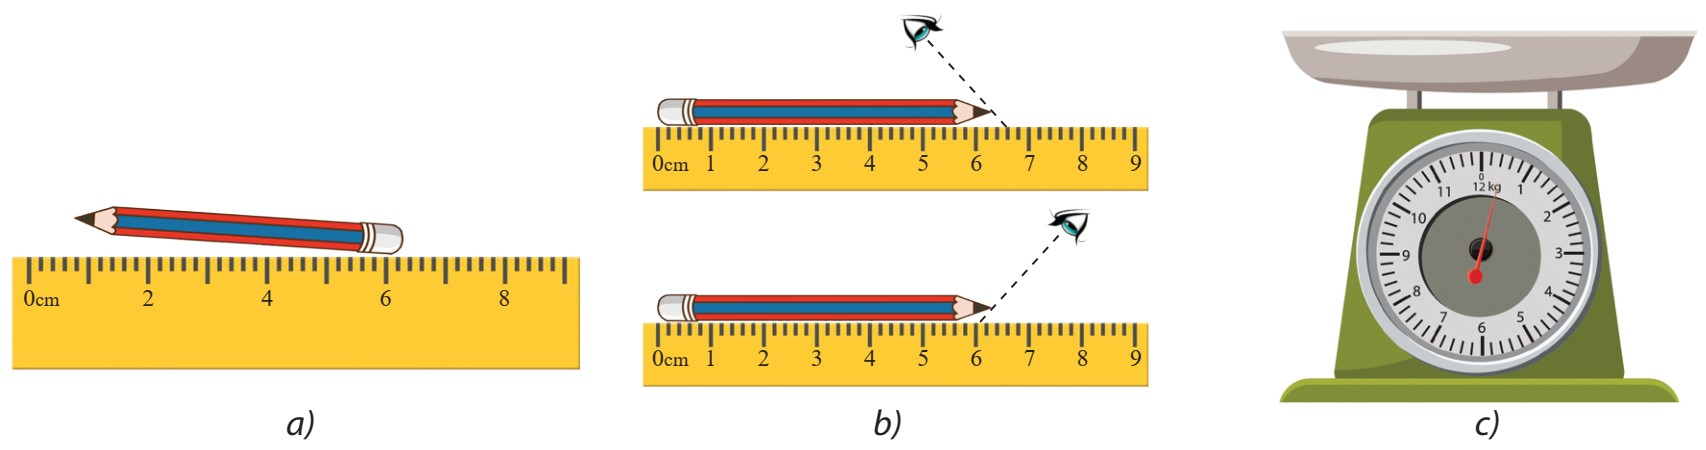
\includegraphics[width=0.7\linewidth]{figs/BAI3-1}
%\end{center}
%
%}\\
%\multicolumn{2}{|L{17cm}|}{\dotfill
%}\\
%\hline
%\end{longtable}
%\end{center}
%* Bài tập vận dụng 
%% ======================================================================
%\begin{ex}
%Bảng bên dưới thể hiện	kết quả đo khối lượng của một túi trái cây bằng cân đồng hồ. Em hãy xác định sai số tuyệt đối ứng với từng lần đo, sai số tuyệt đối và sai số tương đối của phép đo. Biết sai số dụng cụ là $\SI{0.1}{\kilogram}$.
%\begin{center}
%	\begin{longtable}{|M{5.5cm}|M{5.5cm}|M{5.5cm}|}
%		\hline
%		\thead{Lần đo} & $\xsi{m}{\left(\kilogram\right)}$ & $\xsi{\Delta m}{\left(\kilogram\right)}$\\
%		\hline
%		1 & 4,2 &\\
%		\hline
%		2 & 4,4 &\\
%		\hline
%		3 & 4,4 &\\
%		\hline
%		4 & 4,2 &\\
%		\hline
%		\thead{Trung bình}&$\overline{m}=$ &$\overline{\Delta m}=$\\
%		\hline
%	\end{longtable}
%\end{center}
%Sai số tuyệt đối của phép đo: $\Delta m=\overline{\Delta m}+\Delta m_{\text{dc}}=$ \dotfill\\
%Sai số tương đối của phép đo: $\delta m=\dfrac{\Delta m}{\overline{m}}\cdot\SI{100}{\percent}=$ \dotfill\\
%Kết quả phép đo: $m=\overline{m}\pm\Delta m=$ \dotfill
%	\loigiai{
%\begin{center}
%	\begin{longtable}{|M{5.5cm}|M{5.5cm}|M{5.5cm}|}
%		\hline
%		\thead{Lần đo} & $\xsi{m}{\left(\kilogram\right)}$ & $\xsi{\Delta m}{\left(\kilogram\right)}$\\
%		\hline
%		1 & 4,2 &0,1\\
%		\hline
%		2 & 4,4 &0,1\\
%		\hline
%		3 & 4,4 &0,1\\
%		\hline
%		4 & 4,2 &0,1\\
%		\hline
%		\thead{Trung bình}&$\overline{m}=4,3$ &$\overline{\Delta m}=0,1$\\
%		\hline
%	\end{longtable}
%\end{center}
%Sai số tuyệt đối của phép đo: $\Delta m=\overline{\Delta m}+\Delta m_{\text{dc}}=\SI{0.1}{\kilogram}+\SI{0.1}{\kilogram}=\SI{0.2}{\kilogram}$\\
%Sai số tương đối của phép đo: $\delta m=\dfrac{\Delta m}{\overline{m}}\cdot\SI{100}{\percent}=\dfrac{0,2}{4,3}\cdot\SI{100}{\percent}\approx\SI{4.7}{\percent}$ \\
%Kết quả phép đo: $m=\overline{m}\pm\Delta m=\xsi{4,3\pm0,2}{\kilogram}$.
%}
%\end{ex}
%% ======================================================================
%\begin{ex}
%Giả sử chiều dài của hai đoạn thẳng có giá trị đo được lần lượt là $a=\xsi{51\pm1}{\centi\meter}$ và $b=\xsi{49\pm1}{\centi\meter}$. Trong các đại lượng được tính theo các cách sau đây, đại lượng nào có sai số tương đối lớn nhất?
%\begin{enumerate}[label=\Alph*.]
%	\item $a+b$.
%	\item $a-b$.
%	\item $a\times b$.
%	\item $\dfrac{a}{b}$.
%	
%\end{enumerate}	
%	\loigiai{
%Sai số tương đối của từng trường hợp là:
%\begin{enumerate}[label=\Alph*.]
%	\item $\overline{c}=\overline{a}+\overline{b}=\SI{100}{\centi\meter}$; $\Delta c=\Delta a+\Delta b=\SI{2}{\centi\meter}$.\\
%	Do đó $\delta c=\dfrac{\Delta c}{\overline{c}}\cdot\SI{100}{\percent}=\SI{2}{\percent}$.
%	\item $\overline{c}=\overline{a}-\overline{b}=\SI{2}{\centi\meter}$; $\Delta c=\Delta a+\Delta b=\SI{2}{\centi\meter}$.\\
%	Do đó $\delta c=\dfrac{\Delta c}{\overline{c}}\cdot\SI{100}{\percent}=\SI{100}{\percent}$.
%	\item $\delta c=\left(\dfrac{\Delta a}{\overline{a}}+\dfrac{\Delta b}{\overline{b}}\right)\cdot\SI{100}{\percent}=\SI{4}{\percent}$.
%	\item $\delta c=\left(\dfrac{\Delta a}{\overline{a}}+\dfrac{\Delta b}{\overline{b}}\right)\cdot\SI{100}{\percent}=\SI{4}{\percent}$.
%\end{enumerate}	
%Vậy trường hợp có sai số tương đối lớn nhất là trường hợp B.
%}
%\end{ex}





%\chapter{Bài 4. Chuyển động thẳng}
\begin{center}
	\textit{(6 tiết)}
\end{center}
\section{MỤC TIÊU DẠY HỌC}
\begin{center}
	\begin{longtable}{|M{2.5cm}|L{12.5cm}|M{2cm}|}
		\hline
		\thead{Biểu hiện\\ năng lực} & \thead{Mục tiêu} & \thead{STT}\\
		\hline
		\multicolumn{3}{|c|}{\textbf{ Năng lực vật lí}}\\
		
		\hline
		1.1& Từ hình ảnh hoặc ví dụ thực tiễn, định nghĩa được độ dịch chuyển. & 1\\
		\hline
		1.3 & So sánh được quãng đường đi được và độ dịch chuyển. &2\\
		\hline
		1.2 & Lập luận để rút ra được công thức tính tốc độ trung bình, định nghĩa được tốc độ theo một phương. & 3\\
		\hline
		1.4 & Dựa vào định nghĩa tốc độ theo một phương và độ dịch chuyển, rút ra được công thức tính và định nghĩa được vận tốc. & 4\\
		\hline
		1.2 &  Dựa trên số liệu cho trước, vẽ được đồ thị độ dịch chuyển – thời gian trong chuyển động thẳng.& 5\\
		\hline
		1.2 & Tính được tốc độ từ độ dốc của đồ thị độ dịch chuyển – thời gian. & 6\\
		\hline
		\hline
		1.2 & Vận dụng được công thức tính tốc độ, vận tốc. & 7\\
		\hline
		\multicolumn{3}{|c|}{\textbf{Năng lực chung}}\\
		\hline
		TC - TH& Tích cực thực hiện các nhiệm vụ GV đặt ra cho các nhóm, tích cực suy luận để đưa ra câu trả lời trong quá trình GV định hướng nội dung học tập	&8 \\
		\hline
		GT - HT & Tích cực đóng góp ý kiến trong quá trình thảo luận, biết sử dụng ngôn ngữ kết hợp với các loại phương tiện phi ngôn ngữ đa dạng để trình bày các kết quả thảo luận nhóm & 10\\
		\hline
	\end{longtable}
\end{center}
\section{THIẾT BỊ DẠY HỌC VÀ HỌC LIỆU}
\begin{itemize}
	\item Tivi/máy chiếu;
	\item SGK;
	\item Phiếu học tập.
\end{itemize}
\section{TIẾN TRÌNH DẠY HỌC}
\subsection{TIẾN TRÌNH}\newpage
\begin{center}
	\begin{longtable}{|L{2.75cm}|C{1.25cm}|L{5cm}|L{3.5cm}|L{4cm}|}
		\hline
		\thead{Tiến trình} & \thead{Mục\\tiêu} & \thead{Nội dung dạy học \\trọng tâm} & \thead{PP,\\ KTDH} & \thead{Phương pháp \\đánh giá}\\
		\hline
	\textbf{Hoạt động 1:} Phân biệt khái niệm quãng đường và độ dịch chuyển	&1, 2  & Phân biệt khái niệm quãng đường và độ dịch chuyển  & PPDH: Đàm thoại& GV đánh giá dựa trên câu trả lời của HS.\newline
	PP đánh giá: quan sát, nghe. \\
		\hline
		\textbf{Hoạt động 2:} Tìm hiểu khái niệm tốc độ	& 3  & Khái niệm và công thức tính tốc độ trung bình, tốc độ tức thời  & PPDH:  Đàm thoại\newline KTDH: Động não& GV đánh giá dựa trên câu trả lời của HS.\newline
		PP đánh giá: quan sát, nghe. \\
		\hline
		\textbf{Hoạt động 3:} Tìm hiểu khái niệm vận tốc	& 4  & Khái niệm và công thức tính vận tốc trung bình, vận tốc tức thời  & PPDH:  Đàm thoại\newline KTDH: Động não& GV đánh giá dựa trên câu trả lời của HS.\newline
		PP đánh giá: quan sát, nghe. \\
		\hline
		\textbf{Hoạt động 4:} Tìm hiểu đồ thị độ dịch chuyển - thời gian	& 5, 6, 8, 10  & Vẽ đồ thị độ dịch chuyển - thời gian từ số liệu cho trước, cách xác định tốc độ tức thời từ đồ thị độ dịch chuyển - thời gian  & PPDH:  Dạy học hợp tác& GV đánh giá dựa trên câu trả lời của HS và kết quả thảo luận nhóm.\newline
		PP đánh giá: quan sát, nghe. \\
		\hline
		\textbf{Hoạt động 5:} Luyện tập	& 6, 7  & Luyện tập tính tốc độ trung bình, vận tốc trung bình trong chuyển động thẳng, từ số liệu cho trước vẽ được đồ thị độ dịch chuyển - thời gian, tính tốc độ tức thời và vận tốc tức thời từ đồ thị độ dịch chuyển - thời gian. & PPDH:  Đàm thoại& GV đánh giá dựa trên bài tập cá nhân của học sinh.\newline
		PP đánh giá: quan sát, nghe. \\
		\hline
	\end{longtable}
\end{center}
\subsection{CÁC HOẠT ĐỘNG HỌC}
% ==========================================================================================
\hoatdong
{
	Tìm hiểu đồ thị độ dịch chuyển - thời gian
}
{\begin{itemize}
		\item HS định nghĩa được độ dịch chuyển.
		\item  HS so sánh được quãng đường đi được và độ dịch chuyển.
	\end{itemize}
	
}
{
	Kết quả trả lời của HS cho các câu hỏi gợi mở của GV:\\
	\textbf{Câu trả lời dự kiến:} 
	\begin{itemize}
		\item Trường hợp nhân vật đi từ O đến B:
		\begin{itemize}
			\item quãng đường đi là $s=OB$;
			\item độ dịch chuyển là $d=OB$.
		\end{itemize}
		\item Trường hợp nhân vật đi từ O đến B rồi về A:
		\begin{itemize}
			\item quãng đường đi là $s=OB+AB$;
			\item độ dịch chuyển là $d=OA$.
		\end{itemize}
	\end{itemize}
}
{\textit{\underline{* GV chuyển giao nhiệm vụ học tập}}\\
	GV giới thiệu cho học sinh về khái niệm quãng đường và độ dịch chuyển.\\
	GV yêu cầu HS xác định độ dịch chuyển và quãng đường đi được của nhân vật trong ví dụ hình bên trong các trường hợp
	\begin{center}
		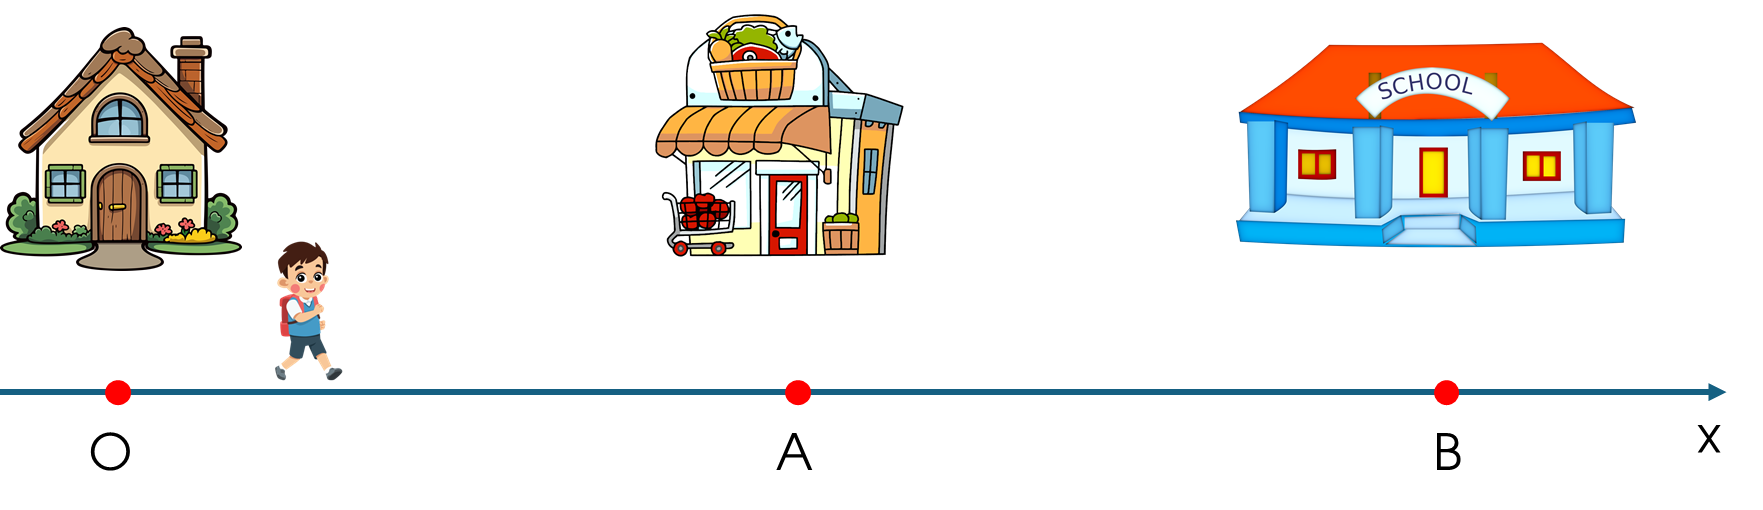
\includegraphics[width=0.9\linewidth]{figs/BAI4-1}
	\end{center}
	\begin{itemize}
		\item nhân vật đi từ nhà đến trường.
		\item nhân vật đi từ nhà đến trường rồi đến cửa hàng tạp hóa.
	\end{itemize}
	\textit{\underline{* HS thực hiện nhiệm vụ học tập}}\\
	HS tích cực trả lời câu hỏi gợi mở của GV.\\
	HS chú ý theo dõi, đặt câu hỏi.
}
% ==========================================================================================
\hoatdong
{
	Tìm hiểu khái niệm tốc độ
}
{\begin{itemize}
		\item HS nêu được tốc độ là đại lượng đặc trưng cho tính chất nhanh, chậm của chuyển động.
		\item HS lập luận rút ra được công thức tính tốc độ trung bình.
	\end{itemize}
	
}
{
	Kết quả trả lời của HS cho các câu hỏi gợi mở của GV:\\
	\textbf{Câu trả lời dự kiến:} Trung bình 1 giây vận động viên bơi được $\SI{2}{\meter}$ ở lần đầu và $\SI{1.79}{\meter}$ ở lần sau. Như vậy, lần đầu vận động viên này bơi nhanh hơn.
}
{\textit{\underline{* GV chuyển giao nhiệm vụ học tập}}\\
GV đặt ra tình huống để HS thảo luận theo nhóm đôi:\\
\textit{Một vận động viên bơi lội người Mỹ đã từng lập kỉ lục thế giới ở nội dung bơi bướm $\SI{100}{\meter}$ và $\SI{200}{\meter}$ với thời gian lần lượt là $\SI{49.82}{\second}$ và $\SI{111.51}{\second}$. Hãy lập luận để xác định vận động viên này bơi nhanh hơn trong trường hợp nào?}\\
Từ câu trả lời của HS, GV dẫn dắt đến khái niệm tốc độ trung bình.\\
GV giới thiệu cho HS khái niệm tốc độ tức thời.\\
GV đặt câu hỏi: \textit{Vậy số chỉ trên tốc kế là tốc độ trung bình hay tốc độ tức thời?}\\
\textit{\underline{* HS thực hiện nhiệm vụ học tập}}\\
HS tích cực trả lời câu hỏi gợi mở của GV.\\
HS chú ý theo dõi, đặt câu hỏi.\\
\textit{\underline{* HS báo cáo kết quả thực hiện nhiệm vụ học tập}}\\
GV lần lượt mời 1 HS trả lời câu hỏi và 1 HS khác nhận xét câu trả lời.\\
HS theo dõi, nhận xét, đặt câu hỏi.\\
GV chỉnh lí, hợp thức hoá kiến thức.
}
% ==========================================================================================
\hoatdong
{
	Tìm hiểu khái niệm vận tốc
}
{\begin{itemize}
		\item HS dựa vào định nghĩa tốc độ theo một phương và độ dịch chuyển, rút ra được công thức tính và định nghĩa được vận tốc.
		\item HS phân biệt được tốc độ trung bình và vận tốc trung bình.
	\end{itemize}

}
{
	Câu trả lời của HS cho câu hỏi gợi mở do GV đưa ra:\\
	\textbf{Câu trả lời dự kiến:} Cần phải biết thêm hướng chuyển động của hai người mới có thể xác định được vị trí gặp nhau.
}
{\textit{\underline{* GV chuyển giao nhiệm vụ học tập}}\\
	GV đặt câu hỏi gợi mở: \textit{Có hai người đi xe máy khởi hành cùng lúc từ thành phố A và thành phố B cách nhau $\SI{40}{\kilo\meter}$ với tốc độ không đổi $\SI{40}{\kilo\meter/\hour}$ và $\SI{60}{\kilo\meter/\hour}$ trên một đường thẳng. Em có thể xác định được thời điểm hai người gặp nhau không? Vì sao?}\\
	Từ câu trả lời của HS, GV rút ra kết luận: \textit{Tốc độ không cho biết hướng chuyển động. Trong các bài toán khảo sát vị trí của vật, ta cần quan tâm đến độ dịch chuyển của vật theo thời gian. Thay đại lượng $s$ trong công thức tốc độ trung bình bằng độ dịch chuyển $\vec{d}$ ta có được đại lượng mới, được gọi là vận tốc trung bình $\vec{v}_{\text{tb}}=\dfrac{\vec{d}}{\Delta t}=\dfrac{\Delta \vec{x}}{\Delta t}$.}\\
	GV đặt câu hỏi để đi đến phần lưu ý: \textit{Vậy khi nào thì tốc độ trung bình bằng với độ lớn của vận tốc trung bình?}\\
	GV giới thiệu khái niệm vận tốc tức thời.\\
	\textit{\underline{* HS thực hiện nhiệm vụ học tập}}\\
	HS tích cực trả lời câu hỏi gợi mở của GV.\\
	HS chú ý theo dõi, đặt câu hỏi.\\
	\textit{\underline{* HS báo cáo kết quả thực hiện nhiệm vụ học tập}}\\
	GV lần lượt mời 1 HS trả lời câu hỏi và 1 HS khác nhận xét câu trả lời.\\
	HS theo dõi, nhận xét, đặt câu hỏi.\\
	GV chỉnh lí, hợp thức hoá kiến thức.
}
% ==========================================================================================
\hoatdong
{
	Tìm hiểu đồ thị độ dịch chuyển - thời gian
}
{\begin{itemize}
		\item HS vẽ được đồ thị độ dịch chuyển - thời gian từ số liệu cho trước.
		\item HS xác định được tốc độ tức thời, vận tốc tức thời từ đồ thị độ dịch chuyển - thời gian.
	\end{itemize}
	
}
{
	Kết quả thảo luận nhóm của HS.
}
{\textit{\underline{* GV chuyển giao nhiệm vụ học tập}}\\
	GV ôn tập lại cho HS phần đồ thị hàm số bậc nhất, nội dung ôn tập như sau:
	\begin{itemize}
		\item Đồ thị hàm số $y=ax+b\ \left(a\neq0\right)$ là đường thẳng.
		\item Hệ số góc của đường thẳng $a=\tan\beta=\dfrac{\Delta y}{\Delta x}=\dfrac{y_{\mathrm{B}}-y_{\mathrm{A}}}{x_{\mathrm{B}}-x_{\mathrm{A}}}.$
	\end{itemize}
	\begin{center}
		\begin{tabular}{M{8cm}M{8cm}}
			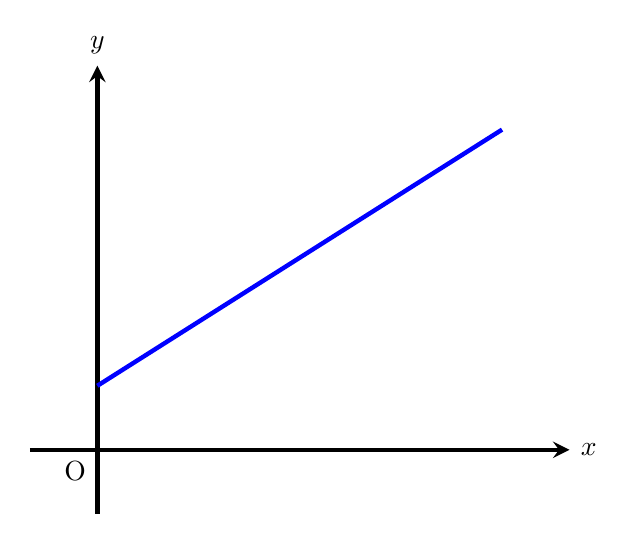
\begin{tikzpicture}  
				\begin{axis}[  ultra thick,
					xmin=-1,  
					xmax=7,  
					ymin=-1,  
					ymax=6, 
					samples=300,
				xtick=\empty,
				ytick=\empty,
					yticklabels=\empty,
					xticklabels=\empty,
					axis lines=center, 
					xlabel=$x$, 		ylabel=$y$,
					every axis y label/.style={at=(current axis.above origin),anchor=south},  
					every axis x label/.style={at=(current axis.right of origin),anchor=west},  ]
					\addplot [ultra thick, blue, smooth, domain=0:6] {1+2*x/3};
					\node[below left] at (axis cs: 0, 0) {O}; 
				\end{axis}  
			\end{tikzpicture} &
			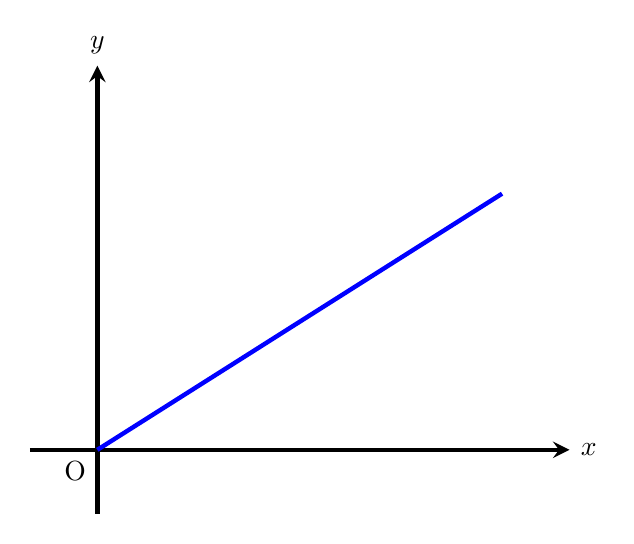
\begin{tikzpicture}  
				\begin{axis}[  ultra thick,
					xmin=-1,  
					xmax=7,  
					ymin=-1,  
					ymax=6, 
					xtick=\empty,
					ytick=\empty,
					samples=300,
					yticklabels=\empty,
					xticklabels=\empty,
					axis lines=center, 
					xlabel=$x$, 		ylabel=$y$,
					every axis y label/.style={at=(current axis.above origin),anchor=south},  
					every axis x label/.style={at=(current axis.right of origin),anchor=west},  ]
					\addplot [ultra thick, blue, smooth, domain=0:6] {2*x/3}; 
					\node[below left] at (axis cs: 0, 0) {O};
				\end{axis}  
			\end{tikzpicture}\\
			$b\neq 0$ & $b=0$
		\end{tabular}
	\end{center}
	\begin{center}
		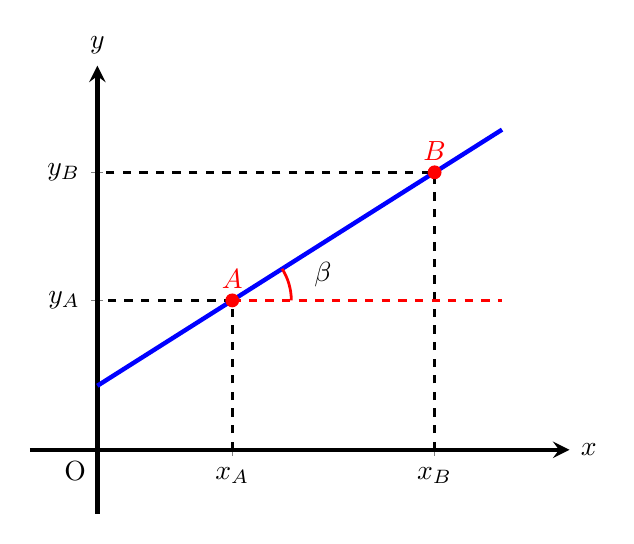
\begin{tikzpicture}  
			\begin{axis}[  ultra thick,
				xmin=-1,  
				xmax=7,  
				ymin=-1,  
				ymax=6, 
				samples=300,
				xtick={2, 5},
				ytick={2.3333, 4.3333},
				yticklabels={$y_A$, $y_B$},
				xticklabels={$x_A$, $x_B$},
				axis lines=center, 
				xlabel=$x$, 		ylabel=$y$,
				every axis y label/.style={at=(current axis.above origin),anchor=south},  
				every axis x label/.style={at=(current axis.right of origin),anchor=west},  ]
				\coordinate (A) at (axis cs: 2, 2.3333);
				\coordinate (B) at (axis cs: 5, 4.3333);
				\coordinate (C) at (axis cs: 6, 2.3333);
				\addplot [ultra thick, blue, smooth, domain=0:6] {1+2*x/3};
				\node[below left] at (axis cs: 0, 0) {O}; 
				\draw[dashed, line width=1pt] (axis cs: 2,0)--(A)--(axis cs:0,2.3333);
				\draw[dashed, line width=1pt] (axis cs: 5,0)--(B)--(axis cs:0,4.3333);
				\draw[dashed, line width=1pt, red] (A)--(axis cs:6,2.3333);
				\fill[red]   (A) circle[radius=2.5pt]  node [above] {$A$};
				\fill[red]   (B) circle[radius=2.5pt]  node [above] {$B$};
			\end{axis} 
			\tkzMarkAngle[size=0.75cm,color=red, line width=1pt](C,A,B);
			\tkzLabelAngle[color=black,pos=1.2](C,A,B){$\beta$}; 
		\end{tikzpicture}
		
	\end{center}
	\begin{itemize}
		\item Hệ số góc $a$ càng lớn thì góc $\beta$ càng lớn (đồ thị càng dốc).
	\end{itemize}
GV hướng dẫn HS xây dựng phương trình tọa độ của vật chuyển động thẳng đều:
\begin{itemize}
	\item Chất điểm chuyển động thẳng đều: 
	$$v=\dfrac{d}{\Delta t}=const\Rightarrow d=v\Delta t=v\left(t-t_0\right).$$
	\item Nếu chọn gốc thời gian lúc vật qua gốc toạ độ $(t_0=0)$, thì phương trình độ dịch chuyển của chất điểm so với gốc toạ độ: $d=v\cdot t$.\\
	Như vậy, đồ thị độ dịch chuyển thời gian của vật chuyển động thẳng đều là 1 đường thẳng:
	\begin{center}
		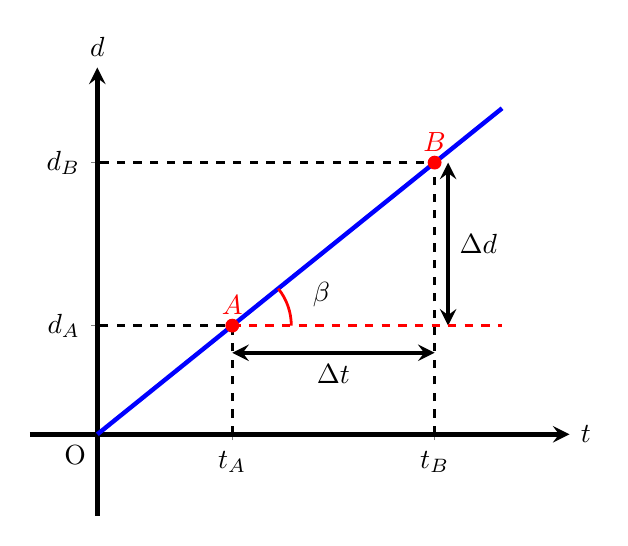
\begin{tikzpicture}  
			\begin{axis}[  ultra thick,
				xmin=-1,  
				xmax=7,  
				ymin=-1,  
				ymax=4.5, 
				samples=300,
				xtick={2, 5},
				ytick={1.3333, 3.3333},
				yticklabels={$d_A$, $d_B$},
				xticklabels={$t_A$, $t_B$},
				axis lines=center, 
				xlabel=$t$, 		ylabel=$d$,
				every axis y label/.style={at=(current axis.above origin),anchor=south},  
				every axis x label/.style={at=(current axis.right of origin),anchor=west},  ]
				\coordinate (A) at (axis cs: 2, 1.3333);
				\coordinate (B) at (axis cs: 5, 3.3333);
				\coordinate (C) at (axis cs: 6, 1.3333);
				\draw[stealth-stealth] (axis cs: 2,1)--(axis cs: 5,1);
				\draw[stealth-stealth] (axis cs: 5.2,3.3333)--(axis cs: 5.2,1.3333);
				\addplot [ultra thick, blue, smooth, domain=0:6] {2*x/3};
				\node[below left] at (axis cs: 0, 0) {O}; 
				\draw[dashed, line width=1pt] (axis cs: 2,0)--(A)--(axis cs:0,1.3333);
				\draw[dashed, line width=1pt] (axis cs: 5,0)--(B)--(axis cs:0,3.3333);
				\draw[dashed, line width=1pt, red] (A)--(axis cs:6,1.3333);
				\fill[red]   (A) circle[radius=2.5pt]  node [above] {$A$};
				\fill[red]   (B) circle[radius=2.5pt]  node [above] {$B$};
				\node[below] at (axis cs: 3.5, 1) {$\Delta t$};
				\node[right] at (axis cs: 5.2, 2.3333) {$\Delta d$};
			\end{axis} 
			\tkzMarkAngle[size=0.75cm,color=red, line width=1pt](C,A,B);
			\tkzLabelAngle[color=black,pos=1.2](C,A,B){$\beta$}; 
		\end{tikzpicture}
		
	\end{center}
	\begin{itemize}
		\item Độ dốc của đồ thị $d\left(t\right)$ càng lớn, vật chuyển động càng nhanh (tốc độ càng lớn): $v=\tan\beta=\dfrac{\Delta d}{\Delta t}=\dfrac{d_{\mathrm{B}}-d_{\mathrm{A}}}{t_{\mathrm{B}}-t_{\mathrm{A}}}$.
		\item Nếu hệ số góc của đồ thị $d\left(t\right)$ âm, vật đang chuyển động ngược chiều dương.
	\end{itemize}
\end{itemize}
GV yêu cầu HS thảo luận nhóm đôi để thực hiện ví dụ 1 trong thời gian 15 phút, sau 15 phút GV mời đại diện của 1 nhóm HS bất kì lên bảng giải bài.\\
GV dẫn dắt HS từ phương trình độ dịch chuyển - thời gian của vật chuyển động thẳng đều suy ra phương trình tọa độ - thời gian của vật chuyển động thẳng đều:
 $$d=x-x_0=vt\Rightarrow x=x_0+vt.$$
 GV dùng kĩ thuật tia chớp, yêu cầu HS thực hiện ví dụ 2, HS có kết quả nhanh nhất sẽ lên bảng giải bài và nhận được 1 điểm cộng.\\
 GV yêu cầu HS thảo luận nhóm đôi để thực hiện ví dụ 3. Sau 15 phút, GV mời đại diện 1 nhóm HS lên bảng trình bày kết quả. \\
 \textit{\underline{* HS thực hiện nhiệm vụ học tập}}\\
 HS theo dõi, tích cực trả lời câu hỏi của GV.\\
 HS thảo luận nhóm đôi để thực hiện ví dụ 1 và ví dụ 3.\\
 HS làm việc cá nhân để thực hiện ví dụ 2.\\
 \textit{\underline{* HS báo cáo kết quả thực hiện nhiệm vụ học tập}}\\
 HS lên bảng trình bày kết quả ví dụ 1, ví dụ 2, ví dụ 3.\\
 Các nhóm HS theo dõi bài làm của nhóm bạn để đặt câu hỏi, nhận xét.\\
 GV chỉnh lí, hợp thức hóa kiến thức.
 
}
%%%%%%%%%%%%%%%%%%%%%%%%%%%%%%%%%%%%%%%%%%%%%
\hoatdong{
	Luyện tập.
}
{
\begin{itemize}
	\item HS tính được tốc độ từ độ dốc của đồ thị độ dịch chuyển - thời gian.
	\item HS vận dụng được công thức tính tốc độ, vận tốc.
\end{itemize}
}
{
	Bài tập cá nhân của học sinh.
}
{
	\textit{\underline{GV chuyển giao nhiệm vụ học tập}}\\
	GV lần lượt chuyển giao từng bài tập, yêu cầu HS hoạt động cá nhân để giải.\\
	\textit{\underline{HS thực hiện nhiệm vụ học tập}}\\
	HS \textit{(làm việc cá nhân)}:  Giải bài tập trong phiếu bài tập được GV giao. 
	
	GV: Theo dõi để phát hiện các HS gặp khó khăn, từ đó đưa ra sự định hướng, hỗ trợ phù hợp cho mỗi HS.\\
	\textit{\underline{HS báo cáo kết quả thực hiện nhiệm vụ học tập}}\\
	GV: Mời HS lên bảng giải bài tập.
	
	HS: Đặt câu hỏi, góp ý.
	
	GV: Chỉnh lí, hợp thức hoá kiến thức.
}
\section{HỒ SƠ DẠY HỌC}
\subsection{NỘI DUNG DẠY HỌC}
\begin{enumerate}[label=\bfseries\Roman*.]
\item \textbf{Tốc độ trung bình}\\ Tốc độ trung bình của vật được xác định bằng thương số giữa quãng đường vật đi được và thời gian để vật thực hiện được quãng đường ấy.
$$\overline{v_{\mathrm{tb}}}=\dfrac{S}{\Delta t}=\dfrac{S_1+S_2+\dots+S_n}{\Delta t_1+\Delta t_2+\dots+\Delta t_n}.$$
Trong đó:
\begin{itemize}
	\item $\overline{v_{\mathrm{tb}}}$: Tốc độ trung bình có đơn vị trong hệ SI là $\si{\meter/\second}$;
	\item $S$: quãng đường vật đi được luôn dương và có đơn vị trong hệ SI là $\si{\meter}$;
	\item $\Delta t$: thời gian có đơn vị trong hệ SI là $\si{\second}$.
\end{itemize}	
	\item \textbf{Độ dịch chuyển}\\ Độ dịch chuyển là một đại lượng vector $\vec{d}$ có gốc tại vị trí ban đầu, hướng từ vị trí đầu đến vị trí cuối, độ lớn bằng khoảng cách giữa vị trí đầu và vị trí cuối. Độ dịch chuyển có thể nhận giá trị dương, âm hoặc bằng không.
	$$d=\Delta x=x_2-x_1.$$
	Trong đó:
	\begin{itemize}
		\item $x_1$: tọa độ lúc ban đầu của vật;
		\item $x_2$: tọa độ cuối của vật.
	\end{itemize}
	\textbf{* Chú ý:} Độ dịch chuyển $d$ trùng với quãng đường $s$ khi vật chỉ chuyển động theo một chiều và chọn chiều đó làm chiều dương của trục tọa độ.
	\item \textbf{Vận tốc trung bình}
	$$v_{\mathrm{tb}}=\dfrac{d}{\Delta t}=\dfrac{\Delta x}{\Delta t}=\dfrac{x_2-x_1}{t_2-t_1}.$$
	\item \textbf{Phương trình chuyển động thẳng đều}
	$$x=x_0+v\left(t-t_0\right)$$
	Trong đó:
	\begin{itemize}
		\item $x$ là tọa độ của vật ở thời điểm $t$;
		\item $x_0$ là tọa độ của vật ở thời điểm ban đầu $t_0$;
		\item $v$ là vận tốc tức thời.
	\end{itemize}
	\item \textbf{Đồ thị độ dịch chuyển - thời gian}\\
	Ta xét chất điểm chuyển động thẳng đều:
	\begin{itemize}
		\item Chuyển động thẳng đều là chuyển động thẳng, trong đó chất điểm có vận tốc tức thời không đổi.
		\item Gọi $x_0$ là tọa độ của chất điểm tại thời điểm ban đầu $t_0$, $x$ là tọa độ thời điểm $t$ sau đó và độ dịch chuyển $d=x-x_0$. Vận tốc của chất điểm bằng: $v=\dfrac{d}{t}=\dfrac{x-x_0}{t}=\text{hằng số}$.\\
	\end{itemize}
	Từ đó: $d=vt\hspace{0.5cm} (1)$ và $x=x_0+vt\hspace{0.5cm}(2)$.\\
	Ta biểu diễn phương trình (1) và (2) bằng đồ thị.\\
	* Đồ thị $\left(d-t\right)$ là một đường thẳng đi qua gốc tọa độ. Một số dạng đồ thị sau:
	\begin{center}
		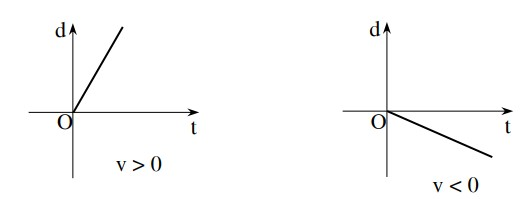
\includegraphics[scale=0.9]{../figs/G10-BAI4-1}
	\end{center}
	* Đồ thị $\left(x-t\right)$ là một đường xiên góc xuất phát từ điểm $\left(x_0;0\right)$. Một số dạng đồ thị sau:
	\begin{center}
		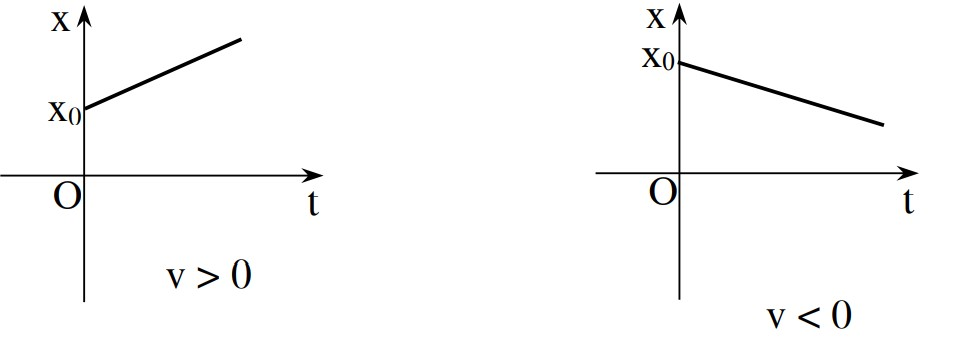
\includegraphics[scale=0.5]{../figs/G10-BAI4-2}
	\end{center}
\end{enumerate}
\subsection{CÁC HỒ SƠ KHÁC}
\textbf{* Các câu hỏi ví dụ}\\
\setcounter{ex}{0}
% ======================================================================
\begin{ex}
	Một chiếc xe đồ chơi đang chuyển động đều trên các đoạn thẳng có độ dịch chuyển tại các thời điểm khác nhau được cho trong bảng dưới đây
	\begin{center}
		\begin{tabular}{|M{3cm}|M{1cm}|M{1cm}|M{1cm}|M{1cm}|M{1cm}|M{1cm}|M{1cm}|M{1cm}|M{1cm}|M{1cm}|M{1cm}|}
			\hline
			\textbf{Thời gian} & 0 & 2 & 4 & 6 & 8 & 10 & 12 & 14 & 16 & 18 & 20\\
			\hline
			\textbf{Độ dịch chuyển $\left(\si{\meter}\right)$} & 0 & 3 & 4 & 4 & 4 & 7 & 10 & 8 & 6 & 4 & 4\\
			\hline
		\end{tabular}
	\end{center}
	\begin{enumerate}[label=\alph*)]
		\item Hãy vẽ đồ thị độ dịch chuyển – thời gian của xe đồ chơi.
		\item Hãy xác định vận tốc và tốc độ tức thời tại các thời điểm $\SI{2}{\second}$, $\SI{6}{\second}$, $\SI{10}{\second}$ và $\SI{16}{\second}$.
		\end{enumerate}
	\loigiai{
	\begin{enumerate}[label=\alph*)]
		\item Đồ thị độ dịch chuyển – thời gian của xe đồ chơi
		\begin{center}
			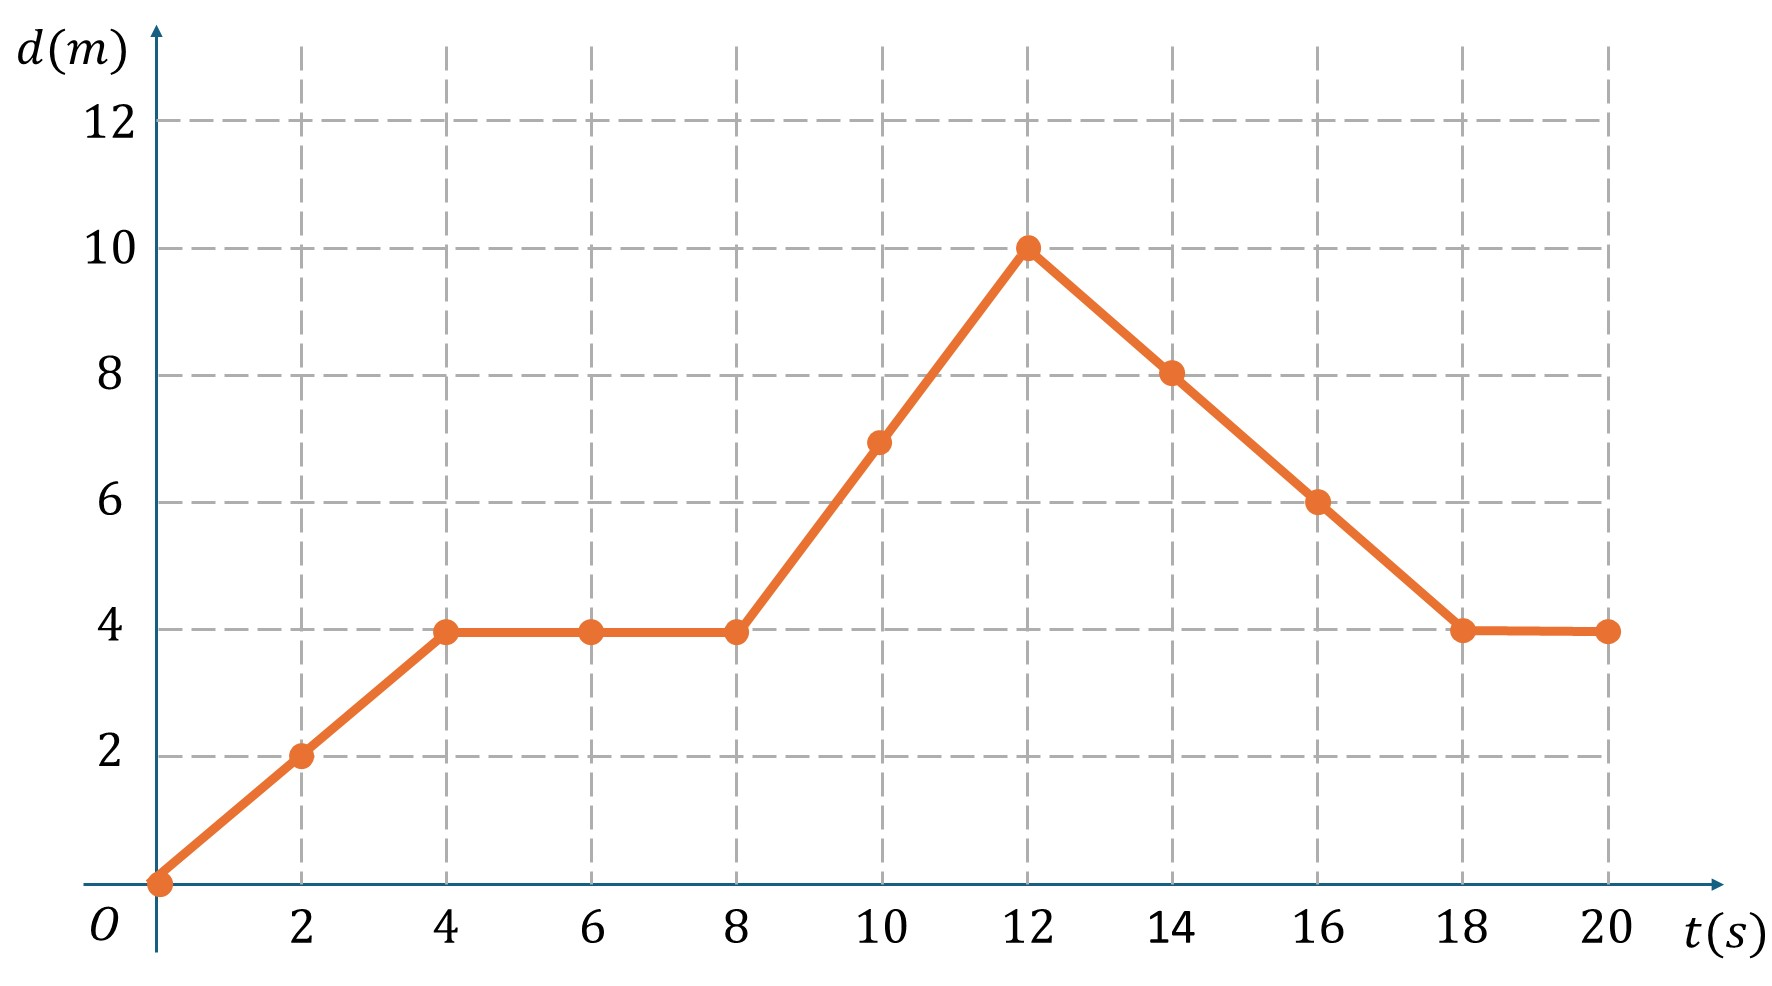
\includegraphics[scale=0.4]{../figs/G10-BAI4-3}
		\end{center}
		\item Vận tốc tức thời và tốc độ tức thời tại các thời điểm:
		\begin{itemize}
			\item $t=\SI{2}{\second}$:\\
			$v=\dfrac{2-0}{2-0}=\SI{1}{\meter/\second}$; $\left|v\right|=\SI{1}{\meter/\second}$.
			\item $t=\SI{6}{\second}$:\\
			$v=\dfrac{4-4}{6-4}=\SI{0}{\meter/\second}$; $\left|v\right|=\SI{0}{\meter/\second}$.
			\item $t=\SI{10}{\second}$:\\
			$v=\dfrac{10-4}{12-8}=\SI{1.5}{\meter/\second}$; $\left|v\right|=\SI{1.5}{\meter/\second}$.
			\item $t=\SI{16}{\second}$:\\
			$v=\dfrac{4-10}{18-12}=\SI{-1}{\meter/\second}$; $\left|v\right|=\SI{1}{\meter/\second}$.
		\end{itemize}
	\end{enumerate}
	}
\end{ex}
% ======================================================================
\begin{ex}
	Phương trình chuyển động của chất điểm dọc theo trục Ox có dạng $x=135-45t$ ($x$ đo bằng kilomet, $t$ đo bằng giờ).
	\begin{enumerate}[label=\alph*)]
		\item Chất điểm xuất phát từ điểm nào? Xác định trạng thái chuyển động của chất điểm.
		\item Xác định vị trí chất điểm tại thời điểm $t=\SI{2}{\hour}$.
		\item Xác định thời điểm chất điểm qua gốc tọa độ.
	\end{enumerate}
	\loigiai{
	\begin{enumerate}[label=\alph*)]
		\item  Chất điểm xuất phát từ điểm có tọa độ $x_0=\SI{135}{\kilo\meter}$ và chuyển động thẳng đều.
		\item Tại thời điểm $t=\SI{2}{\hour}$ thì $x=\SI{45}{\kilo\meter}$.
		\item Chất điểm qua gốc tọa độ thì $x=0\Rightarrow t=\SI{3}{\hour}$.
	\end{enumerate}
	}
\end{ex}
% ======================================================================
\begin{ex}
	Lúc 6 giờ sáng một người đi xe đạp đuổi theo một người đi bộ đã đi được $\SI{8}{\kilo\meter}$. Cả hai chuyển động thẳng đều với các tốc độ lần lượt là $\SI{12}{\kilo\meter/\hour}$ và $\SI{4}{\kilo\meter/\hour}$.
	\begin{enumerate}[label=\alph*)]
		\item Lập phương trình chuyển động của mỗi người trong cùng hệ quy chiếu.
		\item Vẽ đồ thị tọa độ - thời gian của hai người trên cùng hệ trục tọa độ.
		\item Xác định thời điểm và vị trí hai người gặp nhau.
		
	\end{enumerate}
	\loigiai{
	\begin{enumerate}[label=\alph*)]
		\item Chọn gốc tọa độ tại vị trí xuất phát của người đi xe đạp, chiều dương cùng chiều chuyển động của hai người. Gốc thời gian lúc 6 giờ sáng.\\
		Phương trình chuyển động của mỗi người:
		$$\begin{cases}
			x_{\text{xđ}}=12t\\
			x_{\text{b}}=8+4t
		\end{cases}\left(\si{\kilo\meter}; \si{\hour}\right).$$
		\item Vẽ đồ thị tọa độ - thời gian của hai người trên cùng hệ trục tọa độ
		\begin{center}
			\begin{tikzpicture}  
				\begin{axis}[  ultra thick,
					xmin=0,  
					xmax=2.25,  
					xtick={0,0.5,...,2},
					ytick={0,12,24},
					minor x tick num=0,
					minor y tick num=0,
					ymin=0,  
					ymax=28, 
					samples=300,
					axis lines=center, 
					grid style={step=1, line width =0.4pt, color=gray!40!white},
					grid=both, %giới hạn ô lưới
					major grid style={line width=0.8pt,gray!75!white},
					xlabel=$\xsi{t}{\left(\si{\hour}\right)}$, 		ylabel=$\xsi{x}{\left(\si{\kilo\meter}\right)}$,
					every axis y label/.style={at=(current axis.above origin),anchor=south},  
					every axis x label/.style={at=(current axis.right of origin),anchor=west},  ]
					\addplot [line width=1.5pt, red, smooth, domain=0:2] {12*x} node[right] {$x_{\text{xđ}}$}; 
					\addplot [line width=1.5pt, blue, smooth, domain=0:2] {8+4*x} node[right] {$x_{\text{b}}$}; 
					\coordinate (O) at (axis cs: 0,0);
				\end{axis}  
				\node[below left] at (O) {0};
			\end{tikzpicture}
		\end{center}
		\item Dựa vào đồ thị, hai người gặp nhau lúc $t=\SI{1}{\hour}$ tại vị trí cách gốc tọa độ $x=\SI{12}{\kilo\meter}$.
	\end{enumerate}
	}
\end{ex}
\subsection{Bài tập}
\setcounter{ex}{0}
\textbf{BÀI TẬP TRẮC NGHIỆM}
% ===================================================================
\begin{ex}
	Một chiếc xe ô tô xuất phát từ A lúc 6 giờ sáng, chuyển động thẳng đều tới B, cách A $\SI{180}{\kilo\meter}$. Xe tới B lúc 8 giờ 30 phút. Sau 30 phút đỗ tại B, xe chạy ngược về A với tốc độ $\SI{60}{\kilo\meter/\hour}$. Ô tô về tới A lúc
	\choice
	{$\SI{10}{\hour}$}
	{\True $\SI{12}{\hour}$}
	{$\SI{11}{\hour}$}
	{$\SI{10.5}{\hour}$}
	\loigiai{}
\end{ex}
% ===================================================================
\begin{ex}
	Một xe chuyển động thẳng không đổi chiều có tốc độ trung bình là $\SI{20}{\kilo\meter/\hour}$ trên  $\frac{1}{4}$ đoạn đường đầu và $\SI{40}{\kilo\meter/\hour}$ trên $\frac{3}{4}$ đoạn đường còn lại. Tốc độ trung bình của xe trên cả đoạn đường là 	
	\choice
	{$\SI{30}{\kilo\meter/\hour}$}
	{\True $\SI{32}{\kilo\meter/\hour}$}
	{$\SI{26.67}{\kilo\meter/\hour}$}
	{$\SI{35}{\kilo\meter/\hour}$}
	\loigiai{}
\end{ex}
% ===================================================================
\begin{ex}
	Một chất điểm chuyển động dọc theo trục $Ox$ có phương trình tọa độ $x=4-10t$ trong đó $x$ tính theo đơn vị $\si{\kilo\meter}$ và $t$ tính theo đơn vị giờ. Quãng đường đi được của chất điểm sau 2 giờ chuyển động là
	\choice
	{$\SI{8}{\kilo\meter}$}
	{$\SI{16}{\kilo\meter}$}
	{\True $\SI{20}{\kilo\meter}$}
	{$\SI{12}{\kilo\meter}$}
	\loigiai{}
\end{ex}
% ===================================================================
\begin{ex}
	Cho đồ thị tọa độ - thời gian của một chiếc xe chuyển động thẳng như hình bên dưới. 
	\begin{center}
		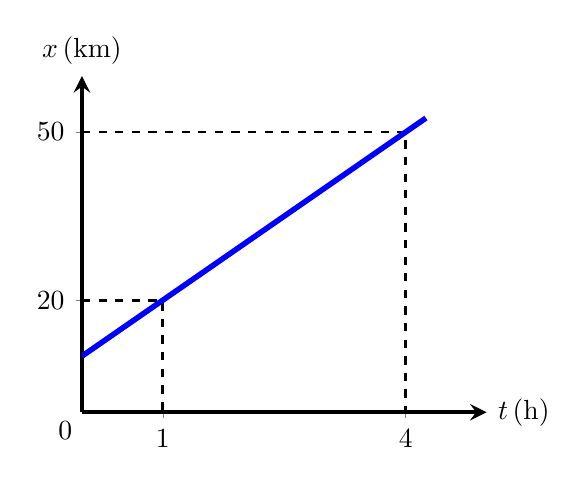
\begin{tikzpicture}  
			\begin{axis}[  ultra thick,scale=0.75,
				xmin=0,  
				xmax=5,  
				xtick={0,1,4},
				ytick={0,20,50},
				minor x tick num=0,
				minor y tick num=0,
				ymin=0,  
				ymax=60, 
				samples=300,
				axis lines=center, 
				xlabel=$\xsi{t}{\left(\si{\hour}\right)}$, 		ylabel=$\xsi{x}{\left(\si{\kilo\meter}\right)}$,
				every axis y label/.style={at=(current axis.above origin),anchor=south},  
				every axis x label/.style={at=(current axis.right of origin),anchor=west},  ]
				\draw[dashed, line width=1pt] (axis cs: 0,20)--(axis cs:1,20)--(axis cs:1,0);
				\draw[dashed, line width=1pt] (axis cs:0,50)--(axis cs:4,50)--(axis cs:4,0);
				\addplot [line width=2pt, blue, smooth, domain=0:4.25] {20+10*(x-1)};  
				\coordinate (O) at (axis cs: 0,0);
			\end{axis}  
			\node[below left] at (O) {0};
		\end{tikzpicture}
	\end{center}
	Phương trình tọa độ của xe là
	
	\choice
	{$x=15+5t$}
	{\True $x=10+10t$}
	{$x=20+10t$}
	{$x=-10+15t$}
	\loigiai{}
\end{ex}
% ===================================================================
\begin{ex}
	Đồ thị độ dịch chuyển – thời gian của một vật chuyển động như hình vẽ. Vật chuyển động
	\begin{center}
		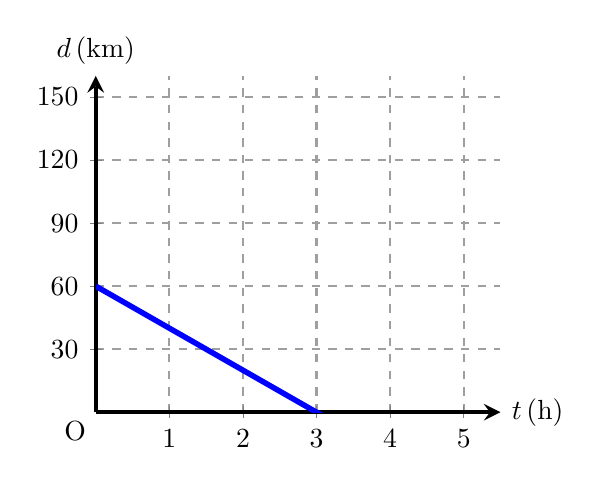
\begin{tikzpicture}  
			\begin{axis}[  ultra thick, scale=0.75,
				xmin=0,  
				xmax=5.5,  
				xtick={0,1,...,5},
				ytick={0,30,...,150},
				minor x tick num=0,
				minor y tick num=0,
				ymin=0,  
				ymax=160, 
				samples=300,
				axis lines=center, 
				grid style={step=1, line width =0.4pt, color=gray!40!white},
				grid=both, %giới hạn ô lưới
				major grid style={line width=0.8pt,gray!75!white, dashed},
				xlabel=$\xsi{t}{\left(\si{\hour}\right)}$, 		ylabel=$\xsi{d}{\left(\si{\kilo\meter}\right)}$,
				every axis y label/.style={at=(current axis.above origin),anchor=south},  
				every axis x label/.style={at=(current axis.right of origin),anchor=west},  ]
				\addplot [line width=2pt, blue, smooth, domain=0:5] {60-20*x};  
				\coordinate (O) at (axis cs: 0,0);
			\end{axis}  
			\node[below left] at (O) {O};
		\end{tikzpicture}
	\end{center}
	\choice
	{cùng chiều dương với tốc độ $\SI{60}{\kilo\meter/\hour}$}
	{\True ngược chiều dương với tốc độ $\SI{20}{\kilo\meter/\hour}$}
	{cùng chiều dương với tốc độ $\SI{20}{\kilo\meter/\hour}$}
	{ngược chiều dương với tốc độ $\SI{60}{\kilo\meter/\hour}$}
	\loigiai{}
\end{ex}
% ===================================================================
\begin{ex}
	Kết luận nào sau đây là \textbf{đúng} khi nói về độ dịch chuyển và quãng đường đi được của một vật?	
	\choice
	{Độ dịch chuyển và quãng đường đi được đều là đại lượng vô hướng}
	{\True Độ dịch chuyển là đại lượng vector còn quãng đường đi được là đại lượng vô hướng}
	{Độ dịch chuyển và quãng đường đi được đều là đại lượng vector}
	{Độ dịch chuyển và quãng đường đi được đều là đại lượng không âm}
	\loigiai{}
\end{ex}
% ===================================================================
\begin{ex}
	Khi vật chuyển động thẳng đều cùng chiều dương thì đồ thị $d - t$ của vật có dạng là
	\choice
	{đường thẳng vuông góc với trục $Od$}
	{\True đường thẳng xiên góc đi lên}
	{đường thẳng xiên góc đi xuống}
	{đường thẳng vuông góc với trục $Ot$}
	\loigiai{}
\end{ex}
%% ===================================================================
%\begin{ex}
%	Cho đồ thị độ dịch chuyển – thời gian của một vật như hình. Chọn phát biểu \textbf{đúng}.	
%	\begin{center}
%		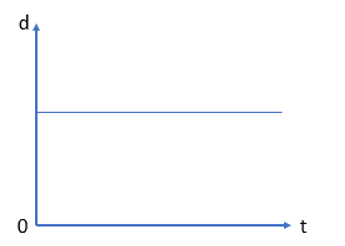
\includegraphics[width=0.25\linewidth]{figs/VN10-2023-PH-TP005-P-1}
%	\end{center}
%	\choice
%	{Vật đang chuyển động thẳng đều theo chiều dương}
%	{Vật đang chuyển động thẳng đều theo chiều âm}
%	{\True Vật đang đứng yên}
%	{Vật chuyển động thẳng đều theo chiều dương rồi đổi chiều chuyển động ngược lại}
%	\loigiai{}
%\end{ex}

% ===================================================================
\begin{ex}
	Một vật bắt đầu chuyển động từ điểm O đến điểm A, sau đó chuyển động về điểm B. Quãng đường và độ dịch chuyển của vật tương ứng là	
	\begin{center}
		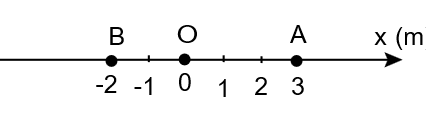
\includegraphics[width=0.4\linewidth]{figs/VN10-2022-PH-TP004-P-2}
	\end{center}
	\choice
	{$\SI{2}{\meter}$; $\SI{-2}{\meter}$}
	{\True $\SI{8}{\meter}$; $\SI{-2}{\meter}$}
	{$\SI{2}{\meter}$; $\SI{2}{\meter}$}
	{$\SI{8}{\meter}$; $\SI{-8}{\meter}$}
	\loigiai{}
\end{ex}
% ===================================================================
\begin{ex}
	“Lúc 15 giờ 30 phút hôm qua, xe chúng tôi đang chạy trên quốc lộ 5, cách Hải Dương 10 km”. Việc xác định vị trí của ô tô như trên còn thiếu yếu tố gì?	
	\choice
	{Vật làm mốc}
	{\True Chiều dương trên đường đi}
	{Mốc thời gian}
	{Thước đo và đồng hồ}
	\loigiai{}
\end{ex}

% ===================================================================
\begin{ex}
	
	Hai người đi xe đạp từ A đến C, người thứ nhất đi theo đường từ A đến B, rồi từ B đến C; người thứ hai đi thẳng từ A đến C. Cả hai đều về đích cùng một lúc.\\
	Hãy chọn kết luận \textbf{sai}.	
	\immini{
		\choice
		{Người thứ nhất đi được quãng đường $\SI{8}{\kilo\meter}$}
		{Độ dịch chuyển của người thứ nhất và người thứ hai bằng nhau}
		{\True Độ dịch chuyển và quãng đường đi được của người thứ nhất bằng nhau}
		{Độ dịch chuyển của người thứ nhất là $\SI{5.7}{\kilo\meter}$, hướng $\SI{45}{\degree}$ Đông – Bắc}
	}
	{
		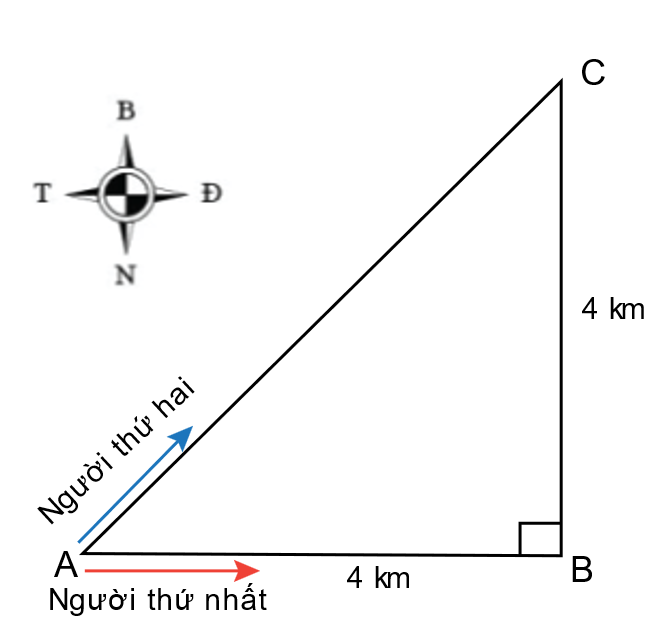
\includegraphics[width=0.5\linewidth]{figs/VN10-2022-PH-TP004-P-3}
	}
	\loigiai{}
	
\end{ex}
% ===================================================================
\begin{ex}
	Khi nhìn vào tốc kế của ô tô đang chạy, số chỉ trên tốc kế cho ta biết
	\choice
	{gia tốc tức thời của ô tô}
	{vận tốc tức thời của ô tô}
	{\True tốc độ tức thời của ô tô}
	{tốc độ trung bình của ô tô}
	\loigiai{}
\end{ex}
% ===================================================================
\begin{ex}
	Một máy bay phản lực có tốc độ $\SI{700}{\kilo\meter/\hour}$. Nếu muốn bay liên tục trên khoảng cách $\SI{1400}{\kilo\meter}$ thì máy bay phải bay trong thời gian là
	\choice
	{\True $\SI{2}{\hour}$}
	{$\SI{3}{\hour}$}
	{$\SI{2}{\hour}\SI{30}{\minute}$}
	{$\SI{1}{\hour}\SI{30}{\minute}$}
	\loigiai{Thời gian máy bay bay quãng đường $\SI{1400}{\kilo\meter}$:
		$$t=\dfrac{s}{v}=\SI{2}{\hour}.$$}
\end{ex}
% ===================================================================
\begin{ex}
	Đồ thị độ dịch chuyển – thời gian trong chuyển động thẳng của một chất điểm có dạng như hình vẽ.\\
	Trong thời gian nào xe chuyển động thẳng đều?
	\begin{center}
		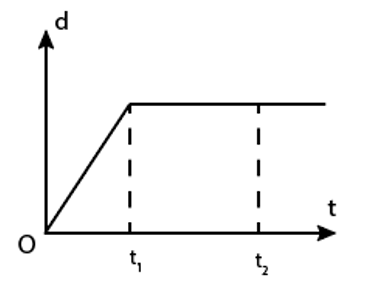
\includegraphics[width=0.25\linewidth]{figs/VN10-2023-PH-TP005-P-4}
	\end{center}
	\choice
	{\True Trong khoảng thời gian từ $0$ đến $t_1$}
	{Trong khoảng thời gian từ $0$ đến $t_2$}
	{Trong khoảng thời gian từ $t_1$ đến $t_2$}
	{Không có lúc nào xe chuyển động thẳng đều}
	\loigiai{}
\end{ex}
% ===================================================================
\begin{ex}
	Phương trình chuyển động của một chất điểm dọc theo trục $Ox$ có dạng: $x = 5 + 60t$ ($x$ đo bằng kilomét và $t$ đo bằng giờ). Chất điểm đó xuất phát từ điểm nào và chuyển động với vận tốc bằng bao nhiêu?
	\choice
	{Từ điểm $O$, với vận tốc $\SI{5}{\kilo\meter/\hour}$}
	{Từ điểm $O$, với vận tốc $\SI{60}{\kilo\meter/\hour}$}
	{Từ điểm cách $O$ $\SI{5}{\kilo\meter/\hour}$, với vận tốc $\SI{5}{\kilo\meter/\hour}$}
	{\True Từ điểm cách $O$ $\SI{5}{\kilo\meter/\hour}$, với vận tốc $\SI{60}{\kilo\meter/\hour}$}
	\loigiai{}
\end{ex}
% ===================================================================
\begin{ex}
	Phương trình chuyển động của một chất điểm dọc theo $Ox$ có dạng: $x=5t-12$ (km), với $t$ đo bằng giờ. Độ dịch chuyển của chất điểm từ $\SI{2}{\hour}$ đến $\SI{4}{\hour}$ là	
	\choice
	{$\SI{8}{\kilo\meter}$}
	{$\SI{6}{\kilo\meter}$}
	{\True $\SI{10}{\kilo\meter}$}
	{$\SI{2}{\kilo\meter}$}
	\loigiai{}
\end{ex}
% ===================================================================
\begin{ex}
	Phương trình chuyển động của một chất điểm dọc theo trục $Ox$ có dạng: $x = 4 -10t$ ($x$ đo bằng kilomét và $t$ đo bằng giờ). Quãng đường đi được của chất điểm sau $\SI{2}{\hour}$ chuyển động là
	\choice
	{$\SI{-20}{\kilo\meter}$}
	{\True $\SI{20}{\kilo\meter}$}
	{$\SI{-8}{\kilo\meter}$}
	{$\SI{8}{\kilo\meter}$}
	\loigiai{}
\end{ex}

% ===================================================================
\begin{ex}
	Một xe xuất phát từ lúc 7 giờ 15 phút sáng từ thành phố M, chuyển động thẳng đều tới thành phố N, cách thành phố M $\SI{90}{\kilo\meter}$. Biết tốc độ của xe là $\SI{60}{\kilo\meter/\hour}$, xe đến thành phố N lúc
	\choice
	{9 giờ 45 phút}
	{8 giờ 30 phút}
	{9 giờ 30 phút}
	{\True 8 giờ 45 phút}
	\loigiai{Thời gian để xe đi từ M đến N:
		$$\Delta t=\dfrac{s}{v}=\SI{1.5}{\hour}.$$
		Thời điểm xe đến N:
		$$t=\SI{7}{\hour}\SI{15}{\minute}+\Delta t=\SI{8}{\hour}\SI{45}{\minute}.$$}
\end{ex}
% ===================================================================
\begin{ex}
	Trong nội dung thi đấu môn bơi ếch $\SI{100}{\meter}$, một vận động viên đã hoàn thành đường đua với thành tích $\SI{63.25}{\second}$. Tốc độ trung bình của vận động viên này trong giải thi đấu đó là bao nhiêu?
	\choice
	{\True $\SI{1.58}{\meter/\second}$}
	{$\SI{0.63}{\meter/\second}$}
	{$\SI{6.33}{\meter/\second}$}
	{$\SI{36.75}{\meter/\second}$}
	\loigiai{ Tốc độ trung bình của vận động viên này
		$$v_\text{tb}=\dfrac{s}{t}\approx\SI{1.58}{\meter/\second}.$$}
\end{ex}
% ===================================================================
\begin{ex}
	Một ô tô chạy thử nghiệm trên một đoạn đường thẳng. Cứ $\SI{5}{\second}$ thì có một giọt dầu từ động cơ của ô tô rơi thẳng xuống mặt đường. Hình bên cho thấy mô hình các giọt dầu để lại trên mặt đường. Ô tô chuyển động trên đường này với tốc độ trung bình là
	\begin{center}
		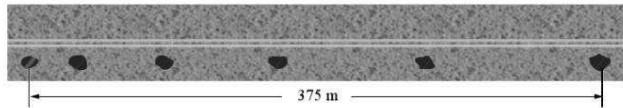
\includegraphics[width=0.5\linewidth]{figs/VN10-2022-PH-TP004-1-P-1}
	\end{center}	
	\choice
	{$\SI{12.5}{\meter/\second}$}
	{\True $\SI{15}{\meter/\second}$}
	{$\SI{30}{\meter/\second}$}
	{$\SI{25}{\meter/\second}$}
	\loigiai{Tốc độ trung bình của ô tô:
		$$v_\text{tb}=\dfrac{s}{t}=\dfrac{\SI{375}{\meter}}{\SI{25}{\second}}=\SI{15}{\meter/\second}.$$}
\end{ex}
% ===================================================================
\begin{ex}
	Một xe chuyển động thẳng không đổi chiều, $\SI{1}{\hour}$ đầu xe chạy với tốc độ trung bình $\SI{60}{\kilo\meter/\hour}$ và $\SI{3}{\hour}$ sau xe chạy với tốc độ trung bình $\SI{40}{\kilo\meter/\hour}$. Tốc độ trung bình của xe trong suốt thời gian chuyển động là
	\choice
	{$\SI{48}{\kilo\meter/\hour}$}
	{$\SI{40}{\kilo\meter/\hour}$}
	{$\SI{58}{\kilo\meter/\hour}$}
	{\True $\SI{45}{\kilo\meter/\hour}$}
	\loigiai{$$v_{tb}=\dfrac{v_1t_1+v_2t_2}{t_1+t_2}=\SI{45}{\kilo\meter/\hour}.$$}
\end{ex}
% ===================================================================
\begin{ex}
	Một người đi xe đạp trên $\dfrac{2}{3}$ đoạn đường đầu với tốc độ trung bình $\SI{10}{\kilo\meter/\hour}$ và $\dfrac{1}{3}$ đoạn đường sau với tốc độ trung bình $\SI{20}{\kilo\meter/\hour}$. Tốc độ trung bình của người đi xe đạp trên cả quãng đường là
	\choice
	{\True $\SI{12}{\kilo\meter/\hour}$}
	{$\SI{15}{\kilo\meter/\hour}$}
	{$\SI{17}{\kilo\meter/\hour}$}
	{$\SI{13.3}{\kilo\meter/\hour}$}
	\loigiai{Gọi $s$ là chiều dài đoạn đường
		$$v_{tb}=\dfrac{s}{t_1+t_2}=\dfrac{s}{\dfrac{2s}{3v_1}+\dfrac{s}{3v_2}}=\dfrac{1}{\dfrac{2}{3v_1}+\dfrac{1}{3v_2}}=\SI{12}{\kilo\meter/\hour}.$$}
\end{ex}
% ===================================================================
\begin{ex}
	Hình vẽ bên là đồ thị độ dịch chuyển - thời gian của một chiếc xe ô tô chạy từ $A$ đến $B$ trên một đường thẳng. Vận tốc của xe bằng
	\begin{center}
		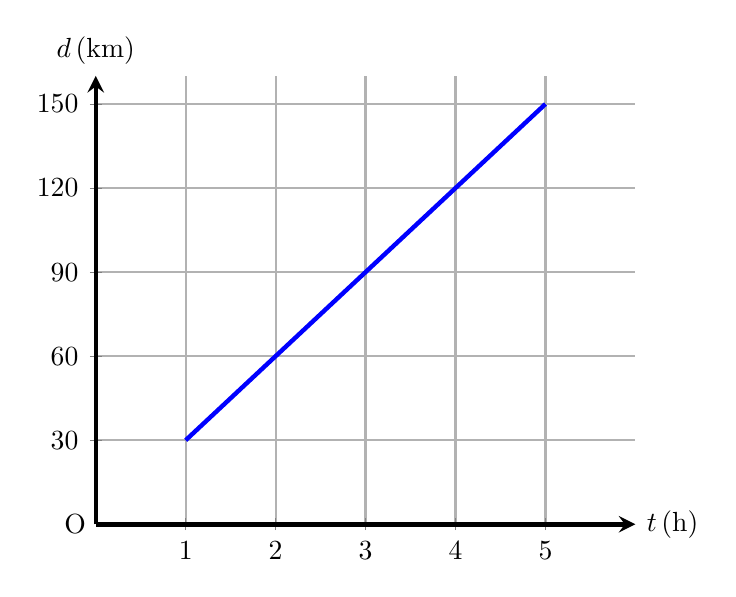
\begin{tikzpicture}  
			\begin{axis}[  ultra thick,
				xmin=0,  
				xmax=6,  
				xtick={0,1,...,5},
				ytick={0,30,...,150},
				minor x tick num=0,
				minor y tick num=0,
				ymin=0,  
				ymax=160, 
				samples=300,
				axis lines=center, 
				grid style={step=1, line width =0.4pt, color=gray!30!white},
				grid=both,
				major grid style={line width=0.8pt,gray!60!white},
				xlabel=$\xsi{t}{\left(\si{\hour}\right)}$, 		ylabel=$\xsi{d}{\left(\si{\kilo\meter}\right)}$,
				every axis y label/.style={at=(current axis.above origin),anchor=south},  
				every axis x label/.style={at=(current axis.right of origin),anchor=west},  ]
				\addplot [ultra thick, blue, smooth, domain=1:5] {30*x};			 
			\end{axis}  
			\node[left] at (0,0) {O};
		\end{tikzpicture}
	\end{center}
	\choice
	{\True $\SI{30}{\kilo\meter/\hour}$}
	{$\SI{150}{\kilo\meter/\hour}$}
	{$\SI{120}{\kilo\meter/\hour}$}
	{$\SI{100}{\kilo\meter/\hour}$}
	\loigiai{}
\end{ex}
% ===================================================================
\begin{ex}
	Một chất điểm chuyển động trên một đường thẳng. Đồ thị độ dịch chuyển theo thời gian của chất điểm được mô tả như hình vẽ. Tốc độ trung bình của chất điểm trong khoảng thời gian từ 0 đến $\SI{5}{\second}$ là
	\begin{center}
		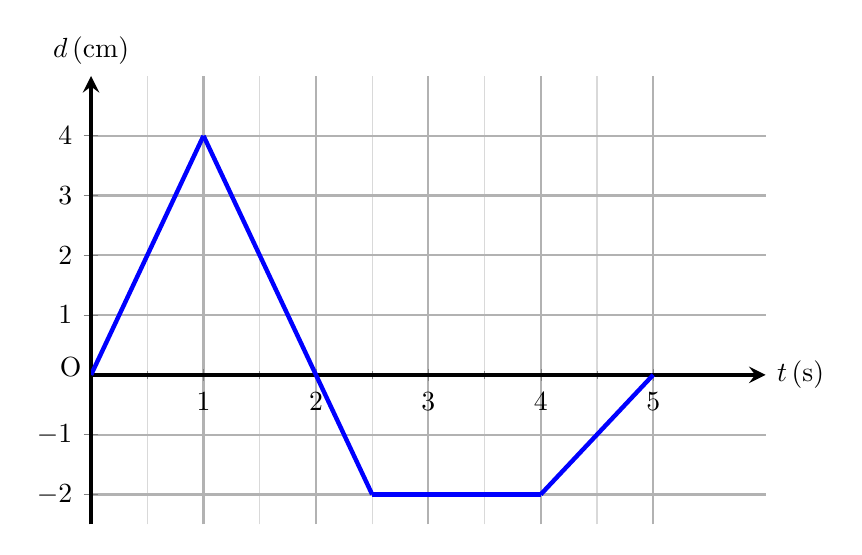
\begin{tikzpicture}  
			\begin{axis}[  ultra thick,xscale=1.25,
				xmin=0,  
				xmax=6,  
				xtick={0,1,...,5},
				ytick={-2,-1,0,1,...,4},
				minor x tick num=1,
				minor y tick num=0,
				ymin=-2.5,  
				ymax=5, 
				samples=300,
				axis lines=center, 
				grid style={step=1, line width =0.4pt, color=gray!30!white},
				grid=both,
				major grid style={line width=0.8pt,gray!60!white},
				xlabel=$\xsi{t}{\left(\si{\second}\right)}$, 		ylabel=$\xsi{d}{\left(\si{\centi\meter}\right)}$,
				every axis y label/.style={at=(current axis.above origin),anchor=south},  
				every axis x label/.style={at=(current axis.right of origin),anchor=west},  ]
				\addplot [ultra thick, blue, smooth, domain=0:1] {4*x};	
				\addplot [ultra thick, blue, smooth, domain=1:2.5] {4-4*(x-1)};		
				\addplot [ultra thick, blue, smooth, domain=2.5:4] {-2};	 
				\addplot [ultra thick, blue, smooth, domain=4:5] {-2+2*(x-4)};
				
			\end{axis}  
			\node[left] at (0,2) {O};
			
		\end{tikzpicture}
	\end{center}
	\choice
	{$\SI{1.6}{\centi\meter/\second}$}
	{$\SI{6.4}{\centi\meter/\second}$}
	{$\SI{4.8}{\centi\meter/\second}$}
	{\True $\SI{2.4}{\centi\meter/\second}$}
	\loigiai{
		Tốc độ trung bình của chất điểm:
		$$v_\text{tb}=\dfrac{s}{t}=\dfrac{4+4+2+2}{5}=\SI{2.4}{\centi\meter/\second}.$$	
	}
\end{ex}
% ===================================================================
\begin{ex}
	Đồ thị toạ độ - thời gian của hai xe (I) và (II) cùng chuyển động trên một đường thẳng được thể hiện như hình bên. Thời điểm hai xe gặp nhau là
	\begin{center}
		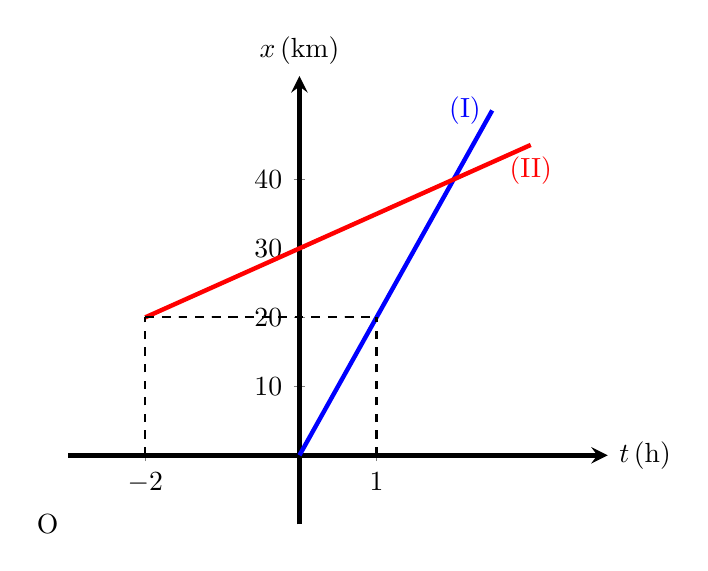
\begin{tikzpicture}  
			\begin{axis}[  ultra thick,
				xmin=-3,  
				xmax=4,  
				xtick={-2,0,1},
				ytick={0,10,...,40},
				minor x tick num=0,
				minor y tick num=0,
				ymin=-10,  
				ymax=55, 
				samples=300,
				axis lines=center, 
				xlabel=$\xsi{t}{\left(\si{\hour}\right)}$, 		ylabel=$\xsi{x}{\left(\si{\kilo\meter}\right)}$,
				every axis y label/.style={at=(current axis.above origin),anchor=south},  
				every axis x label/.style={at=(current axis.right of origin),anchor=west},  ]
				\addplot [ultra thick, blue, smooth, domain=0:2.5] {20*x} node[left] {(I)};	
				\addplot [ultra thick, red, smooth, domain=-2:3] {30+5*x} node[below] {(II)};	
				\addplot [thick, dashed, domain=-2:1] {20} ;	
				\draw[thick, dashed] (axis cs:-2,0) --(axis cs:-2,20);	 
				\draw[thick, dashed] (axis cs:1,0) --(axis cs: 1,20);
			\end{axis}  
			\node[left] at (0,0) {O};
		\end{tikzpicture}
	\end{center}
	\choice
	{$\SI{1}{\hour}$}
	{\True$\SI{2}{\hour}$}
	{$\SI{2.5}{\hour}$}
	{$\SI{1.33}{\hour}$}
	\loigiai{}
\end{ex}

% ===================================================================
\begin{ex}
	Hình dưới là đồ thị độ dịch chuyển - thời gian của hai vật chuyển động thẳng cùng hướng. Tỉ lệ vận tốc $\dfrac{v_A}{v_B}$ là
	\begin{center}
		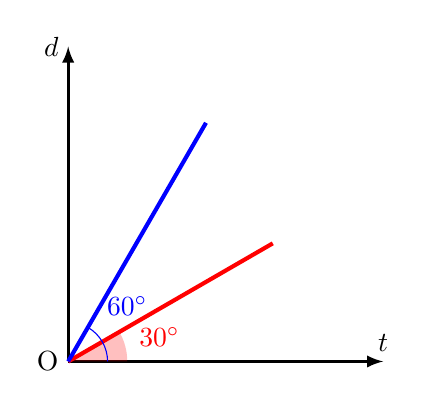
\begin{tikzpicture} 
			\coordinate (O)  at (0,0);
			\coordinate (t) at (4,0);
			\coordinate (d) at (0,4);
			\coordinate (A) at ($(O)+(30:3)$);
			\coordinate (B) at ($(O)+(60:3.5)$);
			\draw[line width=1pt, -latex] (O)--(d);
			\draw[line width=1pt, -latex] (O)--(t);
			\draw[line width=1.5pt, red] (O)--(A);
			\draw[line width=1.5pt, blue] (O)--(B);
			\node[left] at (O) {O};
			\node[above] at (t) {$t$};
			\node[left] at (d) {$d$};
			\tkzFillAngle[size=0.75cm,color=red, fill=red, opacity=0.25](t,O,A);
			\tkzLabelAngle[color=red,pos=1.2](t,O,A){$\SI{30}{\degree}$}
			\tkzMarkAngle[size=0.5cm,color=blue](t,O,B);
			\node[blue] at (0.75,0.7) {$\SI{60}{\degree}$};
		\end{tikzpicture}
	\end{center}
	\choice
	{$\dfrac{3}{1}$}
	{$\dfrac{1}{3}$}
	{$\dfrac{\sqrt{3}}{1}$}
	{$\dfrac{1}{\sqrt{3}}$}
	\loigiai{}
\end{ex}
\textbf{BÀI TẬP TỰ LUẬN}
% ======================================================================
\begin{ex}
	Lúc $\SI{7}{\hour}$ có một xe khởi hành từ A chuyển động thẳng đều về B với tốc độ $\SI{40}{\kilo\meter/\hour}$. Lúc $\SI{7}{\hour}\SI{30}{\minute}$ một xe khác khởi hành từ B chuyển động thẳng đều về A  với tốc độ $\SI{50}{\kilo\meter/\hour}$. Cho $\mathrm{AB}=\SI{110}{\kilo\meter}$.
	\begin{enumerate}[label=\alph*)]
		\item Xác định vị trí của mỗi xe và khoảng cách giữa chúng lúc $\SI{8}{\hour}$ và lúc $\SI{9}{\hour}$.
		\item Hai xe gặp nhau lúc mấy giờ? Ở đâu?
	\end{enumerate}
	\loigiai{
		\begin{enumerate}[label=\alph*)]
			\item Cách A $\SI{40}{\kilo\meter}$, $\SI{85}{\kilo\meter}$, $\SI{45}{\kilo\meter}$.\\
			Cách A $\SI{80}{\kilo\meter}$, $\SI{35}{\kilo\meter}$, $\SI{45}{\kilo\meter}$.
			\item $\SI{8}{\hour}\SI{30}{\minute}$; cách A $\SI{60}{\kilo\meter}$.
		\end{enumerate}
	}
\end{ex}
% ======================================================================
\begin{ex}
	Hai xe chuyển động trên hai đường vuông góc với nhau, xe A đi về hướng tây với tốc độ $\SI{50}{\kilo\meter/\hour}$, xe B đi về hướng Nam với tốc độ $\SI{30}{\kilo\meter/\hour}$. Vào một thời điểm nào đó xe A và B còn cách giao điểm của hai đường lần lượt là $\SI{4.4}{\kilo\meter}$ và $\SI{4}{\kilo\meter}$, hai xe đang tiến về phía giao điểm. Tìm khoảng cách ngắn nhất giữa hai xe.
	\loigiai{
		$\SI{1.166}{\kilo\meter}$.
	}
\end{ex}
\chapter{Bài 5. Chuyển động tổng hợp}
\begin{center}
	\textit{(3 tiết)}
\end{center}
\section{MỤC TIÊU DẠY HỌC}
\begin{center}
	\begin{longtable}{|M{2.5cm}|L{12.5cm}|M{2cm}|}
		\hline
		\thead{Biểu hiện\\ năng lực} & \thead{Mục tiêu} & \thead{STT}\\
		\hline
		\multicolumn{3}{|c|}{\textbf{ Năng lực vật lí}}\\
		\hline
		1.1 & Phát biểu được tính tương đối của chuyển động và vận tốc, từ đó thấy được tầm quan trọng của hệ quy chiếu. & 1\\
		\hline
		1.4 & Phân biệt được hệ quy chiếu chuyển động và hệ quy chiếu đứng yên. & 2\\
		\hline
		1.2&Xác định được độ dịch chuyển tổng hợp, vận tốc tổng hợp. & 3\\
		\hline
		\multicolumn{3}{|c|}{\textbf{Năng lực chung}}\\
		\hline
		TC - TH& Tích cực thực hiện các nhiệm vụ GV đặt ra cho các nhóm, tích cực suy luận để đưa ra câu trả lời trong quá trình GV định hướng nội dung học tập	&4 \\
		\hline
		GT - HT & Tích cực đóng góp ý kiến trong quá trình thảo luận, biết sử dụng ngôn ngữ kết hợp với các loại phương tiện phi ngôn ngữ đa dạng để trình bày các kết quả thảo luận nhóm & 5\\
		\hline
	\end{longtable}
\end{center}
\section{THIẾT BỊ DẠY HỌC VÀ HỌC LIỆU}
\begin{itemize}
	\item Tivi/máy chiếu;
	\item SGK;
\end{itemize}
\section{TIẾN TRÌNH DẠY HỌC}
\subsection{TIẾN TRÌNH}\newpage
\begin{center}
	\begin{longtable}{|L{2.75cm}|C{1.25cm}|L{5cm}|L{3.5cm}|L{4cm}|}
		\hline
		\thead{Tiến trình} & \thead{Mục\\tiêu} & \thead{Nội dung dạy học \\trọng tâm} & \thead{PP,\\ KTDH} & \thead{Phương pháp \\đánh giá}\\
		\hline
	\textbf{Hoạt động 1:} Tìm hiểu về tính tương đối của chuyển động	& 1, 2  & Tính tương đối của chuyển động. Phân biệt hệ quy chiếu chuyển động và hệ quy chiếu đứng yên.  & PPDH: Đàm thoại & GV đánh giá dựa trên câu trả lời của HS.\newline
	PP đánh giá: quan sát, nghe.  \\
		\hline
		\textbf{Hoạt động 2:} Tìm hiểu độ dịch chuyển tổng hợp - vận tốc tổng hợp. & 3 & Độ dịch chuyển tổng hợp, vận tốc tổng hợp & PPDH: Đàm thoại &  GV đánh giá dựa trên câu trả lời của HS.\newline
		PP đánh giá: quan sát, nghe.  \\
		\hline
		\textbf{Hoạt động 3:} Vận dụng quy tắc cộng vector để tìm vận tốc tổng hợp trong các trường hợp đơn giản. & 3, 4, 5 & Công thức vận tốc tổng hợp trong trường hợp: \begin{itemize}
			\item $\vec{v}_{12}\uparrow\uparrow \vec{v}_{23}$; \item $\vec{v}_{12}\uparrow\downarrow \vec{v}_{23}$; \item $\vec{v}_{12}\bot\vec{v}_{23}$
		\end{itemize}& PPDH: Dạy học hợp tác & GV đánh giá dựa trên câu trả lời đại diện nhóm HS.\newline
		PP đánh giá: quan sát, nghe.  \\
		\hline
		\textbf{Hoạt động 4:} Luyện tập	& 1, 2, 3  & Luyện tập bài tập vận tốc tổng hợp, bài toán thuyền chạy xuôi dòng/ngược dòng. & PPDH:  Đàm thoại& GV đánh giá dựa trên bài tập cá nhân của học sinh.\newline
		PP đánh giá: quan sát, nghe. \\
		\hline
		\end{longtable}
\end{center}
% ==========================================================================================
\hoatdong
{Tìm hiểu về tính tương đối của chuyển động.	
}
{\begin{itemize}
		\item HS phát biểu được tính tương đối của chuyển động và vận tốc, từ đó thấy được tầm quan trọng của hệ quy chiếu.
		\item HS phân biệt được hệ quy chiếu chuyển động và hệ quy chiếu đứng yên.
	\end{itemize}
	
}
{
		Kết quả trả lời của HS cho các câu hỏi gợi mở của GV:\\
	\textbf{Câu trả lời dự kiến:} 
	\begin{itemize}
		\item Câu hỏi 1: Khi bánh xe đạp quay, quỹ đạo chuyển động của đầu van so với trục ổ bi có hình dạng gì?\\
		Trả lời: quỹ đạo tròn.
		\item Câu hỏi 2: Đối với người quan sát bên đường, đầu van xe đạp chuyển động với quỹ đạo thế nào?\\
		Trả lời: quỹ đạo như một nửa đường xoắn ốc (cycloid).
		\item Câu hỏi 3: Nhận xét trạng thái chuyển động của hành khách so với tài xế và cây xương rồng bên đường.\\
		Trả lời: Hành khách đứng yên so với tài xế nhưng đang chuyển động so với cây bên đường.
	\end{itemize}
}
{\textit{\underline{* GV chuyển giao nhiệm vụ học tập}}\\
	GV lần lượt đặt các câu hỏi gợi mở cho HS.\\
	\textbf{Câu 1:} Khi bánh xe đạp quay, quỹ đạo chuyển động của đầu van so với trục ổ bi có hình dạng gì?
	\begin{center}
		
\includegraphics[width=0.4\linewidth]{figs/G10-BAI5-1}
	\end{center}
	\textbf{Câu 2:} Đối với người quan sát bên đường, đầu van xe đạp chuyển động với quỹ đạo thế nào?
	\begin{center}
		
\includegraphics[width=0.4\linewidth]{figs/G10-BAI5-2}
	\end{center}
	\textbf{Câu 3:} Nhận xét trạng thái chuyển động của hành khách so với tài xế và cây xương rồng bên đường.
	\begin{center}
		
\includegraphics[width=0.4\linewidth]{figs/G10-BAI5-3}
	\end{center}
	\textit{\underline{* HS thực hiện nhiệm vụ học tập}}\\
	HS tích lắng nghe, suy nghĩ.\\
	\textit{\underline{* HS báo cáo kết quả nhiệm vụ học tập}}\\
	HS tích cực trả lời câu hỏi gợi mở của GV.\\
	HS chú ý theo dõi, đặt câu hỏi.\\
	GV chỉnh lí, hợp thức hóa kiến thức.
}
% ==========================================================================================
\hoatdong
{Tìm hiểu độ dịch chuyển tổng hợp - vận tốc tổng hợp.
}
{HS xác định được độ dịch chuyển tổng hợp, từ đó rút ra được công thức vận tốc tổng hợp.
}
{\begin{itemize}
		\item HS lập luận để xác định được độ dịch chuyển tổng hợp $\vec{d}_{13}=\vec{d}_{12}+\vec{d}_{23}$.
		\item HS rút ra được công thức vận tốc tổng hợp $\vec{v}_{13}=\vec{v}_{12}+\vec{v}_{23}$.
	\end{itemize}
	
}
{\textit{\underline{* GV chuyển giao nhiệm vụ học tập}}\\
	GV đặt ra tình huống có vấn đề:\\
	Một hành khách (1) đang ở trên tàu (2) chuyển động thẳng đều trên đường ray (3). Hành khách đi dọc theo toa tàu, xác định độ dịch chuyển của hành khách so với đường ray.
	\begin{center}
		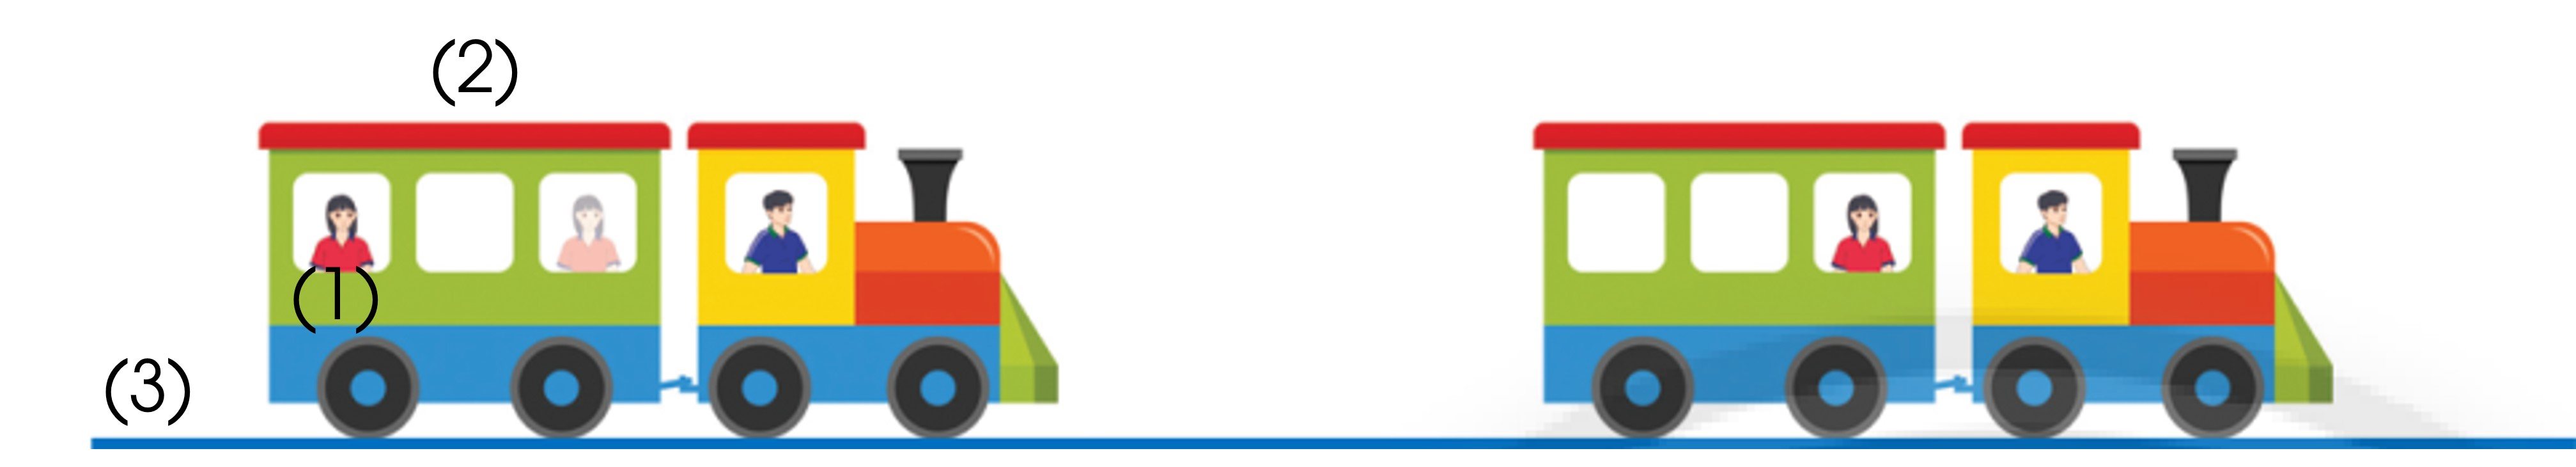
\includegraphics[width=0.7\linewidth]{figs/G10-BAI5-4}
	\end{center}
	Từ công thức độ dịch chuyển tổng hợp, GV gợi ý HS chia 2 vế của biểu thức cho $\Delta t$ để rút ra công thức vận tốc tổng hợp.\\
	\textit{\underline{* HS thực hiện nhiệm vụ học tập}}\\
	HS tích lắng nghe, suy nghĩ.\\
	\textit{\underline{* HS báo cáo kết quả nhiệm vụ học tập}}\\
	HS tích cực trả lời câu hỏi gợi mở của GV.
	\begin{center}
		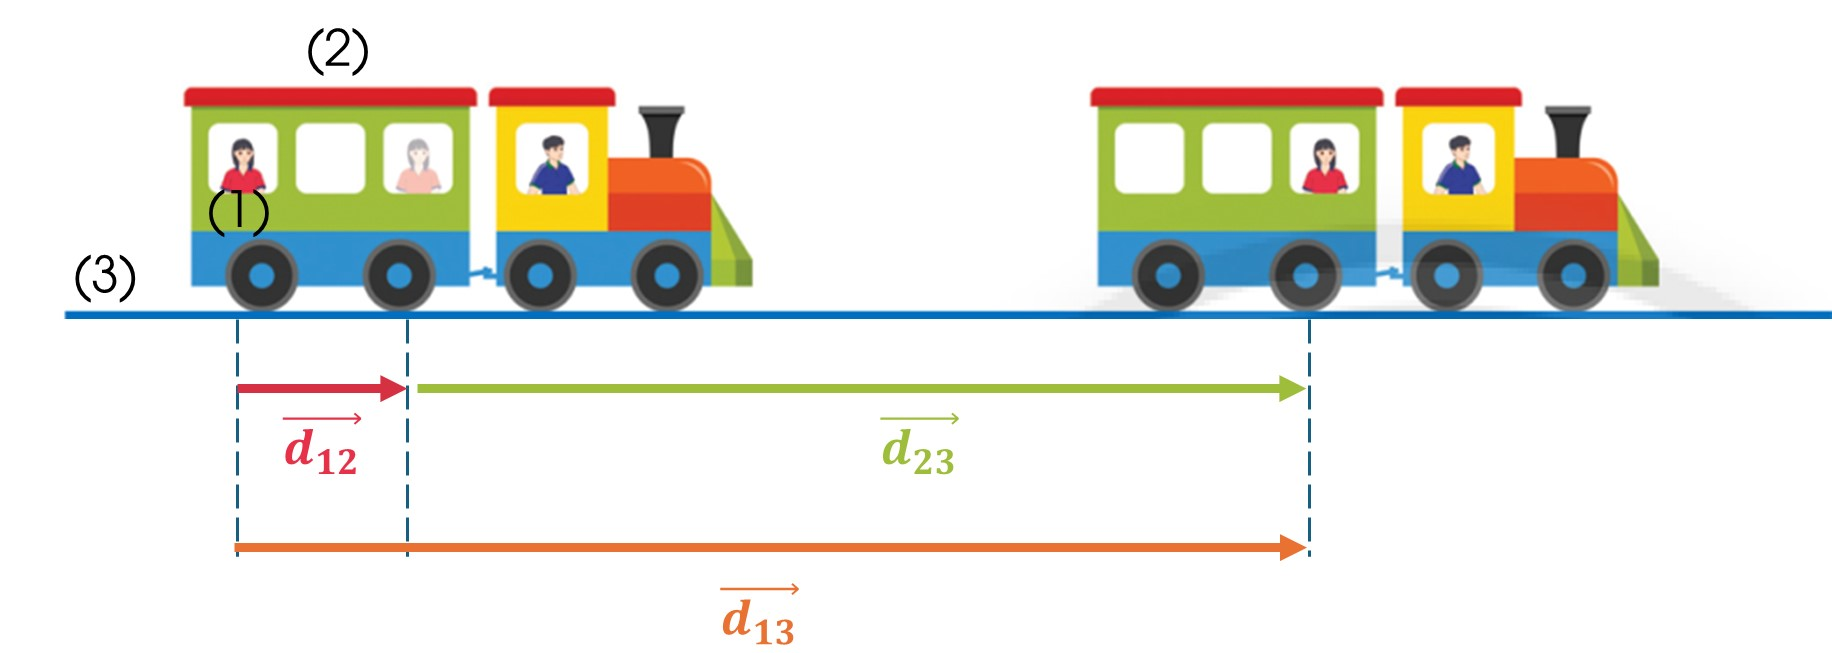
\includegraphics[width=0.7\linewidth]{figs/G10-BAI5-5}
	\end{center}
	HS chú ý theo dõi, đặt câu hỏi.\\
	GV chỉnh lí, hợp thức hóa kiến thức.
	
	
}
% ==========================================================================================
\hoatdong
{
	Vận dụng quy tắc cộng vector để tìm vận tốc tổng hợp trong các trường hợp đơn giản.
}
{
	HS vận dụng quy tắc công vector xác định được vận tốc tổng hợp trong 3 trường hợp đơn giản: $\vec{v}_{12}\uparrow\uparrow\vec{v}_{23}$; $\vec{v}_{12}\uparrow\downarrow\vec{v}_{23}$; $\vec{v}_{12}\bot\vec{v}_{23}$.
}
{HS trình bày biểu thức xác định độ lớn vận tốc tổng hợp trong 3 trường hợp đơn giản.
	\begin{center}
		\begin{tabular}{M{5.5cm}M{5.5cm}M{6cm}}
			\textbf{* Trường hợp $\vec{v}_{12}\uparrow\uparrow\vec{v}_{23}$}&\textbf{* Trường hợp $\vec{v}_{12}\uparrow\downarrow\vec{v}_{23}$}&\textbf{* Trường hợp $\vec{v}_{12}\bot\vec{v}_{23}$}\\
			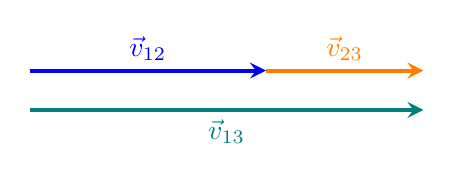
\begin{tikzpicture}
				\draw[-stealth, blue, line width=1.5pt] (0,0)--(3,0);
				\draw[-stealth, orange, line width=1.5pt] (3,0)--(5,0);
				\draw[-stealth, teal, line width=1.5pt] (0,-0.5)--(5,-0.5);
				\node[above, blue] at (1.5,0) {$\vec{v}_{12}$};
				\node[above, orange] at (4,0) {$\vec{v}_{23}$};
				\node[below, teal] at (2.5,-0.5) {$\vec{v}_{13}$};
			\end{tikzpicture}&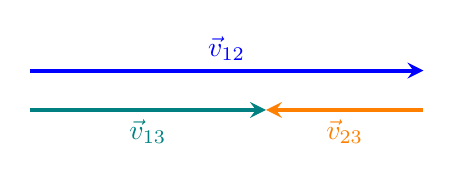
\begin{tikzpicture}
			\draw[-stealth, blue, line width=1.5pt] (0,0)--(5,0);
			\draw[-stealth, orange, line width=1.5pt] (5,-0.5)--(3,-0.5);
			\draw[-stealth, teal, line width=1.5pt] (0,-0.5)--(3,-0.5);
			\node[above, blue] at (2.5,0) {$\vec{v}_{12}$};
			\node[below, orange] at (4,-0.5) {$\vec{v}_{23}$};
			\node[below, teal] at (1.5,-0.5) {$\vec{v}_{13}$};
			\end{tikzpicture}&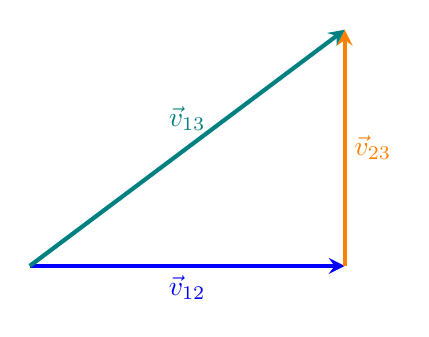
\begin{tikzpicture}
			\draw[-stealth, blue, line width=1.5pt] (0,0)--(4,0);
			\draw[-stealth, orange, line width=1.5pt] (4,0)--(4,3);
			\draw[-stealth, teal, line width=1.5pt] (0,0)--(4,3);
			\node[below, blue] at (2,0) {$\vec{v}_{12}$};
			\node[right, orange] at (4,1.5) {$\vec{v}_{23}$};
			\node[above, teal] at (2,1.6) {$\vec{v}_{13}$};
			\end{tikzpicture}\\
			 $v_{13}=v_{12}+v_{23}$&$v_{13}=\left|v_{12}-v_{23}\right|$&$v^2_{13}=v^2_{12}+v^2_{23}$
		\end{tabular}
		
	\end{center}
	HS trình bày kết quả ví dụ 1:\\
	Câu trả lời dự kiến:
	\begin{enumerate}[label=\alph*)]
		\item Hành khách đi từ cuối tàu đến đầu tàu: $v_{13}=v_{12}+v_{23}=\SI{71}{\meter/\second}$.
		\item Hành khác đi từ đầu tàu đến cuối tàu $v_{13}=\left|v_{12}-v_{23}\right|=\SI{69}{\meter/\second}$.
	\end{enumerate}
}
{\textit{\underline{* GV chuyển giao nhiệm vụ học tập}}\\
	GV ôn tập lại quy tắc hình bình hành để cộng hai vector.\\
	GV giới thiệu mở rộng cho HS quy tắc tam giác vector.\\
	GV chia lớp thành 6 nhóm.\\
	GV yêu cầu HS hoạt động theo nhóm, áp dụng quy tắc tam giác vector để xác định độ lớn vận tốc tổng hợp trong 3 trường hợp đơn giản.\\
	GV chuyển giao HS thực hiện ví dụ 1.\\
	\textit{\underline{* HS thực hiện nhiệm vụ học tập}}\\
	HS tích cực trao đổi theo nhóm.\\
	GV quan sát, hỗ trợ các nhóm gặp khó khăn.\\
	\textit{\underline{* HS báo cáo kết quả thực hiện nhiệm vụ học tập}}\\
	GV mời đại diện 3 nhóm lên bảng trình bày cho 3 trường hợp.\\
	Các nhóm còn lại nhận xét, góp ý.
	\\
	GV mời 2 HS lên bảng trình bày kết quả ví dụ 1.
	\\
	GV chỉnh lí, hợp thức hóa kiến thức.
}
\hoatdong{
	Luyện tập.
}
{
	HS xác định được vận tốc tổng hợp.\\
	HS giải được bài tập thuyền chuyển động xuôi dòng/ngược dòng.
}
{
	Bài tập cá nhân của học sinh.
}
{
	\textit{\underline{GV chuyển giao nhiệm vụ học tập}}\\
	GV lần lượt chuyển giao từng bài tập, yêu cầu HS hoạt động cá nhân để giải.\\
	\textit{\underline{HS thực hiện nhiệm vụ học tập}}\\
	HS \textit{(làm việc cá nhân)}:  Giải bài tập trong phiếu bài tập được GV giao. 
	
	GV: Theo dõi để phát hiện các HS gặp khó khăn, từ đó đưa ra sự định hướng, hỗ trợ phù hợp cho mỗi HS.\\
	\textit{\underline{HS báo cáo kết quả thực hiện nhiệm vụ học tập}}\\
	GV: Mời HS lên bảng giải bài tập.
	
	HS: Đặt câu hỏi, góp ý.
	
	GV: Chỉnh lí, hợp thức hoá kiến thức.
}
\section{HỒ SƠ DẠY HỌC}
\subsection{NỘI DUNG DẠY HỌC}
\begin{enumerate}[label=\bfseries\Roman*.]
	\item \textbf{TÍNH TƯƠNG ĐỐI CỦA CHUYỂN ĐỘNG}\\
	\begin{enumerate}[label=\bfseries\arabic*.]
		\item \textbf{Tính tương đối của vị trí}\\
		Trong các hệ quy chiếu khác nhau, vị trí của vật cũng khác nhau nên dạng quỹ đạo cũng khác nhau.
		\item \textbf{Tính tương đối của vận tốc}\\
		Trong các hệ quy chiếu khác nhau, vận tốc của vật khác nhau.
	\end{enumerate}
	$\Rightarrow$ \textbf{Vị trí và vận tốc của vật có tính tương đối.
	 }
	 \begin{itemize}
	 	\item \textbf{Hệ quy chiếu đứng yên} là hệ quy chiếu gắn với vật làm gốc được quy ước là đứng yên.
	 	\item \textbf{Hệ quy chiếu chuyển động} là hệ quy chiếu gắn với vật làm gốc chuyển động so với hệ quy chiếu đứng yên.
	 \end{itemize}
	 \item \textbf{ĐỘ DỊCH CHUYỂN TỔNG HỢP - VẬN TỐC TỔNG HỢP}\\
	 Xét vật 1 chuyển động so với vật 3 đứng yên (được chọn làm gốc của HQC đứng yên); vật 2 (được chọn làm gốc của HQC chuyển động) chuyển động so với vật 3. Ta có:\\
	 Khi vật 1 có độ dịch chuyển $\vec{d}_{12}$ so với vật 2, đồng thời vật 2 cũng có độ dịch chuyển $\vec{d}_{23}$ so với vật 3 và khi đó vật 1 có độ dịch chuyển $\vec{d}_{13}$ so với vật 3.\\
	 \textbf{Biểu thức độ dịch chuyển tổng hợp:}\\
	 $$\vec{d}_{13}=\vec{d}_{12}+\vec{d}_{23}$$
	 \textbf{Biểu thức của vận tốc tổng hợp:}
	 $$\vec{v}_{13}=\vec{v}_{12}+\vec{v}_{23}$$
	 \begin{center}
	 	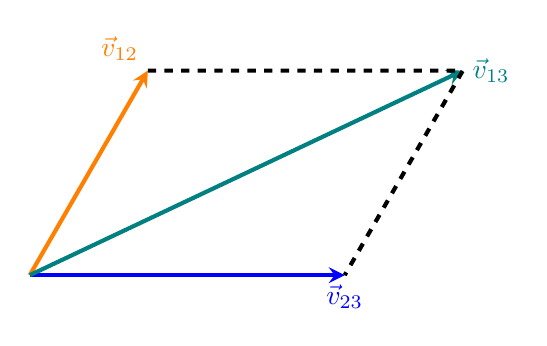
\begin{tikzpicture}
	 		\coordinate (O) at (0,0);
	 		\coordinate (A) at ($(O)+(60:3)$);
	 		\coordinate (B) at (4,0);
	 		\coordinate (C) at ($(B)+(60:3)$);
	 		\draw[-stealth, line width=1.5pt, blue] (O)--(B);
	 		\draw[-stealth, line width=1.5pt, orange] (O)--(A);
	 		\draw[-stealth, line width=1.5pt, teal] (O)--(C);
	 		\draw[ line width=1.5pt, black, dashed] (A)--(C)--(B);
	 		\node[right, teal] at (C) {$\vec{v}_{13}$};
	 		\node[below, blue] at (B) {$\vec{v}_{23}$};
	 		\node[above left, orange] at (A) {$\vec{v}_{12}$};
	 	\end{tikzpicture}
	 \end{center}
	 Trong đó:
	 \begin{itemize}
	 	\item $\vec{v}_{13}$: vận tốc của vật 1 đối với vật 3, gọi là \textbf{vận tốc tuyệt đối};
	 	\item $\vec{v}_{12}$: vận tốc của vật 1 đối với vật 2, gọi là \textbf{vận tốc tương đối};
	 	\item $\vec{v}_{23}$: vận tốc của vật 2 đối với vật 3, gọi là \textbf{vận tốc kéo theo}.
	 \end{itemize}
	 \textbf{Các trường hợp đặc biệt:}
	 \begin{itemize}
	 	\item Trường hợp $\vec{v}_{12}$ và $\vec{v}_{23}$ cùng hướng: $v_{13}=v_{12}+v_{23}$;
	 	\item Trường hợp $\vec{v}_{12}$ và $\vec{v}_{23}$ ngược hướng: $v_{13}=\left|v_{12}-v_{23}\right|$;
	 	\item Trường hợp $\vec{v}_{12}$ và $\vec{v}_{23}$ vuông góc: $v^2_{13}=v^2_{12}+v^2_{23}$.
	 \end{itemize}
\end{enumerate}
\subsection{CÁC HỒ SƠ KHÁC}
\textbf{* Các câu hỏi ví dụ}\\
\setcounter{ex}{0}
% ======================================================================
\begin{ex}
	Bên trong một tàu lửa đang chuyển động thẳng đều với tốc độ $\SI{70}{\meter/\second}$, một hành khách di chuyển trong tàu với tốc độ $\SI{1}{\meter/\second}$ so với lái tàu. Xác định tốc độ của người đối với cột đèn tín hiệu bên đường trong trường hợp:
	\begin{enumerate}[label=\alph*)]
		\item hành khách đi từ cuối tàu đến đầu tàu.
		\item hành khách đi từ đầu tàu đến cuối tàu.
	\end{enumerate}
	
	\loigiai{\begin{enumerate}[label=\alph*)]
			\item Hành khách đi từ cuối tàu đến đầu tàu: $v_{13}=v_{12}+v_{23}=\SI{71}{\meter/\second}$.
			\item Hành khác đi từ đầu tàu đến cuối tàu $v_{13}=\left|v_{12}-v_{23}\right|=\SI{69}{\meter/\second}$.
	\end{enumerate}}
\end{ex}
% ======================================================================
\begin{ex}
	Hai bến A và B nằm dọc theo một con sông, cách nhau $\SI{6}{\kilo\meter}$. Khi nước đứng yên (không chảy) thì thuyền chạy với tốc độ $\SI{5}{\kilo\meter/\hour}$. Khi nước chảy  với tốc độ $\SI{1}{\kilo\meter/\hour}$ và động cơ của thuyền vẫn hoạt động như trước thì thời gian thuyền chuyển động từ A đến B rồi trở lại A là bao nhiêu? Giả sử bỏ qua thời gian thuyền quay đầu.
	
	\loigiai{
	$\SI{2.5}{\hour}$.
	}
\end{ex}
\textbf{* Bài tập}\\
\textbf{BÀI TẬP TRẮC NGHIỆM}
\setcounter{ex}{0}
\Opensolutionfile{ans}[ans/BAI5-TN]
% ===================================================================
\begin{ex}
	Một người đi xe máy từ nhà đến bến xe bus cách nhà $\SI{6}{\kilo\meter}$ về phía Đông. Người đó tiếp tục lên xe bus đi tiếp $\SI{6}{\kilo\meter}$ về phía Bắc. Độ dịch chuyển tổng hợp của người này là	
	\choice
	{$\SI{12}{\kilo\meter}$}
	{$\SI{6}{\kilo\meter}$}
	{\True $\xsi{6\sqrt{2}}{\kilo\meter}$}
	{$\SI{72}{\kilo\meter}$}
	\loigiai{}
\end{ex}
% ===================================================================
\begin{ex}
	Gọi $\vec{v}_{12}$ là vận tốc của vật (1) so với vật (2), $\vec{v}_{23}$ là vận tốc của vật (2) so với vật (3), $\vec{v}_{13}$ là vận tốc của vật (1) so với vật (3). Hệ thức đúng là
	\choice
	{$\vec{v}_{13}=\vec{v}_{12}-\vec{v}_{23}$}
	{$\vec{v}_{13}=\vec{v}_{12}+2\vec{v}_{23}$}
	{\True $\vec{v}_{13}=\vec{v}_{12}+\vec{v}_{23}$}
	{$\vec{v}_{13}=2\vec{v}_{12}+\vec{v}_{23}$}
	\loigiai{}
\end{ex}
% ===================================================================
\begin{ex}
	Một hành khách ngồi trong xe A, nhìn qua cửa sổ thấy xe B bên cạnh và sân ga đều chuyển động như nhau. Như vậy
	\choice
	{xe A đứng yên, xe B chuyển động}
	{\True xe A chạy, xe B đứng yên}
	{xe A và xe B chạy cùng chiều}
	{xe A và xe B chạy ngược chiều}
	\loigiai{}
\end{ex}
% ===================================================================
\begin{ex}
	Hai ô tô A và B chạy cùng chiều trên cùng một đoạn đường với tốc độ $\SI{70}{\kilo\meter/\hour}$ và $\SI{65}{\kilo\meter/\hour}$. Tốc độ của ô tô A so với ô tô B bằng	
	\choice
	{$\SI{30}{\kilo\meter/\hour}$}
	{\True $\SI{5}{\kilo\meter/\hour}$}
	{$\SI{135}{\kilo\meter/\hour}$}
	{$\SI{65}{\kilo\meter/\hour}$}
	\loigiai{}
\end{ex}
% ===================================================================
\begin{ex}
	A ngồi trên một toa tàu chuyển động với tốc độ $\SI{15}{\kilo\meter/\hour}$ đang rời ga. B ngồi trên một toa tàu khác chuyển động với tốc độ $\SI{10}{\kilo\meter/\hour}$ đang đi ngược chiều vào ga. Hai đường tàu song song với nhau. Chọn chiều dương là chiều chuyển động của đoàn tàu mà A ngồi. Vận tốc của B đối với A là
	\choice
	{$\SI{-5}{\kilo\meter/\hour}$}
	{$\SI{5}{\kilo\meter/\hour}$}
	{$\SI{25}{\kilo\meter/\hour}$}
	{\True $\SI{-25}{\kilo\meter/\hour}$}
	\loigiai{}
\end{ex}
% ===================================================================
\begin{ex}
	Hai bến sông A và B cùng nằm trên một bờ sông, cách nhau $\SI{18}{\kilo\meter}$. Cho biết độ lớn vận tốc của ca nô đối với nước là $u =\SI{16.2}{\kilo\meter/\hour}$ và độ lớn vận tốc của nước đối với bờ sông là $v=\SI{5.4}{\kilo\meter/\hour}$. Thời gian để ca nô chạy xuôi dòng từ A đến B rồi lại chạy ngược dòng trở về A là	
	\choice
	{1 giờ 40 phút}
	{1 giờ 20 phút}
	{\True 2 giờ 30 phút}
	{2 giờ 10 phút}
	\loigiai{}
\end{ex}
% ===================================================================
\begin{ex}
	Ô tô A chạy thẳng về hướng Tây với độ lớn vận tốc $\SI{40}{\kilo\meter/\hour}$. Ô tô B chạy thẳng về hướng Bắc với độ lớn vận tốc $\SI{60}{\kilo\meter/\hour}$. Độ lớn vận tốc của ô tô B so với người ngồi trên ô tô A gần giá trị nào nhất sau đây?	
	\choice
	{$\SI{85}{\kilo\meter/\hour}$}
	{$\SI{90}{\kilo\meter/\hour}$}
	{$\SI{65}{\kilo\meter/\hour}$}
	{\True $\SI{75}{\kilo\meter/\hour}$}
	\loigiai{}
\end{ex}
% ===================================================================
\begin{ex}
	Một chiếc xuồng đi xuôi dòng nước từ A đến B mất 4 giờ, còn nếu đi ngược dòng nước từ B đến A mất 5 giờ. Biết vận tốc của dòng nước so với bờ sông là $\SI{4}{\kilo\meter/\hour}$. Quãng đường AB là
	\choice
	{\True $\SI{160}{\kilo\meter}$}
	{$\SI{120}{\kilo\meter}$}
	{$\SI{130}{\kilo\meter}$}
	{$\SI{150}{\kilo\meter}$}
	\loigiai{}
\end{ex}
% ===================================================================
\begin{ex}
	Một người lái xuồng máy cho xuồng chạy ngang con sông rộng $\SI{240}{\meter}$. Mũi xuồng luôn luôn vuông góc với bờ sông, nhưng do nước chảy nên xuồng sang đến bờ bên kia tại một điểm cách bến dự định $\SI{180}{\meter}$ về phía hạ lưu và xuồng đi hết 1 phút. Độ lớn vận tốc của xuồng so với bờ là
	\choice
	{$\SI{8}{\meter/\second}$}
	{$\SI{9}{\meter/\second}$}
	{$\SI{6}{\meter/\second}$}
	{\True $\SI{5}{\meter/\second}$}
	\loigiai{}
\end{ex}
% ===================================================================
\begin{ex}
	Nhà của Bách và trường nằm trên cùng một con đường nên hằng ngày Bách đều đi học bằng xe đạp từ nhà đến trường với tốc độ không đổi bằng $\SI{4}{\meter/\second}$ (khi trời lặng gió). Trong một lần Bách đạp xe từ nhà đến trường, có một cơn gió thổi ngược chiều trong khoảng thời gian $\SI{90}{\second}$ . Hình bên mô tả đồ thị độ dịch chuyển - thời gian của Bách trong 5 phút đầu tiên. Tốc độ của gió so với mặt đất là bao nhiêu?
	\begin{center}
		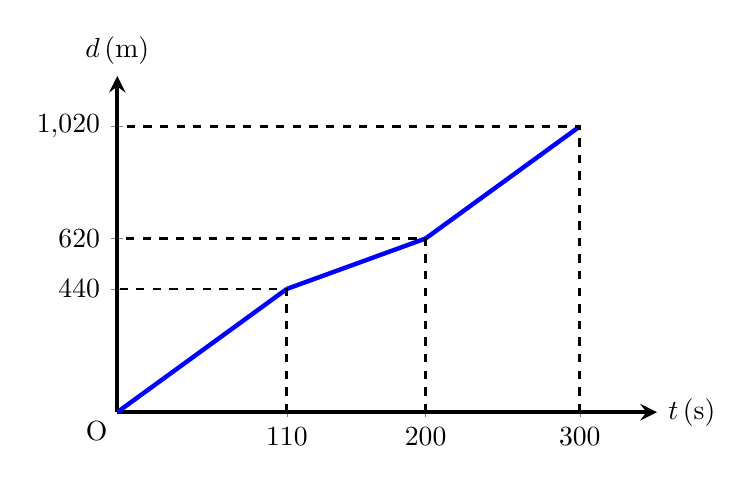
\begin{tikzpicture}  
			\begin{axis}[  ultra thick,yscale=0.75,
				xmin=0,  
				xmax=350,  
				xtick={0,110,200,300},
				ytick={0,440,620,1020},
				minor x tick num=0,
				minor y tick num=0,
				ymin=0,  
				ymax=1200, 
				samples=300,
				axis lines=center, 
				xlabel=$\xsi{t}{\left(\si{\second}\right)}$, 		ylabel=$\xsi{d}{\left(\si{\meter}\right)}$,
				every axis y label/.style={at=(current axis.above origin),anchor=south},  
				every axis x label/.style={at=(current axis.right of origin),anchor=west},  ]
				\addplot [ultra thick, blue, smooth, domain=0:110] {4*x};  
				\addplot [ultra thick, blue, smooth, domain=110:200] {440+2*(x-110)}; 
				\addplot [ultra thick, blue, smooth, domain=200:300] {620+4*(x-200)}; 
				\draw[dashed, line width=1pt] (axis cs: 110,0)--(axis cs:110,440)--(axis cs:0,440);
				\draw[dashed, line width=1pt] (axis cs: 200,0)--(axis cs:200,620)--(axis cs:0,620);
				\draw[dashed, line width=1pt] (axis cs: 300,0)--(axis cs:300,1020)--(axis cs:0,1020);
			\end{axis}  
			\node[below left] at(0,0) {O};
		\end{tikzpicture}
	\end{center}
	\choice
	{$\SI{1.2}{\meter/\second}$}
	{$\SI{1.5}{\meter/\second}$}
	{\True $\SI{2}{\meter/\second}$}
	{$\SI{2.5}{\meter/\second}$}
	\loigiai{}
\end{ex}

\Closesolutionfile{ans}
\textbf{* TỰ LUẬN}\\
\setcounter{ex}{0}
% ======================================================================
\begin{ex}
	Một ca nô chạy hết tốc lực trên mặt nước yên lặng có thể đạt $\SI{21,5}{km/h}$. Ca nô này chạy xuôi dòng sông trong 1 giờ rồi quay lại thì phải mất 2 giờ nữa mới về tới vị trí ban đầu. Hãy tính tốc độ của dòng nước.	
	\loigiai{$\SI{7.17}{\kilo\meter/\hour}$}
\end{ex}
% ======================================================================
\begin{ex}
	Một máy bay đang bay theo hướng Bắc với vận tốc $\SI{200}{m/s}$ thì bị gió từ hướng Tây thổi vào với vận tốc $\SI{20}{m/s}$. Xác định vận tốc tổng hợp của máy bay lúc này.
	\loigiai{}
\end{ex}
% ======================================================================
\begin{ex}
	Một người lái tàu vận chuyển hàng hoá xuôi dòng từ sông Đồng Nai đến khu vực cảng Sài Gòn với tốc độ là $\SI{40}{\kilo\meter/\hour}$ so với bờ. Sau khi hoàn thành công việc, lái tàu quay lại sông Đồng Nai theo lộ trình cũ với tốc độ là $\SI{30}{\kilo\meter/\hour}$ so với bờ. Biết rằng chiều và tốc độ của dòng nước đối với bờ không thay đổi trong suốt quá trình tàu di chuyển, ngoài ra tốc độ của tàu so với nước cũng được xem là không đổi. Hãy xác định tốc độ của dòng nước so với bờ.
	\loigiai{$\SI{5}{\kilo\meter/\hour}$}
\end{ex}
% ======================================================================
\begin{ex}
	Một người chèo thuyền qua một con sông rộng $\SI{400}{\meter}$. Muốn cho thuyền đi theo đường AB thì người đó phải luôn hướng mũi thuyền theo hướng AC. Biết thuyền qua sông hết $\SI{8}{\minute} \SI{20}{\second}$ và tốc độ của dòng nước là $\SI{0.6}{\meter/\second}$. Tìm tốc độ của thuyền so với dòng nước.
	\begin{center}
		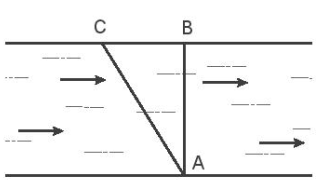
\includegraphics[width=0.35\linewidth]{figs/BAI5-1}
	\end{center}
	\loigiai{$\SI{1}{\meter/\second}$.}
\end{ex}
% ======================================================================
\begin{ex}
	Tại một thời điểm, ở vị trí M trên đoạn đường thẳng có xe máy A chạy qua với tốc độ $\SI{30}{\kilo\meter/\hour}$. Sau 10 phút, cũng tại vị trí M , có xe máy B chạy qua với tốc độ $\SI{40}{\kilo\meter/\hour}$ để đuổi theo xe máy A . Giả sử hai xe máy chuyển động thẳng với tốc độ xem như không đổi.
	\begin{enumerate}[label=\alph*)]
		\item Tính thời gian để xe máy B đuổi kịp xe máy A.
		\item Tính quãng đường mà xe máy A đã đi được đến khi xe máy B đuổi kịp.
	\end{enumerate}
	\loigiai{
		\begin{enumerate}[label=\alph*)]
			\item $\SI{0.5}{\hour}$.
			\item $\SI{15}{\kilo\meter}$.
		\end{enumerate}
	}
\end{ex}
% ======================================================================
\begin{ex}
	Một ô tô đang chạy với vận tốc $v$ theo phương nằm ngang thì người ngồi trong xe trông thấy giọt mưa rơi tạo thành những vạch làm với phương thẳng đứng một góc $\SI{45}{\degree}$. Biết vận tốc rơi của các giọt nước mưa so với mặt đất là $\SI{5}{\meter/\second}$. Tính vận tốc của ô tô.
	\loigiai{$\SI{5}{\meter/\second}$}
\end{ex}
% ======================================================================
\begin{ex}
	Một ca nô chạy ngang qua một dòng sông, xuất phát từ A , hướng mũi về B . Sau $\SI{100}{\second}$, ca nô cập bờ bên kia ở điểm C cách B $\SI{200}{\meter}$. Nếu người lái hướng mũi ca nô theo hướng AD và vẫn giữ tốc độ máy như cũ thì ca nô sẽ cập bờ bên kia tại đúng điểm B. Tìm:
	\begin{center}
		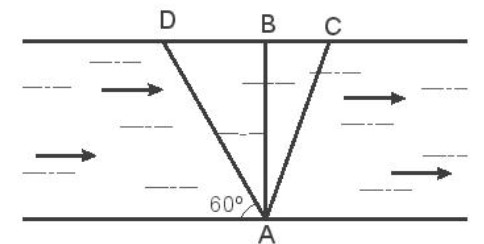
\includegraphics[width=0.35\linewidth]{figs/BAI5-2}
	\end{center}
	\begin{enumerate}[label=\alph*)]
		\item Vận tốc của dòng nước so với bờ sông.
		\item Vận tốc của ca nô so với dòng nước.
		\item Chiều rộng của sông.
	\end{enumerate}
	\loigiai{
		\begin{enumerate}[label=\alph*)]
			\item $\SI{2}{\meter/\second}$.
			\item $\SI{4}{\meter/\second}$.
			\item $\SI{400}{\meter}$.
		\end{enumerate}
	}
\end{ex}
% ======================================================================
\begin{ex}
	Hai xe chuyển động trên hai đường vuông góc với nhau, xe A đi về hướng tây với tốc độ $\SI{50}{\kilo\meter/\hour}$, xe B đi về hướng Nam với tốc độ $\SI{30}{\kilo\meter/\hour}$. Vào một thời điểm nào đó xe A và B còn cách giao điểm của hai đường lần lượt là $\SI{4.4}{\kilo\meter}$ và $\SI{4}{\kilo\meter}$, hai xe đang tiến về phía giao điểm. Tìm khoảng cách ngắn nhất giữa hai xe.\\
	\textit{(Hãy tính bài này bằng 2 cách: dùng phương pháp tọa độ và dùng vận tốc tương đối!!!)}
	\loigiai{
		$\SI{1.166}{\kilo\meter}$.
	}
\end{ex}
\begin{center}
	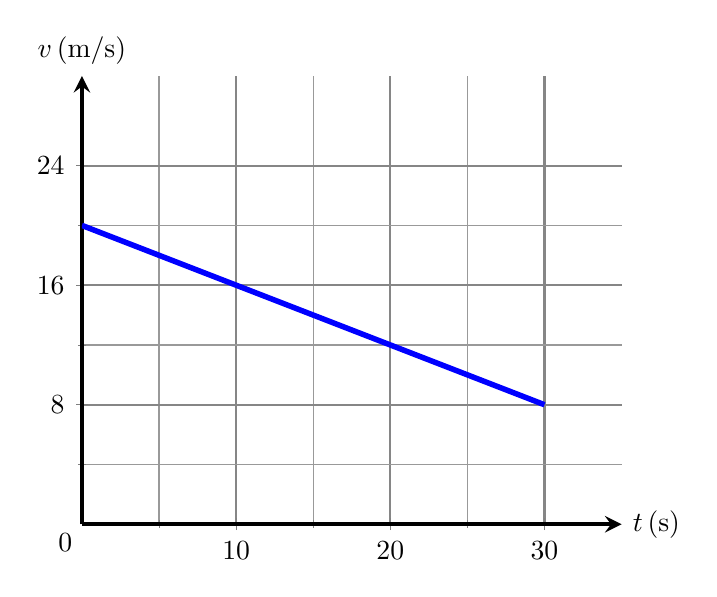
\begin{tikzpicture}  
		\begin{axis}[  ultra thick,
			xmin=0,  
			xmax=35,  
			xtick={0,10,...,30},
			ytick={0,8,...,24},
			minor x tick num=1,
			minor y tick num=1,
			ymin=0,  
			ymax=30, 
			samples=300,
			axis lines=center, 
			grid style={step=1, line width =0.4pt, color=gray!80!white},
			grid=both, %giới hạn ô lưới
			major grid style={line width=0.8pt,gray!95!white},
			xlabel=$\xsi{t}{\left(\si{\second}\right)}$, 		ylabel=$\xsi{v}{\left(\si{\meter/\second}\right)}$,
			every axis y label/.style={at=(current axis.above origin),anchor=south},  
			every axis x label/.style={at=(current axis.right of origin),anchor=west},  ]
			\addplot [line width=2pt, blue, smooth, domain=0:30] {20-0.4*x};  
			\coordinate (O) at (0,0);
		\end{axis}  
		\node[below left] at (O) {0};
	\end{tikzpicture}
\end{center}

\chapter{Bài 7. Gia tốc - Chuyển động thẳng biến đổi đều }
\begin{center}
\itshape (4 tiết)
\end{center}
\section{MỤC TIÊU DẠY HỌC}
\begin{center}
	\begin{longtable}{|M{2.5cm}|L{12.5cm}|M{2cm}|}
		\hline
		\thead{Biểu hiện\\ năng lực} & \thead{Mục tiêu} & \thead{STT}\\
		\hline
		\multicolumn{3}{|c|}{\textbf{ Năng lực vật lí}}\\
		\hline
		1.1 & Lập luận dựa vào sự biến đổi vận tốc trong chuyển động thẳng, rút ra được công thức tính gia tốc.  & 1\\
		\hline
		1.1 & Nêu được ý nghĩa, đơn vị của gia tốc.  & 2\\
		\hline
		1.2 & Dựa trên số liệu cho trước vẽ được đồ thị vận tốc – thời gian trong chuyển động thẳng. & 3\\
		\hline
		1.2 & Vận dụng đồ thị vận tốc – thời gian để tính được độ dịch chuyển và gia tốc trong một số trường hợp đơn giản. & 4\\
		\hline
		1.2 & Rút ra được các công thức của chuyển động thẳng biến đổi đều (không được dùng tích phân). & 5\\
		\hline
		1.2 & Vận dụng được các công thức của chuyển động thẳng biến đổi đều. & 6\\
		\hline
		\multicolumn{3}{|c|}{\textbf{Năng lực chung}}\\
		\hline
		GT - HT & Chủ động trong giao tiếp khi làm việc nhóm; biết khiêm tốn tiếp thu sự góp ý và nhiệt tình chia sẻ, hỗ trợ các thành viên trong nhóm. & 7\\
		\hline
		TC - TH & Chủ động, tích cực thực hiện các nhiệm vụ được đặt ra cho các nhóm; tự điều chỉnh thái độ, hành vi của bản thân, bình tĩnh và có cách cư xử đúng khi giao tiếp trong quá trình làm việc nhóm. & 8\\
		\hline
	\end{longtable}
\end{center}
\section{THIẾT BỊ DẠY HỌC VÀ HỌC LIỆU}
\begin{itemize}
	\item Tivi/máy chiếu.
	\item Phiếu thảo luận nhóm.
\end{itemize}
\section{TIẾN TRÌNH DẠY HỌC}
\subsection{TIẾN TRÌNH}
\begin{center}
	\begin{longtable}{|L{2.75cm}|C{1.25cm}|L{5cm}|L{3.5cm}|L{4cm}|}
		\hline
		\thead{Tiến trình} & \thead{Mục\\tiêu} & \thead{Nội dung dạy học \\trọng tâm} & \thead{PP,\\ KTDH} & \thead{Phương pháp \\đánh giá}\\
		\hline
		\textbf{Hoạt động 1:} Tìm hiểu khái niệm và ý nghĩa của gia tốc. & 1, 2, 7, 8 & Công thức tính gia tốc, ý nghĩa và đơn vị của gia tốc.&PP: Dạy học giải quyết vấn đề, thuyết trình. & GV đánh giá dựa trên kết quả báo cáo thảo luận nhóm của HS.\newline
		PP đánh giá: quan sát, nghe.\\
		\hline
		\textbf{Hoạt động 2:} Vận dụng đồ thị vận tốc – thời gian để tính độ dịch chuyển và gia tốc. & 3, 4, 7, 8 & Đồ thị vận tốc – thời gian trong chuyển động thẳng biến đổi đều.\newline
		Vận dụng đồ thị vận tốc – thời gian để tính độ dịch chuyển và gia tốc trong trường hợp đơn giản.
		& PP dạy học: Dạy học hợp tác, thuyết trình.\newline
		KTDH: Chia sẻ cặp đôi.
		& GV đánh giá dựa trên kết quả trên phiếu học tập và bài báo cáo của nhóm HS.\newline
		PP đánh giá: quan sát, nghe.\\
		\hline
		\textbf{Hoạt động 3:} Rút ra các công thức của chuyển động thẳng biến đổi đều. & 5, 7, 8 & Các công thức chuyển động thẳng biến đổi đều. & PP: Dạy học hợp tác. & GV đánh giá dựa trên kết quả hoạt động nhóm của HS trên phiếu học tập.\newline
		PP đánh giá: quan sát, nghe.\\
		\hline
		\textbf{Hoạt động 4:} Luyện tập. & 3, 4, 6 & Vận dụng các công thức chuyển động thẳng biến đổi đều. & PP: Đàm thoại & GV đánh giá dựa trên bài tập cá nhân của HS.\newline
		PP đánh giá: quan sát.\\
		\hline
	\end{longtable}
\end{center}
\subsection{CÁC HOẠT ĐỘNG HỌC}
\hoatdong{
Tìm hiểu khái niệm và ý nghĩa của gia tốc
}
{HS rút ra được công thức tính gia tốc.
	
HS nêu được ý nghĩa và đơn vị của gia tốc.
}
{
Phiếu hoạt động nhóm số 1 + Phần trình bày của nhóm HS.
}
{
\textit{\underline{* GV chuyển giao nhiệm vụ học tập}}\\
GV chia lớp thành 4 nhóm. GV yêu cầu HS đọc kĩ nhiệm vụ của hoạt động 1 và thảo luận theo nhóm đã chia. Sau 10 phút, GV gọi 1 nhóm lên trình bày kết quả thảo luận của nhóm, các nhóm còn lại góp ý/bổ sung.\\
\textit{\underline{* HS thực hiện nhiệm vụ học tập}}\\
HS \textit{(làm việc theo nhóm)}: Tiến hành thảo luận, đưa ra đáp án + lời giải thích cho mỗi tình huống trong phiếu học tập số 1. Nhóm HS trình bày kết quả vào phiếu học tập và thống nhất chọn đại diện báo cáo.\\
GV: Theo dõi các nhóm thảo luận để phát hiện kịp thời vấn đề mà nhóm HS gặp phải, từ đó đưa ra sự định hướng, hỗ trợ phù hợp cho mỗi nhóm.\\
\textit{\underline{* HS báo cáo kết quả thực hiện nhiệm vụ học tập}}\\
GV: Yêu cầu đại diện của 1 nhóm HS lên trình bày kết quả hoạt động 1. Các nhóm còn lại chú ý theo dõi để nhận xét.

HS: Đặt câu hỏi, góp ý.

GV: Chỉnh lí, hợp thức hoá kiến thức.

GV: Từ kết quả báo cáo của HS, GV giới thiệu khái niệm và ý nghĩa của gia tốc.

HS: Ghi chép nội dung trọng tâm vào vở.
}
%%%%%%%%%%%%%%%%%%%%%%%%%%%%%%%%%%%%%%%%%%%%%%%%%%%%%%%%%%%%%%%
\hoatdong{
Vận dụng đồ thị vận tốc – thời gian để tính độ dịch chuyển và gia tốc
}
{
	HS vận dụng đồ thị vận tốc – thời gian để tính được độ dịch chuyển và gia tốc trong một số trường hợp đơn giản.
}
{
Phiếu hoạt động nhóm số 2 + Phần trình bày của HS.
}
{
\textit{\underline{GV chuyển giao nhiệm vụ học tập}}\\
GV hướng dẫn HS cách xác định độ dịch chuyển từ đồ thị vận tốc – thời gian.

GV chia lớp thành các nhóm đôi. Một nửa số nhóm thực hiện câu a, các nhóm còn lại thực hiện câu b. 

GV yêu cầu HS đọc kĩ nhiệm vụ của hoạt động 2 và thảo luận theo nhóm đã chia. Sau 10 phút, GV gọi 2 HS đại diện của 2 nhóm lên trình bày kết quả hoạt động, các nhóm còn lại góp ý/bổ sung.\\
\textit{\underline{HS thực hiện nhiệm vụ học tập}}\\
HS \textit{(làm việc theo nhóm đôi)}: Tiến hành thảo luận, đưa ra đáp án trong phiếu học tập số 2. 

GV: Theo dõi để phát hiện các HS gặp khó khăn, từ đó đưa ra sự định hướng, hỗ trợ phù hợp cho mỗi HS.\\
\textit{\underline{HS báo cáo kết quả thực hiện nhiệm vụ học tập}}\\
GV: Yêu cầu đại diện của 2 nhóm HS lên trình bày kết quả hoạt động 2. Các nhóm còn lại chú ý theo dõi để nhận xét.

HS: Đặt câu hỏi, góp ý.

GV: Chỉnh lí, hợp thức hoá kiến thức.


}
%%%%%%%%%%%%%%%%%%%%%%%%%%%%%%%%%%%%%%%%%%%%%%%%%%%%%%%%%%%
\hoatdong{
Rút ra các công thức của chuyển động thẳng biến đổi đều.
}
{
HS vận dụng đồ thị vận tốc – thời gian để rút ra công thức tính độ dịch chuyển trong chuyển động thẳng biến đổi đều.
}
{
	Phiếu hoạt động nhóm số 3 + Phần trình bày của HS.
}
{
\textit{\underline{* GV chuyển giao nhiệm vụ học tập}}\\
GV yêu cầu HS hoạt động theo nhóm lớn đã chia và đọc kĩ nhiệm vụ của hoạt động 3. Sau 10 phút, GV gọi 1 HS đại diện của 1 nhóm lên trình bày kết quả hoạt động, các nhóm còn lại góp ý/bổ sung.\\
\textit{\underline{* HS thực hiện nhiệm vụ học tập}}
HS (làm việc theo nhóm lớn): Tiến hành thảo luận, đưa ra đáp án trong phiếu học tập số 3. 

GV: Theo dõi để phát hiện các HS gặp khó khăn, từ đó đưa ra sự định hướng, hỗ trợ phù hợp cho mỗi HS.\\
\textit{\underline{* HS báo cáo kết quả thực hiện nhiệm vụ học tập}}\\
GV: Yêu cầu đại diện của 1 nhóm HS lên trình bày kết quả hoạt động 3. Các nhóm còn lại chú ý theo dõi để nhận xét.

HS: Đặt câu hỏi, góp ý.

GV: Chỉnh lí, hợp thức hoá kiến thức.
}
%%%%%%%%%%%%%%%%%%%%%%%%%%%%%%%%%%%%%%%%%%%%%
\hoatdong{
Luyện tập.
}
{
HS vận dụng được các công thức của chuyển động thẳng biến đổi đều.
}
{
Bài tập cá nhân của học sinh.
}
{
\textit{\underline{GV chuyển giao nhiệm vụ học tập}}\\
GV lần lượt chuyển giao từng bài tập, yêu cầu HS hoạt động cá nhân để giải.\\
\textit{\underline{HS thực hiện nhiệm vụ học tập}}\\
HS \textit{(làm việc cá nhân)}:  Giải bài tập trong phiếu bài tập được GV giao. 

GV: Theo dõi để phát hiện các HS gặp khó khăn, từ đó đưa ra sự định hướng, hỗ trợ phù hợp cho mỗi HS.\\
\textit{\underline{HS báo cáo kết quả thực hiện nhiệm vụ học tập}}\\
GV: Mời HS lên bảng giải bài tập.

HS: Đặt câu hỏi, góp ý.

GV: Chỉnh lí, hợp thức hoá kiến thức.
}

\section{HỒ SƠ DẠY HỌC}
\subsection{NỘI DUNG DẠY HỌC}
\begin{enumerate}[label=\bfseries\arabic*.]
	\item \textbf{Gia tốc}\\
	Gia tốc là đại lượng đặc trưng cho độ biến thiên của vận tốc theo thời gian. Trong chuyển động thẳng, gia tốc trung bình được xác định theo biểu thức:
	\begin{equation}
		a_{tb}=\dfrac{\Delta v}{\Delta t}=\dfrac{v-v_0}{\Delta t}
	\end{equation}
	Trong hệ SI, đơn vị của gia tốc là $\si{\meter/\second^2}$.\\
	Khi $\Delta t$ rất nhỏ, gia tốc trung bình trở thành gia tốc tức thời. Gia tốc tức thời tại một thời điểm có giá trị bằng độ dốc của tiếp tuyến của đồ thị vận tốc – thời gian.\\
	Dựa vào gia tốc tức thời, ta có thể phân chuyển động thẳng thành 3 loại:
	\begin{center}
		\begin{tabular}{|M{5cm}|M{5cm}|M{6cm}|}
			\hline
			Chuyển động thẳng đều & Chuyển động thẳng biến đổi đều & Chuyển động thẳng biến đổi phức tạp\\
			\hline
			$a=0$ & $a=const\neq0$ & $a\neq0$ nhưng không phải hằng số\\
			\hline
		\end{tabular}
	\end{center}
	\item \textbf{Đồ thị vận tốc - thời gian}\\
	\begin{enumerate}[label=\bfseries \itshape 2.\arabic*., nolistsep]
		\item  \textbf{\textit{Đồ thị vận tốc – thời gian của chuyển động thẳng biến đổi đều}}\\
		Chuyển động thẳng biến đổi đều là chuyển động thẳng mà vận tốc có độ lớn tăng đều hoặc giảm đều theo thời gian:
		\begin{itemize}
			\item chuyển động thẳng có độ lớn vận tốc tăng đều theo thời gian gọi là chuyển động thẳng nhanh dần đều ( $\vec{a}\uparrow\uparrow\vec{v}$ hay $a\cdot v>0$);
			\item chuyển động thẳng có độ lớn vận tốc giảm dần theo thời gian gọi là chuyển động thẳng chậm dần đều ($\vec{a}\uparrow\downarrow\vec{v}$  hay  $a\cdot v<0$).
			
		\end{itemize}
		Nếu tại thời điểm $t_0=0$   vật có vận tốc $v_0$ thì phương trình vận tốc của vật tại thời điểm $t$:
		\begin{equation}
			v=v_0+at
		\end{equation}
		Đồ thị vận tốc – thời gian của vật chuyển động thẳng biến đổi đều có dạng:
		\begin{center}
			\begin{tabular}{M{8.5cm}M{8.5cm}}
				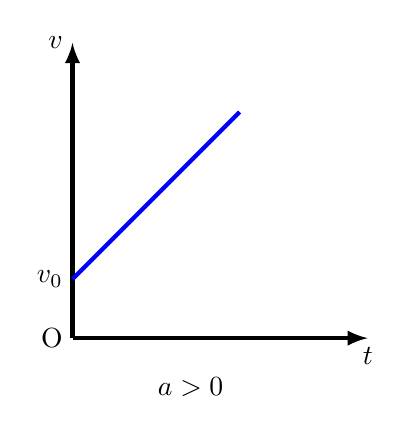
\begin{tikzpicture}[scale=0.75]  
					\coordinate (O) at(0,0);
					\coordinate (x) at(5,0);
					\coordinate (y) at(0,5);
					\coordinate (v0) at(0,1);
					\draw[-latex, line width=1.5pt] (O)--(x);
					\draw[-latex, line width=1.5pt] (O)--(y);
					\draw[blue, line width=1.5pt] (v0)--+(45:4);
					\node[below] at(x) {$t$};
					\node[left] at(y) {$v$};
					\node[left] at(v0) {$v_0$};
					\node[left] at(O) {O};
					\node[below] at (2,-0.5) {$a>0$};
				\end{tikzpicture}
				&
				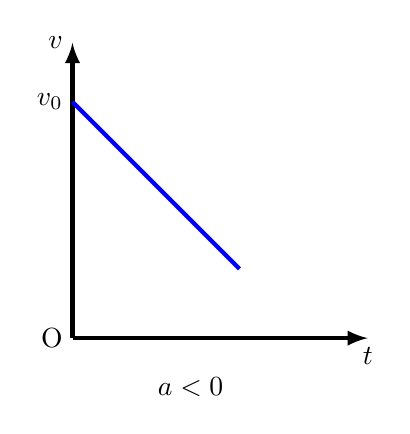
\begin{tikzpicture}  [scale=0.75] 
					\coordinate (O) at(0,0);
					\coordinate (x) at(5,0);
					\coordinate (y) at(0,5);
					\coordinate (v0) at(0,4);
					\draw[-latex, line width=1.5pt] (O)--(x);
					\draw[-latex, line width=1.5pt] (O)--(y);
					\draw[blue, line width=1.5pt] (v0)--+(-45:4);
					\node[below] at(x) {$t$};
					\node[left] at(y) {$v$};
					\node[left] at(v0) {$v_0$};
					\node[left] at(O) {O};
					\node[below] at (2,-0.5) {$a<0$};
				\end{tikzpicture}
			\end{tabular}
		\end{center}
		\item \textbf{\textit{Vận dụng độ thị vận tốc – thời gian để tính độ dịch chuyển}}\\
		\begin{center}
			\begin{tabular}{M{8cm}M{8cm}}
				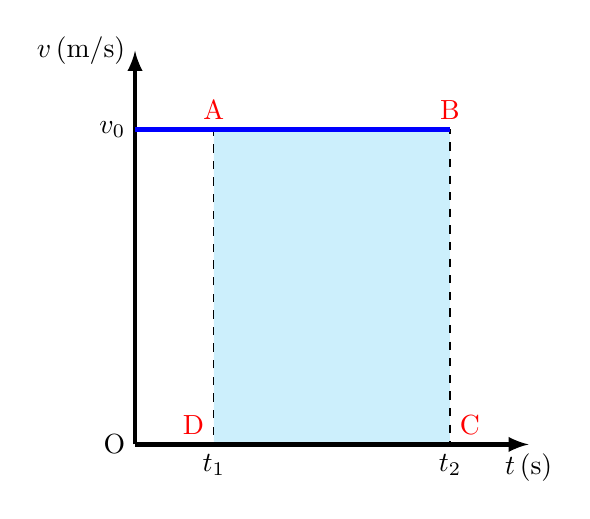
\begin{tikzpicture}  
					\coordinate (O) at(0,0);
					\coordinate (x) at(5,0);
					\coordinate (y) at(0,5);
					\coordinate (v0) at(0,4);
					\coordinate (A) at(1,4);
					\coordinate (B) at(4,4);
					\coordinate (C) at(4,0);
					\coordinate (D) at(1,0);
					\draw[-latex, line width=1.5pt] (O)--(y);
					\fill[cyan, opacity=0.2] (A)--(B)--(C)--(D)--(A);
					\draw[line width=0.5pt,black, dashed] (A)--(B)--(C)--(D)--(A);
					\draw[-latex, line width=1.5pt] (O)--(x);
					\draw[blue, line width=1.5pt] (v0)--(B);
					\node[below] at(x) {$\xsi{t}{\left(\second\right)}$};
					\node[left] at(y) {$\xsi{v}{(\meter/\second)}$};
					\node[left] at(v0) {$v_0$};
					\node[left] at(O) {O};
					\node[below] at (C) {$t_2$};
					\node[below] at (D) {$t_1$};
					\node[above, red] at(A) {A};
					\node[above, red] at(B) {B};
					\node[above right, red] at(C) {C};
					\node[above left, red] at(D) {D};
				\end{tikzpicture}
				&
				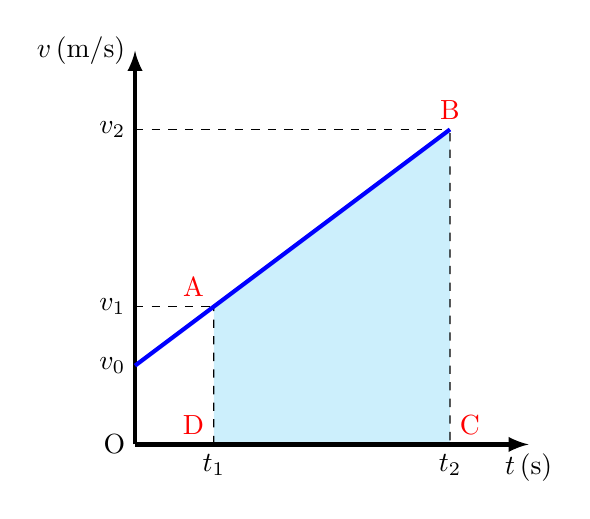
\begin{tikzpicture}  
					\coordinate (O) at(0,0);
					\coordinate (x) at(5,0);
					\coordinate (y) at(0,5);
					\coordinate (v0) at(0,1);
					\coordinate (v1) at(0,1.75);
					\coordinate (v2) at(0,4);
					\coordinate (B) at(4,4);
					\coordinate (A) at(1,1.75);
					\coordinate (C) at(4,0);
					\coordinate (D) at(1,0);
					\fill[cyan, opacity=0.2] (A)--(B)--(C)--(D)--(A);
					\draw[line width=0.5pt,black, dashed] (A)--(B)--(C)--(D)--(A);
					\draw[line width=0.5pt, dashed] (v1)--(A);
					\draw[line width=0.5pt, dashed] (v2)--(B);
					\draw[-latex, line width=1.5pt] (O)--(x);
					\draw[-latex, line width=1.5pt] (O)--(y);
					\draw[blue, line width=1.5pt] (v0)--(B);
					\node[below] at(x) {$\xsi{t}{\left(\second\right)}$};
					\node[left] at(y) {$\xsi{v}{(\meter/\second)}$};
					\node[left] at(v0) {$v_0$};
					\node[left] at(v1) {$v_1$};
					\node[left] at(0,4) {$v_2$};
					\node[left] at(O) {O};
					\node[below] at (C) {$t_2$};
					\node[below] at (D) {$t_1$};
					\node[above left, red] at(A) {A};
					\node[above, red] at(B) {B};
					\node[above right, red] at(C) {C};
					\node[above left, red] at(D) {D};
				\end{tikzpicture}\\
				Đồ thị $v-t$ trong chuyển động\newline thẳng đều. & Đồ thị $v-t$ trong chuyển động \newline thẳng biến đổi đều.
			\end{tabular}
		\end{center}
		Độ dịch chuyển của vật trong khoảng thời gian từ $t_1$ đến $t_2$ được xác định bằng phần diện tích giới hạn bởi các đường $v\left(t\right)$, $v=0$ , $t=t_1$, $t=t_2$  trong đồ thị $\left(v-t\right)$.
	\end{enumerate}
	\item \textbf{Các phương trình của chuyển động thẳng biến đổi đều}\\
	\begin{itemize}[topsep=0pt]
		\item Phương trình gia tốc: $a=const$;
		\item Phương trình vận tốc: $v=v_0+at$ với $v=v_0$ khi $t_0=0$;
		\item Phương trình quãng đường: $s=v_0t+\dfrac{1}{2}at^2$;
		\item Phương trình toạ độ: $x=x_0+v_0t+\dfrac{1}{2}at^2$;
		\item Phương trình độc lập thời gian:
		$v^2-v^2_0=2as$.
	\end{itemize}
\end{enumerate}
\subsection{CÁC  HỒ SƠ KHÁC}
Phiếu học tập\newpage
\textbf{* Phiếu số 1:} Tìm hiểu khái niệm và ý nghĩa của gia tốc.
\begin{center}
	\begin{longtable}{|L{8.5cm}L{8.5cm}|}
		\hline
		\multicolumn{2}{|c|}{\thead{PHIẾU HỌC TẬP SỐ 1 (NHÓM LỚN)\\	TÌM HIỂU KHÁI NIỆM VÀ Ý NGHĨA GIA TỐC
		}}\\
		\hline
		Lớp: \dotfill & Nhóm: \dotfill\\
		\multicolumn{2}{|l|}{Tên: \dotfill}\\
		\hline
		\multicolumn{2}{|L{17cm}|}{\textbf{Nhiệm vụ:} Trong mỗi tình huống sau đây, hãy chỉ ra đối tượng có khả năng tăng tốc hiệu quả hơn (khả năng tăng tốc nhanh hơn) và đưa ra lời giải thích cho lựa chọn của em?}\\
		\hline
		\multicolumn{2}{|c|}{\textbf{Tình huống 1}}\\
		\multicolumn{2}{|L{17cm}|}{
			\begin{itemize}[topsep=0pt]
				\item Báo guépard có khả năng tăng tốc từ $\SI{0}{\kilo\meter/\hour}$ lên $\SI{96}{\kilo\meter/\hour}$ trong thời gian $\SI{3}{\second}$.
				\item Xe đua F1 có khả năng tăng tốc từ $\SI{0}{\meter/\second}$  lên $\SI{25}{\meter/\second}$  trong khoảng thời gian $\SI{3}{\second}$.
			\end{itemize}	
			\begin{center}
				\begin{tabular}{M{6cm}M{2cm}M{6cm}}
						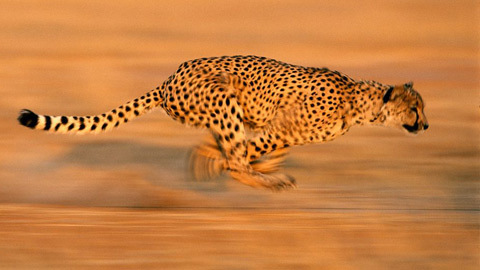
\includegraphics[scale=0.3]{figs/G10-BAI7-1}& & 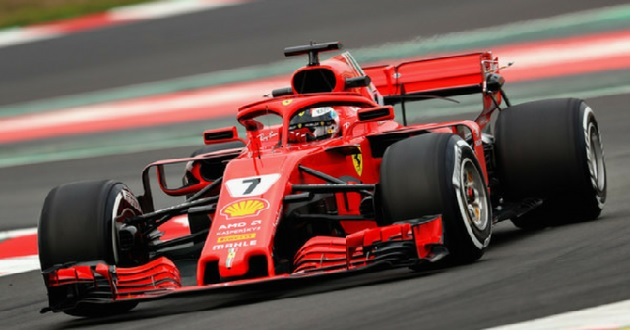
\includegraphics[scale=0.3]{figs/G10-BAI7-2}\\
						Báo guépard && Xe đua F1\\
				\end{tabular}
			\end{center}
			\dotfill
		}\\
		\multicolumn{2}{|L{17cm}|}{
			\dotfill
		}\\
		
		\multicolumn{2}{|L{17cm}|}{
			\dotfill
		}\\
		\hline
		\multicolumn{2}{|c|}{\textbf{Tình huống 2}}\\
		\multicolumn{2}{|L{17cm}|}{
			\begin{itemize}[topsep=0pt]
				\item Xe Porsche 911 Turbo S Lightweight 2021 có khả năng tăng tốc từ  $\SI{0}{\kilo\meter/\hour}$ lên $\SI{96}{\kilo\meter/\hour}$  trong thời gian $\SI{2.1}{\second}$.
				\item Xe Lamborghini Huracan Performante có khả năng tăng tốc từ $\SI{0}{\kilo\meter/\hour}$  lên $\SI{96}{\kilo\meter/\hour}$  trong thời gian $\SI{2.2}{\second}$.
			\end{itemize}	
			\begin{center}
				\begin{tabular}{M{6cm}M{2cm}M{6cm}}
					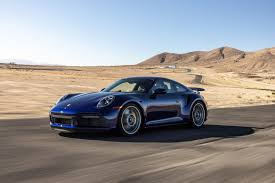
\includegraphics[scale=0.5]{figs/G10-BAI7-3}& & 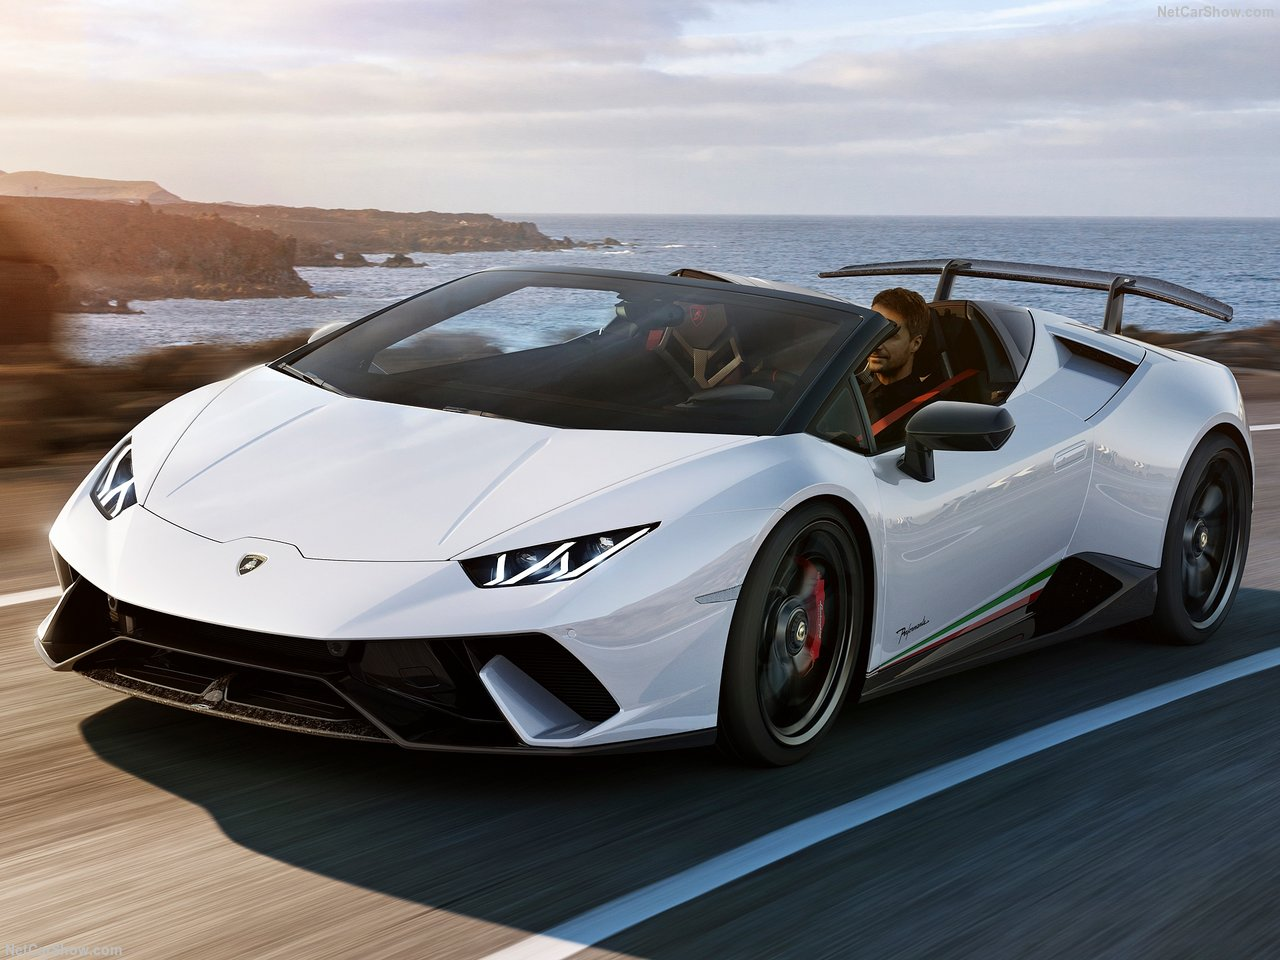
\includegraphics[scale=0.1]{figs/G10-BAI7-4}\\
					Xe Porsche 911 Turbo S Lightweight 2021 && Xe Lamborghini Huracan Performante\\
				\end{tabular}
			\end{center}
			\dotfill
		}\\
		\multicolumn{2}{|L{17cm}|}{
			\dotfill
		}\\
		
		\multicolumn{2}{|L{17cm}|}{
			\dotfill
		}\\
		\hline
		\multicolumn{2}{|c|}{\textbf{Tình huống 3}}\\
		\multicolumn{2}{|L{17cm}|}{
			\begin{itemize}[topsep=0pt]
				\item Vận động viên A từ khi xuất phát đến khi đạt tốc độ $\SI{9}{\meter/\second}$  mất thời gian $\SI{2}{\second}$.
				\item Vận động viên B từ khi xuất phát đến khi đạt tốc độ $\SI{6}{\meter/\second}$  mất thời gian $\SI{1.5}{\second}$.
			\end{itemize}	
			\dotfill
		}\\
		\multicolumn{2}{|L{17cm}|}{
			\dotfill
		}\\
		
		\multicolumn{2}{|L{17cm}|}{
			\dotfill
		}\\
		\multicolumn{2}{|L{17cm}|}{
			\dotfill
		}\\
		\hline
	\end{longtable}
\end{center}
\textbf{Phiếu số 2:} Vận dụng đồ thị $v-t$ để xác định độ dịch chuyển và gia tốc.
\begin{center}
	\begin{longtable}{|L{8.5cm}|L{8.5cm}|}
		\hline
		\multicolumn{2}{|M{17cm}|}{\bfseries PHIẾU HỌC TẬP SỐ 2 \textit{(NHÓM ĐÔI)}\newline
			VẬN DỤNG ĐỒ THỊ  ĐỂ XÁC ĐỊNH ĐỘ DỊCH CHUYỂN VÀ GIA TỐC
		}\\
		\hline
		\multicolumn{2}{|M{17cm}|}{Lớp: \dotfill}\\
		\multicolumn{2}{|M{17cm}|}{Nhóm: \dotfill}\\
		\multicolumn{2}{|M{17cm}|}{Tên: \dotfill}\\
		\hline
		\multicolumn{2}{|L{17cm}|}{
			\textbf{Nhiệm vụ:}	Dựa vào đồ thị $\left(v-t\right)$ của vật chuyển động trong hình, hãy xác định gia tốc và độ dịch chuyển của vật trong các giai đoạn:
			\begin{center}
				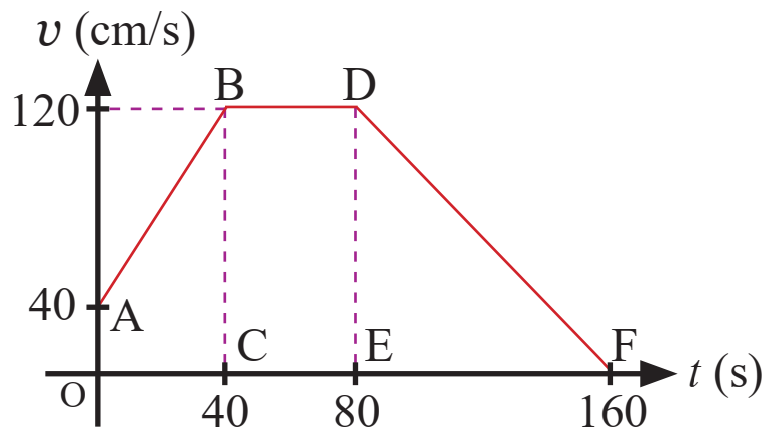
\includegraphics[width=0.4\linewidth]{../figs/BAI7-1}
			\end{center}
		}\\
		a) Từ $\SI{0}{\second}$ đến $\SI{40}{\second}$ & b) Từ $\SI{80}{\second}$ đến $\SI{160}{\second}$\\
		\dotfill & \dotfill \\
		\dotfill & \dotfill \\
		\dotfill & \dotfill \\
		\dotfill & \dotfill \\
		\dotfill & \dotfill \\
		\hline
	\end{longtable}
\end{center}
\newpage
\textbf{Phiếu số 3:} Rút ra được công thức độ dịch chuyển trong chuyển động thẳng biến đổi đều.
\begin{center}
	\begin{longtable}{|L{8.5cm}L{8.5cm}|}
		\hline
		\multicolumn{2}{|M{17cm}|}{\textbf{PHIẾU HỌC TẬP SỐ 3 \textit{(NHÓM LỚN)}	RÚT RA ĐƯỢC CÔNG THỨC\newline ĐỘ DỊCH CHUYỂN TRONG CHUYỂN ĐỘNG THẲNG BIẾN ĐỔI ĐỀU
		}}\\
		\hline
		Lớp: \dotfill & Nhóm: \dotfill\\
		\multicolumn{2}{|L{17cm}|}{Tên: \dotfill}\\
		\hline
		\multicolumn{2}{|L{17cm}|}{\textbf{Nhiệm vụ:} Dựa vào đồ thị $\left(v-t\right)$ của vật chuyển động thẳng biến đổi đều, hãy rút ra công thức xác định độ dịch chuyển theo $v_0$ , $a$, $t$.
			\begin{center}
				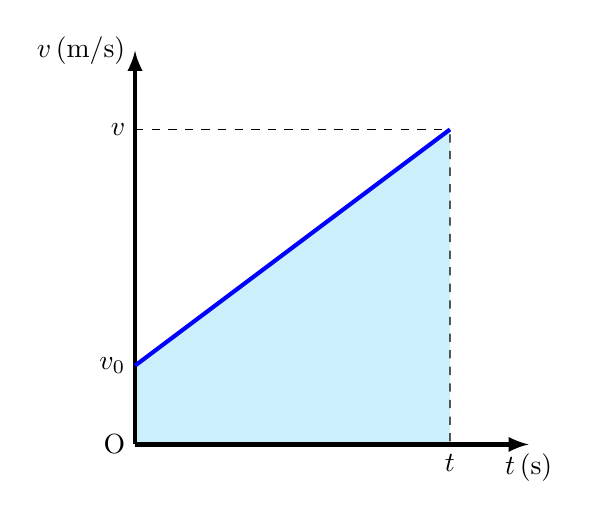
\begin{tikzpicture}  
					\coordinate (O) at(0,0);
					\coordinate (x) at(5,0);
					\coordinate (y) at(0,5);
					\coordinate (v0) at(0,1);
					\coordinate (v1) at(0,1.75);
					\coordinate (v2) at(0,4);
					\coordinate (B) at(4,4);
					\coordinate (A) at(1,1.75);
					\coordinate (C) at(4,0);
					\coordinate (D) at(1,0);
					\fill[cyan, opacity=0.2] (v0)--(B)--(C)--(O)--(v0);
					\draw[line width=0.5pt,black, dashed] (v0)--(B)--(C)--(O)--(v0);
					\draw[line width=0.5pt, dashed] (v2)--(B);
					\draw[-latex, line width=1.5pt] (O)--(x);
					\draw[-latex, line width=1.5pt] (O)--(y);
					\draw[blue, line width=1.5pt] (v0)--(B);
					\node[below] at(x) {$\xsi{t}{\left(\second\right)}$};
					\node[left] at(y) {$\xsi{v}{(\meter/\second)}$};
					\node[left] at(v0) {$v_0$};
					\node[left] at(0,4) {$v$};
					\node[left] at(O) {O};
					\node[below] at (C) {$t$};
				\end{tikzpicture}
			\end{center}
		}\\
		\multicolumn{2}{|L{17cm}|}{\dotfill}\\
		\multicolumn{2}{|L{17cm}|}{\dotfill}\\
		\multicolumn{2}{|L{17cm}|}{\dotfill}\\
		\multicolumn{2}{|L{17cm}|}{\dotfill}\\
		\hline
	\end{longtable}
\end{center}
\end{document}